\chapter{Black hole thermodynamics beyond general relativity}
\label{s:tha}

\minitoc

\section{Introduction}

This chapter is in a draft stage.

\medskip

This chapter relies heavily on exterior calculus, i.e. on calculus on differential forms.
The unfamiliar reader is urged to take a look at Sec.~\ref{s:bas:ext_deriv} of
Appendix~\ref{s:bas} first.

\section{Diffeomorphism-invariant theories of gravity}

\subsection{Framework} \label{s:tha:framework}

We consider that the $n$-dimensional spacetime $(\M,\w{g})$ is ruled by a metric theory of gravity built upon
a least action principle\index{least action}, with the following action:
\be \label{e:tha:action_L}
    \mathcal{S} = \int_{\M} \w{L} = \int_{\M} L \, \weps = \int_{\M} L \sqrt{-g} \, \D^n x .
\ee
Here $\w{L}$ is the \defin{Lagrangian $n$-form}\index{Lagrangian!form}\footnote{As the integral of a $n$-form over a $n$-dimensional manifold, $\mathcal{S}$ is well-posed and coordinate independent.},
$L$ is the \defin{Lagrangian scalar}\index{Lagrangian!scalar}
and
$\weps$ is the Levi-Civita tensor (cf. Sec.~\ref{s:bas:Levi-Civita_tensor}).
The second equality reflects the identity\footnote{Since the space of $n$-forms at any
point $p\in\M$ is 1-dimensional, $\w{L}$ and $\weps$ are
necessarily proportional, so that there is no loss of generality in the writing
$\w{L} = L \, \weps$.} $\w{L} = L \, \weps$ and the third one provides an expression of the integral
in terms of a coordinate system $(x^\alpha)$ on $\M$, $g$ being the determinant of
$\w{g}$ with respect to these coordinates [cf. Eq.~(\ref{e:bas:eps_sqrt_g})].
For simplicity we disregard any scalar or matter field, so that
$\w{L}$ is a function of the metric tensor $\w{g}$ only.
Actually all that follows can be easily generalized to account for
extra fields, as in scalar-tensor theories for instance, where $\w{L}$ is a function
of $\w{g}$ and some scalar field $\phi$. We limit ourselves here to $\w{g}$,
mostly in order to keep notations simple.
More precisely, we assume that at a given point $p\in\M$, $\w{L}$ depends only
on the values of $\w{g}$ and its derivatives at $p$, up to a certain order.
By \emph{derivative}, it is
meant derivative with respect to some affine connection on $\M$, for instance the one
formed by the partial derivatives with respect to given coordinates. We shall
write $\w{L}\lld\w{g}\rld$ to stress this dependency of $\w{L}$ on $\w{g}$, according
to the following convention:
\begin{notation}
\label{n:tha:bold_parentheses}
Boldface parentheses are used to denote the local (pointwise) dependency of a
tensor field on $\M$ with respect to other ones: $\w{A}\lld \w{B}, \w{C} \rld$
means that at a given point $p\in\M$, $\w{A}$ depends only
on the values of the tensor fields $\w{B}$ and $\w{C}$ and their derivatives at $p$.
\end{notation}

We shall consider only gravity theories whose
formulation does not depend upon any specific coordinates on $\M$, nor upon
any extra-structure on $\M$, like a privileged vector field.
This amounts to demanding that the
Lagrangian $n$-form $\w{L}$ is covariant under the group of diffeomorphisms of $\M$.
More precisely, under the action of a diffeomorphism $\Phi:\M \to \M$, the metric tensor
is transformed to its pullback $(\Phi^{-1})^*\w{g}$ by
$\Phi^{-1}$ (cf. Sec.~\ref{s:bas:push_pull} for the definition of the pullback).
The inverse of $\Phi$ is invoked here because, as $\w{g}$ is a
tensor of type $(0,2)$, $\Phi^*$ would carry it from\footnote{Since $\Phi$ is a diffeomorphism
$\M\to \M$, we have of course $\Phi(\M)=\M$; however we keep the notation $\Phi(\M)$ to stress the image character by $\Phi$.} $\Phi(\M)$ to $\M$, while
we are considering the transformation from $\M$ to $\Phi(\M)$ (cf. Remark~\ref{r:bas:comp_push_pull} on
p.~\pageref{r:bas:comp_push_pull}).
Let $\w{L}\lld(\Phi^{-1})^*\w{g}\rld$ be the Lagrangian $n$-form constructed by keeping the same functional
dependence in $(\Phi^{-1})^*\w{g}$ as $\w{L}\lld\w{g}\rld$ has in $\w{g}$.
The invariance of the theory under diffeomorphisms
amounts to demanding that, as a $n$-form on $\M$, $\w{L}\lld(\Phi^{-1})^*\w{g}\rld$ is nothing but
the $n$-form $\w{L}\lld\w{g}\rld$ transformed under the action of $\Phi$, i.e. the pullback of $\w{L}\lld\w{g}\rld$ by
$\Phi^{-1}$:  $\w{L}\lld(\Phi^{-1})^*\w{g}\rld = (\Phi^{-1})^*\w{L}\lld\w{g}\rld$.
Given that the spacetimes
$(\M, \w{g})$ and $(\Phi(\M),(\Phi^{-1})^* \w{g})$ are physically equivalent,
this means that $\w{L}\lld\w{g}\rld$ and $\w{L}\lld(\Phi^{-1})^*\w{g}\rld$ are basically the same object.
In particular, the action $\mathcal{S}$ given by Eq.~(\ref{e:tha:action_L}) takes the same value if
$\w{L}\lld(\Phi^{-1})^*\w{g}\rld$ is substituted for $\w{L}\lld\w{g}\rld$. If one interprets the diffeomorphism
action in a ``passive'' way, i.e. as a change of coordinates on $\M$, the
diffeomorphism-invariance condition simply means that the functional form of $L$
expressed in Eq.~(\ref{e:tha:Lagrangian_diffeo_inv}) below does not depend upon
the choice of coordinates. Since the condition  $\w{L}\lld(\Phi^{-1})^*\w{g}\rld = (\Phi^{-1})^*\w{L}\lld\w{g}\rld$
must hold for any diffeomorphism, we may simplify it
by introducing $\Phi' := \Phi^{-1}$ and
renaming $\Phi'$ to $\Phi$:
\begin{greybox}
A gravity theory is said
to be \defin{diffeomorphism-invariant}\index{diffeomorphism!invariance} iff
its Lagrangian $n$-form $\w{L}$ is \defin{covariant}\index{covariant} under the group
of diffeomorphisms of $\M$, i.e. iff for
any diffeomorphism $\Phi: \M \to \M$,
\be \label{e:tha:covariant_Lagrangian}
    \w{L}\lld\Phi^*\w{g}\rld = \Phi^*\w{L}\lld\w{g}\rld ,
\ee
where $\Phi^*$ stands for the pullback by $\Phi$, as defined in Sec.~\ref{s:bas:push_pull}.
\end{greybox}
We have then

\begin{prop}[Lagrangian of diffeomorphism-invariant theories
\textnormal{(Iyer\index[pers]{Iyer, V.} \& Wald\index[pers]{Wald, R.M.} 1994 \cite{IyerW94})}]
Any diffeomorphism-invariant theory of gravity based on a Lagrangian
involving only the metric tensor $\w{g}$ and a finite number of its derivatives (with respect to an arbitrary affine connection on $\M$) can be recast in terms of a Lagrangian involving only $\w{g}$, its
Riemann tensor and a finite number of symmetrized\footnote{There is no loss of generality in considering only symmetrized derivatives, since
any antisymmetrized combination can be reexpressed in term of the Riemann tensor itself and
lower order derivatives.} covariant derivatives of the latter:
\be \label{e:tha:Lagrangian_diffeo_inv}
    L\lld\w{g}\rld =
    L\left(g_{\alpha\beta}, R_{\alpha\beta\gamma\delta}, \nabla_\lambda R_{\alpha\beta\gamma\delta},\ldots,
    \nabla_{(\lambda_1} \cdots\nabla_{\lambda_m)} R_{\alpha\beta\gamma\delta} \right) .
\ee
\end{prop}
The reader is referred to the original article \cite{IyerW94} for the proof.

\begin{example}[Lagrangian of general relativity]
\label{x:tha:EH_Lagrangian}
For general relativity, $L$ is the Einstein-Hilbert Lagrangian\index{Einstein-Hilbert action}:
\be \label{e:tha:Hilbert_Lagrangian}
L = (16\pi)^{-1} R = (16\pi)^{-1} g^{\mu\nu} R_{\mu\nu}
 =  (16\pi)^{-1} g^{\mu\nu} R^\sigma_{\ \,\mu\sigma\nu}
 = (16\pi)^{-1} g^{\mu\nu} g^{\rho\sigma} R_{\rho\mu\sigma\nu} .
\ee
The last expression is clearly of the form (\ref{e:tha:Lagrangian_diffeo_inv}), given that
the components $(g^{\alpha\beta})$ are functions of the components $(g_{\alpha\beta})$ only.
\end{example}

\subsection{Lagrangian variation and presymplectic potential form}

A standard computation (see e.g \cite{Compe19,LeeW90}) leads to

\begin{prop}[variation of the Lagrangian of a pure metric theory]
\label{p:tha:var_Lagrangian}
Let $\w{L}$ be a Lagrangian $n$-form that depends only of the metric tensor $\w{g}$
and its derivatives, as in Eq.~(\ref{e:tha:Lagrangian_diffeo_inv}).
The variation of $\w{L}$ resulting from a generic variation $\delta\w{g}$ of $\w{g}$ is
expressible as
\be \label{e:tha:delta_L_E_Theta}
    \delta \w{L} = E^{\mu\nu} \delta g_{\mu\nu} \, \weps + \dd \w{\theta} ,
\ee
where $E^{\mu\nu}$ stands for the components of a symmetric type-$(2,0)$ tensor field $\w{E}$,
called the \defin{Euler-Lagrange tensor}\index{Euler-Lagrange!tensor},
and $\w{\theta}$ is a $(n-1)$-form, called the
\defin{presymplectic potential $(n-1)$-form}\index{presymplectic!potential form}
(this name will be justified below).
The $n$-form $\dd \w{\theta}$ is the exterior derivative of $\w{\theta}$
(cf. Sec.~\ref{s:bas:ext_deriv}).
$\w{E}$ depends on $\w{g}$ but \emph{not} on $\delta\w{g}$, while $\w{\theta}$
depends on both $\w{g}$ and $\delta\w{g}$, in a linear way in terms of $\delta\w{g}$.
All these dependencies are \emph{local}, so if we want to stress them, we shall write
$\w{E} = \w{E}\lld\w{g}\rld$ and $\w{\theta} = \w{\theta}\lld\w{g},\delta\w{g}\rld$
according to the notation introduced on p.~\pageref{n:tha:bold_parentheses}.
\end{prop}

\begin{remark}
The term $\dd\w{\theta}$ collects all the derivatives of $\delta\w{g}$, which have been gathered
by means of the Leibniz rule, so that the term $E^{\mu\nu} \delta g_{\mu\nu} \, \weps$
in Eq.~(\ref{e:tha:delta_L_E_Theta}) does not contain any derivative of $\delta\w{g}$.
\end{remark}

It must be stressed immediately that the presymplectic potential $(n-1)$-form
$\w{\theta}$ is not unique.
First of all, since
$\dd$ is nilpotent [Eq.~(\ref{e:ext_der_nilpot})], $\w{\theta}$ in formula~(\ref{e:tha:delta_L_E_Theta})
can be substituted by $\w{\theta'} = \w{\theta} + \dd \w{Y}$,
where $\w{Y}=\w{Y}\lld\w{g},\delta\w{g}\rld$ is an
arbitrary $(n-2)$-form. Secondly,
for a given gravity theory, the Lagrangian $n$-form itself is not unique.
Indeed the $n$-form
$\w{L'} = \w{L} + \dd\w{\mu}$, where $\w{\mu} = \w{\mu}\lld\w{g}\rld$ is an arbitrary $(n-1)$-form with compact
support, leads to the same action (\ref{e:tha:action_L}) by virtue of
Stokes' theorem (\ref{e:bas:Stokes}). The corresponding change in the presymplectic potential
is $\w{\theta} \to  \w{\theta} + \delta\w{\mu}$.
From these two facts, we conclude:

\begin{prop}[ambiguities in the presymplectic potential form]
\label{p:tha:ambiguities_theta}
For a given gravity theory, the presymplectic potential $(n-1)$-form $\w{\theta}$
is not unique: it can be substituted by
\be \label{e:tha:Theta_not_unique}
  \w{\theta'} = \w{\theta} + \dd \w{Y} + \delta\w{\mu},
\ee
where (i) $\w{Y}=\w{Y}\lld\w{g},\delta\w{g}\rld$ is an
arbitrary $(n-2)$-form that is a local function of $\w{g}$ and $\delta\w{g}$,
with a linear dependence on $\delta\w{g}$ and (ii)
$\delta\w{\mu}$ is the variation triggered by $\delta\w{g}$
of an arbitrary $(n-1)$-form $\w{\mu} = \w{\mu}\lld\w{g}\rld$
that is a local function of $\w{g}$ and has compact support.
The $\w{\mu}$ term in Eq.~(\ref{e:tha:Theta_not_unique}) arises from the allowed
change
\be \label{e:tha:L_not_unique}
    \w{L'} = \w{L} + \dd\w{\mu}
\ee
in the Lagrangian $n$-form.
\end{prop}


%\begin{remark} \label{r:tha:Lagrangian_dep_mu}
%For a given gravity theory, the Lagrangian $n$-form itself is not unique:
%\be \label{e:tha:Theta_gal_freedom}
%    \w{\theta'} = \w{\theta} + \dd \w{Y} + \delta\w{\mu},
%\ee

\begin{example}[presymplectic potential form of general relativity]
\label{x:tha:theta_GR}
For general relativity, one has $\w{L} = (16\pi)^{-1} R \weps$
[Eq.~(\ref{e:tha:Hilbert_Lagrangian})].
Given a coordinate system $(x^\alpha)$
on $\M$,
this can be rewritten as $\w{L} = (16\pi)^{-1} R \sqrt{-g} \, \w{e}$, where
$g$ is the determinant of $\w{g}$ with respect to $(x^\alpha)$ and
$\w{e}$ is the $n$-form whose components with respect to $(x^\alpha)$
are $e_{\alpha_1\cdots\alpha_n} = 1$ (resp. $-1$) if $(\alpha_1,\ldots,\alpha_n)$ is an
even (resp. odd) permutation of $(0,\ldots,n)$ and $0$ otherwise [cf. Eq.~(\ref{e:bas:eps_sqrt_g})].
One has then $\delta\w{L} = (16\pi)^{-1} \delta(R \sqrt{-g}) \, \w{e}$, since obviously $(x^\alpha)$, and thus
$\w{e}$, is not altered by the variation $\delta\w{g}$.
From the expression of $\delta(R\sqrt{-g})$ given by Eq.~(\ref{e:evo:proto_EH})
and using $G_{\mu\nu} \delta g^{\mu\nu} = - G^{\mu\nu} \delta g_{\mu\nu}$,
we get $16\pi\delta\w{L} = - G^{\mu\nu} \delta g_{\mu\nu} \, \weps + \nabla_\mu H^\mu \, \weps$,
where $G^{\mu\nu}$ is the double metric dual of the Einstein tensor and
$\w{H}$ is the vector field defined in terms of $\delta\w{g}$ by Eq.~(\ref{e:evo:def_H}),
where $h^\alpha_{\ \, \beta} = g^{\alpha\mu} \delta  g_{\mu\beta}$
since $h_{\alpha\beta}:= \delta g_{\alpha\beta}$. Now, the identity (\ref{e:bas:dveps_divv})
yields $\nabla_\mu H^\mu \,  \weps = \dd (\w{H}\cdot\weps)$, so that
$16\pi \delta\w{L} = - G^{\mu\nu} \delta g_{\mu\nu} \, \weps +  \dd (\w{H}\cdot\weps)$.
We conclude that the variation of the Einstein-Hilbert Lagrangian is indeed of the form
(\ref{e:tha:delta_L_E_Theta}) with
\be \label{e:tha:E_Theta_GR}
    E^{\alpha\beta} = - (16\pi)^{-1} \, G^{\alpha\beta}
    \qand
    \w{\theta} =  (16\pi)^{-1} \, \w{H}\cdot\weps = (16\pi)^{-1}\,  \star\!\uu{H} ,
\ee
where the last equality stems from the definition of the Hodge dual
of a 1-form [Eq.~(\ref{e:sta:Hodge_dual}) with $p=1$].
In index notation, $\theta_{\alpha_1\cdots\alpha_{n-1}} = (16\pi)^{-1}  H^\mu \eps_{\mu\alpha_1\cdots\alpha_{n-1}}$.
Substituting Eq.~(\ref{e:evo:def_H}) for $H^\mu$, we get the explicit expression of
$\w{\theta}\lld\w{g},\delta\w{g}\rld$:
\be \label{e:tha:Theta_GR}
    \theta_{\alpha_1\cdots\alpha_{n-1}} = (16\pi)^{-1}\, g^{\mu\nu} g^{\rho\sigma}
    \left( \nabla_\sigma \delta g_{\nu\rho} - \nabla_\nu \delta g_{\rho\sigma} \right)
    \epsilon_{\mu\alpha_1\cdots\alpha_{n-1}}  .
\ee
We check that $\w{\theta}\lld\w{g},\delta\w{g}\rld$ is linear in $\delta\w{g}$, as stated in Property~\ref{p:tha:var_Lagrangian}.
\end{example}

\begin{prop}[field equations from the least action principle]
The action $\mathcal{S}$ defined by (\ref{e:tha:action_L}) is extremal with respect to any
metric variation $\delta\w{g}$ that has compact support if, and only if,
\be \label{e:tha:eom_E}
    \w{E}\lld\w{g}\rld = 0 .
\ee
This constitutes the so-called \defin{Euler-Lagrange equations}\index{Euler-Lagrange!equation} for the considered gravity theory, also called the \defin{field equations}\index{field!equations} or
\defin{equations of motion}.
\end{prop}
\begin{proof}
Since $\delta\w{g}$ is assumed to have compact support, let $\mathscr{D}$ be
a $n$-dimensional submanifold with boundary of $\M$ such that
$\delta\w{g} = 0$ in the neighborhood of the boundary $\partial\mathscr{D}$ and outside $\mathscr{D}$.
In view of Eqs.~(\ref{e:tha:action_L}) and (\ref{e:tha:delta_L_E_Theta}), we have then
\[
    \delta \mathcal{S} = \int_\M \delta\w{L} = \int_{\mathscr{D}} E^{\mu\nu} \delta g_{\mu\nu} \, \weps
        + \int_{\mathscr{D}} \dd \w{\theta}
     = \int_{\mathscr{D}} E^{\mu\nu} \delta g_{\mu\nu} \, \weps
        + \underbrace{\int_{\partial\mathscr{D}} \w{\theta}}_{0}
     =  \int_{\mathscr{D}} E^{\mu\nu} \delta g_{\mu\nu} \, \weps ,
\]
where Stokes' theorem (\ref{e:bas:Stokes}) has been used to let appear the integral
of $\w{\theta}$ on $\partial\mathscr{D}$, which has been set to zero due
to $\left. \w{\theta}\lld\w{g},\delta\w{g}\rld \right|_{\partial\mathscr{D}} = 0$.
This last property results from the linearity of $\w{\theta}$ in $\delta\w{g}$, given that
$\delta\w{g}$ and all its derivatives are vanishing on $\partial\mathscr{D}$.
From the above expression of $\delta\mathcal{S}$ it is clear that having $\delta \mathcal{S} = 0$ for any variation $\delta\w{g}$ is equivalent to
Eq.~(\ref{e:tha:eom_E}).
\end{proof}

\begin{example}[field equations of general relativity]
\label{x:tha:field_equations_GR}
For general relativity, $\w{E}$ is given by Eq.~(\ref{e:tha:E_Theta_GR}).
Hence the field equations (\ref{e:tha:eom_E}) become $\w{G} = 0$, which
is equivalent to $\w{R}=0$ --- the
vacuum Einstein equation\index{Einstein!equation!vacuum --}\index{vacuum!Einstein equation}
(\ref{e:fra:vac_Einstein}).
\end{example}

\subsection{Noether charges related to diffeomorphism invariance}

Any smooth vector field $\w{\xi}$ on $\M$ generates a 1-parameter family of
infinitesimal diffeomorphisms, namely the flow maps along $\w{\xi}$:
$\Phi_t: \M \to \M$, where
$t$ is an infinitesimal parameter. As described in Sec.~\ref{s:bas:Lie_der_vector}, each $\Phi_t$ displaces any point $p\in\M$ by the infinitesimal vector $t\left.\w{\xi}\right| _p$.
The flow map $\Phi_t$ is clearly a diffeomorphism, whose inverse is $\Phi_t^{-1} = \Phi_{-t}$.
Let us consider the variation $\delta\w{g}$ induced by $\Phi_t$,
or more precisely by $\Phi_t^{-1}$ in order to simplify expressions;
indeed
choosing $\Phi_t^{-1}$ makes the pullback $\Phi_t^*\w{g}$ appear instead of
$(\Phi_t^{-1})^*\w{g}$, as discussed in Sec.~\ref{s:tha:framework}.
The variation of $\w{g}$ is then
\be \label{e:tha:delta_g_Phistar}
    \delta\w{g} = \Phi_t^* \w{g} - \w{g} .
\ee
Since $t$ is infinitesimal, the very definition of the
Lie derivative [Eq.~(\ref{e:bas:def_Lie_der_covar})] leads to
$\Phi_t^*\w{g} - \w{g} = t \Lie{\xi} \w{g}$.
It follows immediately that
\be  \label{e:bas:delta_g_Lie_xi_g}
    \delta\w{g} = t \Lie{\xi} \w{g} .
\ee
The variation of the Lagrangian $n$-form induced by $\delta\w{g}$
is $\delta\w{L} = \w{L}\lld\Phi_t^*\w{g}\rld - \w{L}\lld\w{g}\rld$.
Since the theory is assumed to be diffeomorphism-invariant, the covariance property
(\ref{e:tha:covariant_Lagrangian}) holds: $\w{L}\lld\Phi_t^*\w{g}\rld = \Phi_t^*\w{L}\lld\w{g}\rld$.
This yields $\delta\w{L} = \Phi_t^* \w{L}\lld\w{g}\rld - \w{L}\lld\w{g}\rld$. This
is the same form as $\w{g}$'s variation expressed in Eq.~(\ref{e:tha:delta_g_Phistar}) and, again, the
definition (\ref{e:bas:def_Lie_der_covar}) of the Lie derivative (which is applicable here since
$\w{L}$ is a tensor field of type $(0,n)$) leads to
\be \label{e:bas:delta_L_Lie_xi_L}
    \delta\w{L} = t \Lie{\xi} \w{L} .
\ee

\begin{remark}
The variation $\delta\w{g}$ is often defined as a \emph{variation rate} rather than a genuine variation, namely
as the \emph{derivative} of a 1-parameter family of metric tensors $\hat{\w{g}}(t)$ such that
$\hat{\w{g}}(0) = \w{g}$. Using the symbol $\hat\delta$ to distinguish from the variation considered here,
the definition is
$\hat{\delta}\w{g} := \left. \D{\hat{\w{g}}}/\D{t} \right|_{t=0}$.
Since the metric family induced by the flow maps along $\w{\xi}$ is
$\hat{\w{g}}(t) := \Phi_t^*\, \w{g}$, one gets
$\hat{\delta}\w{g} = \lim_{t\to 0} t^{-1} \left( \Phi_t^* \w{g} - \w{g} \right)$.
In view of the definition (\ref{e:bas:def_Lie_der_covar}) of the Lie derivative, this yields
\be \label{e:tha:hat_delta_g_Lie}
    \hat{\delta}\w{g} =  \Lie{\xi} \w{g} .
\ee
Similarly, one defines
$\hat{\delta}\w{L} :=  \left. \D{\w{L}\lld\hat{\w{g}}(t)\rld}/\D t \right|_{t=0}$,
which yields $\hat{\delta}\w{L} =  \Lie{\xi} \w{L}$.
When comparing with Eqs.~(\ref{e:bas:delta_g_Lie_xi_g}) and (\ref{e:bas:delta_L_Lie_xi_L}), we see that the derivative-based definition has the advantage of getting rid of the (not particularly significant) infinitesimal factor $t$.
\end{remark}

If one plugs Eqs.~(\ref{e:bas:delta_g_Lie_xi_g}) and (\ref{e:bas:delta_L_Lie_xi_L})
into the generic Lagrangian variation formula (\ref{e:tha:delta_L_E_Theta}), one gets
$t \Lie{\xi} \w{L}  = t E^{\mu\nu} \Liec{\xi} g_{\mu\nu} \,\weps + \dd( \w{\theta}\lld\w{g},t\Lie{\xi}\w{g}\rld)$.
Since $\w{\theta}$ is linear with respect to its second argument (cf. Property~\ref{p:tha:var_Lagrangian}),
one has
$\dd( \w{\theta}\lld\w{g},t\Lie{\xi}\w{g}\rld) =  t \dd( \w{\theta}\lld\w{g},\Lie{\xi}\w{g}\rld)$, so that there comes
\[
    \Lie{\xi} \w{L}  = E^{\mu\nu} \Liec{\xi} g_{\mu\nu} \,\weps + \dd( \w{\theta}\lld\w{g},\Lie{\xi}\w{g}\rld) .
\]
Now, the Cartan identity (\ref{e:bas:Cartan}) gives
$\Lie{\xi} \w{L} = \w{\xi} \cdot\dd \w{L} + \dd(\w{\xi}\cdot\w{L}) = \dd(\w{\xi}\cdot\w{L})$
since $\dd \w{L} = 0$, as for any $(n+1)$-form on a $n$-dimensional manifold.
Accordingly, we may rewrite the above equation as
\be \label{e:tha:dd_pre_J_E}
    \dd\left(  \w{\theta}\lld\w{g},\Lie{\xi}\w{g}\rld - \w{\xi}\cdot\w{L} \right) =
    - E^{\mu\nu} \Liec{\xi} g_{\mu\nu} \,\weps .
\ee
If the field equations are fulfilled, i.e. if $\w{E} = 0$ [Eq.~(\ref{e:tha:eom_E})], the
right-hand side of Eq.~(\ref{e:tha:dd_pre_J_E}) is zero, which implies that the
argument of the exterior derivative in the left-hand side is a closed
$(n-1)$-form. This defines a conserved current, which is nothing but the expression
of Noether's theorem\index{Noether's theorem} for the invariance of the Lagrangian by the 1-dimensional
group of diffeomorphisms generated by the vector field $\w{\xi}$:

\begin{prop}[Noether theorem for diffeomorphisms generated by a vector field]
\label{p:tha:Noether_current}
Given a smooth vector field $\w{\xi}$ on $\M$,
the \defin{Noether current $(n-1)$-form of $\w{\xi}$}\index{Noether!current form} is defined by \cite{Wald93,IyerW94}
\be \label{e:tha:def_Noether_current}
    \w{J}\lld\w{\xi}\rld := \w{\theta}\lld\w{g},\Lie{\xi}\w{g}\rld - \w{\xi}\cdot\w{L} ,
\ee
where $\w{\theta}\lld\w{g},\Lie{\xi}\w{g}\rld$ is the $(n-1)$-form obtained
by substituting $\Lie{\xi}\w{g}$ for $\delta\w{g}$ in the
presymplectic potential form $\w{\theta}\lld\w{g},\delta\w{g}\rld$
(cf. Property~\ref{p:tha:var_Lagrangian}) and $\w{\xi}\cdot\w{L}$
is the $(n-1)$-form obtained by setting the first argument of the $n$-form $\w{L}$
to $\w{\xi}$:  $\w{\xi}\cdot\w{L} := \w{L}(\w{\xi},\cdots)$.
$\w{J}\lld\w{\xi}\rld$ is a local function of $\w{\xi}$ and its derivatives,
and depends linearly on $\w{\xi}$.
If the gravity theory is diffeomorphism-invariant, then
the $(n-1)$-form $\w{J}\lld\w{\xi}\rld$ is closed as soon as the equations of motion (\ref{e:tha:eom_E}) are fulfilled  or $\w{\xi}$ is a Killing vector:
\be \label{e:tha:J_closed}
    \encadre{ \dd \w{J}\lld\w{\xi}\rld  = 0 }.
\ee
The Noether current $(n-1)$-form is not unique,
some ambiguity $\w{J} \to \w{J'}$ resulting from (\ref{e:tha:Theta_not_unique})
and (\ref{e:tha:L_not_unique}), with
\be \label{e:tha:J_not_unique}
     \w{J'}\lld\w{\xi}\rld =  \w{J}\lld\w{\xi}\rld  + \dd \left[ \w{Y}\lld\w{g},\Lie{\xi}\w{g}\rld
     + \w{\xi}\cdot\w{\mu}\lld\w{g}\rld\right],
\ee
where $\w{Y}\lld\w{g},\Lie{\xi}\w{g}\rld$ is any $(n-2)$-form that is linear in $\Lie{\xi}\w{g}$,
$\w{\mu}\lld\w{g}\rld$ is any $(n-1)$-form with compact support and $\w{\xi}\cdot\w{\mu}$
is the $(n-2)$-form $\w{\mu}(\w{\xi},\ldots)$.
\end{prop}

\begin{proof}
That $\w{J}\lld\w{\xi}\rld$ is a linear function of $\w{\xi}$ follows immediately from
the linearity of $\w{\theta}\lld .,.\rld$ with respect to its second argument. Similarly the
locality of $\w{J}\lld\w{\xi}\rld$ with respect of $\w{\xi}$ is inherited from
that of $\w{\theta}\lld .,.\rld$.
If the theory diffeomorphism-invariant, Eq.~(\ref{e:tha:dd_pre_J_E}) holds. Given the
definition of $\w{J}\lld\w{\xi}\rld$, Eq.~(\ref{e:tha:dd_pre_J_E}) is equivalent to
$\dd\w{J}\lld\w{\xi}\rld  = - E^{\mu\nu} \Liec{\xi} g_{\mu\nu} \,\weps$,
so that $\dd\w{J}\lld\w{\xi}\rld  = 0$ if $\w{E} = 0$ is fulfilled or $\w{\xi}$ is a Killing vector ($\Lie{\xi}\w{g} = 0$). Finally,
both $\w{L'}\lld\w{g}\rld$ and $\w{L}\lld\w{g}\rld$
in Eq.~(\ref{e:tha:L_not_unique})
must be covariant under diffeomorphisms. It follows that
$\w{\mu}\lld\w{g}\rld$ must be covariant as well. Then the variation of $\w{\mu}$
resulting from a diffeomorphism $\Phi_t$ generated by $\w{\xi}$ is
$\delta\w{\mu} = t \Lie{\xi}\w{\mu}$, by the very same argument that led to
formula~(\ref{e:bas:delta_L_Lie_xi_L}) for $\delta\w{L}$. Accordingly,
Eq.~(\ref{e:tha:Theta_not_unique}) yields
$\w{\theta'}\lld\w{g},\Lie{\xi}\w{g}\rld = \w{\theta}\lld\w{g},\Lie{\xi}\w{g}\rld +
\dd \w{Y}\lld\w{g},\Lie{\xi}\w{g}\rld +  \Lie{\xi}\w{\mu}\lld\w{g}\rld$.
By combining this identity with $\w{L'} = \w{L} + \dd\w{\mu}$ [Eq.~(\ref{e:tha:L_not_unique})],
the definition~(\ref{e:tha:def_Noether_current}) applied to $\w{J'}$ leads to
\[
    \w{J'}\lld\w{\xi}\rld =  \w{J}\lld\w{\xi}\rld  + \dd \w{Y}\lld\w{g},\Lie{\xi}\w{g}\rld
     + \Lie{\xi}\w{\mu}\lld\w{g}\rld
     - \w{\xi}\cdot\dd\w{\mu}\lld\w{g}\rld .
\]
The Cartan identity (\ref{e:bas:Cartan}) gives
$\Lie{\xi}\w{\mu}\lld\w{g}\rld - \w{\xi}\cdot\dd\w{\mu}\lld\w{g}\rld  = \dd\left( \w{\xi}\cdot\w{\mu}\lld\w{g}\rld \right)$
and we obtain (\ref{e:tha:J_not_unique}).
\end{proof}

\begin{remark}
\label{r:tha:notation_J}
From the definition (\ref{e:tha:def_Noether_current}), it is clear that
$\w{J}\lld\w{\xi}\rld$ is a local function of $\w{g}$ (and its derivatives), in addition to $\w{\xi}$. So, following the notation introduced in Sec.~\ref{s:tha:framework}, we could have written
$\w{J}\lld\w{g},\w{\xi}\rld$. However for the sake of brevety, we use
$\w{J}\lld\w{\xi}\rld$, leaving the dependency on $\w{g}$ implicit.
\end{remark}

\begin{example}[Noether current form of general relativity]
From expression (\ref{e:tha:Theta_GR}) for $\w{\theta}$ in general relativity
with $\delta g_{\mu\nu} = t \Liec{\xi} g_{\mu\nu} = t(\nabla_\mu \xi_\nu + \nabla_\nu \xi_\mu)$[Eq.~(\ref{e:bas:Lie_g_Killing})], we get
\bea
 16\pi   \theta\lld\w{g},\Lie{\xi}\w{g}\rld_{\alpha_1\cdots\alpha_{n-1}} & = &
  g^{\mu\nu} \left( \nabla_\sigma \nabla_\nu \xi^\sigma + \nabla_\sigma \nabla^\sigma \xi_\nu
    - 2 \nabla_\nu \nabla_\rho \xi^\rho \right) \epsilon_{\mu\alpha_1\cdots\alpha_{n-1}} \nonumber \\
    & = & g^{\mu\nu} \left( 2 R_{\nu\sigma} \xi^\sigma - \nabla_\sigma \nabla_\nu \xi^\sigma
     + \nabla_\sigma \nabla^\sigma \xi_\nu \right) \epsilon_{\mu\alpha_1\cdots\alpha_{n-1}} \nonumber \\
    & = & \left( 2 R^\mu_{\ \, \nu} \xi^\nu + \nabla_\nu \nabla^\nu \xi^\mu - \nabla_\nu \nabla^\mu \xi^\nu
        \right) \epsilon_{\mu\alpha_1\cdots\alpha_{n-1}} , \nonumber
\eea
where the contracted Ricci identity (\ref{e:bas:contract_Ricci_ident}) has been used to get the second
line. Plugging this formula, as well as $\w{L} = R \weps$ (cf. Example~\ref{x:tha:EH_Lagrangian}) into
the definition (\ref{e:tha:def_Noether_current}) of $\w{J}\lld\w{\xi}\rld$ yields
\[
    J\lld\w{\xi}\rld_{\alpha_1\cdots\alpha_{n-1}} = (16\pi)^{-1} \left(2 G^\mu_{\ \, \nu} \xi^\nu +
        \nabla_\nu \nabla^\nu \xi^\mu - \nabla_\nu \nabla^\mu \xi^\nu \right) \epsilon_{\mu\alpha_1\cdots\alpha_{n-1}} .
\]
If the field equations are obeyed, then $\w{G}=0$ (cf. Example~\ref{x:tha:field_equations_GR}) and the above
expression reduces to
\be \label{e:tha:J_GR_comp}
    J\lld\w{\xi}\rld_{\alpha_1\cdots\alpha_{n-1}} = (16\pi)^{-1} \left(
        \nabla_\nu \nabla^\nu \xi^\mu - \nabla_\nu \nabla^\mu \xi^\nu \right) \epsilon_{\mu\alpha_1\cdots\alpha_{n-1}} .
\ee
We recognize in the term within parentheses the \emph{Komar current of $\w{\xi}$}\index{Komar!current}\index{current!Komar --}  as defined by Eq.~(\ref{e:sta:def_Komar_current}):
$\mathcal{J}\lld\w{\xi}\rld^\mu := \nabla_\nu \nabla^\nu \xi^\mu - \nabla_\nu \nabla^\mu \xi^\nu$.
Accordingly, we may write
\be \label{e:tha:J_GR_Komar}
    \w{J}\lld\w{\xi}\rld = (16\pi)^{-1}\, \w{\mathcal{J}}\lld\w{\xi}\rld  \cdot \weps
    = (16\pi)^{-1} \star\uu{\mathcal{J}}\lld\w{\xi}\rld  ,
\ee
where the last equality stems from Eq.~(\ref{e:sta:Hodge_dual}) with $p=1$.
Hence, for general relativity, the Noether current $(n-1)$-form of $\w{\xi}$ is nothing but the
Hodge dual of the (metric dual of the) Komar current of $\w{\xi}$, up to the factor
$(16\pi)^{-1}$.
That $\w{J}\lld\w{\xi}\rld$ is closed in this case follows readily from the identity (\ref{e:bas:dveps_divv}):
$16\pi \, \dd\w{J}\lld\w{\xi}\rld = \dd( \w{\mathcal{J}}\lld\w{\xi}\rld \cdot \weps ) = (\wnab\cdot\w{\mathcal{J}}\lld\w{\xi}\rld) \weps$, along
with the conservation law (\ref{e:sta:divJ_zero}): $\wnab\cdot\w{\mathcal{J}}\lld\w{\xi}\rld = 0$.
\end{example}

\begin{prop}[Noether potential form]
\label{p:tha:Noether_pot_form}
Given a vector field $\w{\xi}$ on $\M$ and a diffeomorphism-invariant theory described by a Lagrangian $n$-form $\w{L}$, there exists a $(n-2)$-form $\w{Q}\lld\w{\xi}\rld$ on $\M$,
which is a linear local function of $\w{\xi}$, such that
the Noether current $(n-1)$-form of $\w{\xi}$ is the exterior derivative of $\w{Q}\lld\w{\xi}\rld$:
\be \label{e:tha:J_dQ}
    \w{J}\lld\w{\xi}\rld = \dd \w{Q}\lld\w{\xi}\rld .
\ee
$\w{Q}\lld\w{\xi}\rld$ is called the \defin{Noether potential $(n-2)$-form of $\w{\xi}$}\index{Noether!potential!form}. It is not unique, being subject to the ambiguity
$\w{Q} \to \w{Q'}$, with
\be \label{e:tha:Q_not_unique}
    \w{Q'}\lld\w{\xi}\rld = \w{Q}\lld\w{\xi}\rld + \w{Y}\lld\w{g},\Lie{\xi}\w{g}\rld
     + \w{\xi}\cdot\w{\mu}\lld\w{g}\rld + \dd\w{Z}\lld\w{g},\w{\xi}\rld ,
\ee
where $\w{Y}\lld\w{g},\Lie{\xi}\w{g}\rld$ is any $(n-2)$-form that is linear in $\Lie{\xi}\w{g}$, $\w{\mu}\lld\w{g}\rld$ is any $(n-1)$-form with compact support
and
$\w{Z}\lld\w{g},\w{\xi}\rld $ is any $(n-3)$-form that is linear in $\w{\xi}$.
\end{prop}

\begin{proof}
Since $\w{J}\lld\w{\xi}\rld$ is a closed differential form [Eq.~(\ref{e:tha:J_closed})], the Poincaré lemma
states that it is \emph{locally} exact (on a contractible open set, cf. Sec.~\ref{s:bas:ext_deriv}). However, because
$\dd \w{J}\lld\w{\xi}\rld  = 0$ holds for any vector field $\w{\xi}$, it can be shown that
$\w{J}\lld\w{\xi}\rld$ is \emph{globally} exact, i.e. takes the form (\ref{e:tha:J_dQ})
with $\w{Q}\lld\w{\xi}\rld$ being a local function of $\w{\xi}$ \cite{Wald90}.
The linearity of $\w{Q}\lld\w{\xi}\rld$ in terms of $\w{\xi}$ arises from the linearity
of $\w{J}\lld\w{\xi}\rld$ (cf. Property~\ref{p:tha:Noether_current}).
Finally, the $\w{Y}$ and $\w{\mu}$ ambiguities in (\ref{e:tha:Q_not_unique}) are inherited from the ambiguities of $\w{J}$ [Eq.~(\ref{e:tha:J_not_unique})], while the $\w{Z}$ ambiguity stems from Eq.~(\ref{e:tha:J_dQ}) defining
$\w{Q}$ up to the addition of a closed $(n-2)$-form (cf. Lemma~1 in Ref.~\cite{Wald90}).
\end{proof}

\begin{remark}
\label{r:tha:notation_Q}
As for $\w{J}\lld\w{\xi}\rld$ (cf. Remark~\ref{r:tha:notation_J} on p.~\pageref{r:tha:notation_J}), $\w{Q}\lld\w{\xi}\rld$ is a local function of $\w{g}$, in addition
to $\w{\xi}$, although the dependency on $\w{g}$ is not explicited in the notation
$\w{Q}\lld\w{\xi}\rld$.
\end{remark}

\begin{remark}
The $(n-2)$-form $\w{Q}\lld\w{\xi}\rld$ has been introduced by Wald (1993) \cite{Wald93} under
the name \emph{Noether charge $(n-2)$-form}. However, as argued by
other authors \cite{JacobKM94,HarloW20}, the name
\emph{Noether potential $(n-2)$-form} is more relevant, since $\w{Q}\lld\w{\xi}\rld$
is not conserved: a priori $\dd\w{Q}\lld\w{\xi}\rld \neq 0$ and Eq.~(\ref{e:tha:J_dQ}) shows
clearly that $\w{Q}\lld\w{\xi}\rld$ plays the role of a potential of a conserved current.
Another name given to $\w{Q}\lld\w{\xi}\rld$ in the literature is
the \emph{Noether-Wald charge density}\index{Noether-Wald charge density}
\cite{GrumiS22,HajiaS16}.
\end{remark}

\begin{example}[Noether potential form of general relativity]
\label{x:tha:Noether_potential_form_GR}
For general relativity, $\w{J}\lld\w{\xi}\rld$ is given by Eq.~(\ref{e:tha:J_GR_comp}), or Eq.~(\ref{e:tha:J_GR_Komar}) in terms of the Komar current of $\w{\xi}$.
Let us show that $\w{Q}\lld\w{\xi}\rld$ is then nothing but the Hodge dual of the exterior derivative
of the 1-form $\uu{\xi}$ (the metric dual to $\w{\xi}$), up to the factor $-(16\pi)^{-1}$:
\be \label{e:tha:Q_GR_Komar}
    \w{Q}\lld\w{\xi}\rld = - (16\pi)^{-1}\, \star (\dd \uu{\xi}) .
\ee
Given the expression of the Hodge dual
of a 2-form [Eq.~(\ref{e:sta:Hodge_dual}) with $p=2$], the identity
$(\dd\uu{\xi})_{\alpha\beta} = \nabla_\alpha  \xi_\beta - \nabla_\beta \xi_\alpha$
[Eq.~(\ref{e:bas:def_ext_1f_nab})] and the antisymmetry of $\weps$, a formula
equivalent to (\ref{e:tha:Q_GR_Komar}) is
\be \label{e:tha:Noether_Q_GR}
    Q\lld\w{\xi}\rld_{\alpha_1\cdots\alpha_{n-2}} = -  (16\pi)^{-1}\,  \nabla^\mu \xi^\nu
        \eps_{\mu\nu\alpha_1\cdots\alpha_{n-2}} .
\ee
To prove that $\w{Q}\lld\w{\xi}\rld$ as given by (\ref{e:tha:Q_GR_Komar}) obeys
$\dd\w{Q}\lld\w{\xi}\rld = \w{J}\lld\w{\xi}\rld$ [Eq.~(\ref{e:tha:J_dQ})], let us establish the
Hodge dual of this relation: $\star\dd\w{Q}\lld\w{\xi}\rld = \star\w{J}\lld\w{\xi}\rld$,
which is an equality between 1-forms. From Eq.~(\ref{e:tha:Q_GR_Komar}), we have
$\star\dd\w{Q}\lld\w{\xi}\rld = - (16\pi)^{-1}\,  \star\dd \star (\dd \uu{\xi})$.
Now, the operator $\star\dd\star$ is, up to a sign, the \defin{codifferential}\index{codifferential}
$\w{\delta}$, which maps a $p$-form to a $(p-1)$-form and is defined by\footnote{See e.g. Eq.~(14.35) of Straumann's book \cite{Strau13}, whose sign
convention is followed here. Since the same letter $\delta$
is used to denote the codifferential and the variation operator,
we are using a boldface symbol to distinguish the former.}
$\w{\delta} := (-1)^{n(p+1)+1} \star\dd\star$. Since $\dd \uu{\xi}$ is a 2-form, we get
$\star\dd\w{Q}\lld\w{\xi}\rld = (-1)^n (16\pi)^{-1}\, \w{\delta}(\dd \uu{\xi})$. From the expression of the
codifferential in a coordinate chart $(x^\alpha)$ (cf. e.g. Eq.~(14.37) in Ref.~\cite{Strau13}), we may
write, for any 2-form $\w{A}$:
\[
        (\w{\delta}\w{A})^\alpha = \frac{1}{\sqrt{-g}} \der{}{x^\mu} \left(\sqrt{-g} A^{\mu\alpha} \right)
            = - \nabla_\mu A^{\alpha\mu} ,
\]
where the last equality follows from the identity (\ref{e:bas:div_antisym}).
Applying the above formula to $\w{A} := \dd\uu{\xi}$,  we get
$\w{\delta}(\dd\uu{\xi})^\alpha = - \nabla_\mu (\nabla^\alpha \xi^\mu - \nabla^\mu \xi^\alpha) = \mathcal{J}\lld\w{\xi}\rld^\alpha$, i.e. $\w{\delta}(\dd\uu{\xi}) = \uu{\mathcal{J}}\lld\w{\xi}\rld$,
where $\w{\mathcal{J}}\lld\w{\xi}\rld$ is the Komar current of $\w{\xi}$
defined by Eq.~(\ref{e:sta:def_Komar_current}).
Hence $\star\dd\w{Q}\lld\w{\xi}\rld = (-1)^n (16\pi)^{-1}\, \uu{\mathcal{J}}\lld\w{\xi}\rld$. On the other hand, we have
$\star \w{J}\lld\w{\xi}\rld =(16\pi)^{-1}\, \star \star\uu{\mathcal{J}}\lld\w{\xi}\rld$ from
Eq.~(\ref{e:tha:J_GR_Komar}). Since $\star\star = (-1)^n \mathrm{Id}$ for a 1-form
(cf. e.g. formula (14.26) in Ref.~\cite{Strau13}), we immediately get
$\star \w{J}\lld\w{\xi}\rld  = \star\dd\w{Q}\lld\w{\xi}\rld$, which is equivalent to
Eq.~(\ref{e:tha:J_dQ}).
\end{example}


\begin{prop}[Noether charge of a spacelike hypersurface]
\label{p:tha:Noether_charge_hypersurf}
Let us consider a diffeomorphism-invariant theory described by a Lagrangian $n$-form $\w{L}$.
Given a vector field $\w{\xi}$ on $\M$ and
a spacelike hypersurface $\Sigma$, the
\defin{Noether charge of $\Sigma$ with respect to $\w{\xi}$}\index{Noether!charge!of a hypersurface} is
\be \label{e:tha:def_Q_hypersurf}
    \mathscr{Q}_{\Sigma,\w{\xi}} := \int_{\Sigma} \w{J}\lld\w{\xi}\rld ,
\ee
where $\w{J}\lld\w{\xi}\rld$ is the Noether current $(n-1)$-form of $\w{\xi}$ (Property~\ref{p:tha:Noether_current})
and the integral is taken with respect to $\Sigma$ endowed with the \defin{future orientation},
i.e. the orientation defined by $\w{n}\cdot\weps$, where $\w{n}$ is the future-directed timelike unit normal
to $\Sigma$. The Noether charge is a priori not unique, since any change $\w{J} \to \w{J'}$
allowed by (\ref{e:tha:J_not_unique}) leads to $\mathscr{Q}_{\Sigma,\w{\xi}} \to \mathscr{Q'}_{\Sigma,\w{\xi}}$
with
\be \label{e:tha:Q_hyper_not_unique}
    \mathscr{Q'}_{\Sigma,\w{\xi}} = \mathscr{Q}_{\Sigma,\w{\xi}} +
    \int_{\partial\Sigma} \left[ \w{Y}\lld\w{g},\Lie{\xi}\w{g}\rld
     + \w{\xi}\cdot\w{\mu}\lld\w{g}\rld \right] .
\ee
However, if $\w{\xi}$ is a Killing vector and (i) $\w{\xi}$ is tangent to $\partial\Sigma$
or (ii) $\partial\Sigma$ is located outside the support of $\w{\mu}\lld\w{g}\rld$,
the Noether charge is
uniquely defined: $\mathscr{Q'}_{\Sigma,\w{\xi}} = \mathscr{Q}_{\Sigma,\w{\xi}}$.

Let $\Sigma_1$ and $\Sigma_2$ be two spacelike hypersurfaces, such that $\Sigma_2$ lies
in the future of $\Sigma_1$ and both hypersurfaces are connected by a hypersurface $\mathscr{W}$, i.e.
$\Sigma_1\cup\Sigma_2\cup\mathscr{W}$ is a closed hypersurface consituting
the boundary of a $n$-dimensional manifold  $\mathscr{D}\subset\M$ (cf. Fig.~??).
Then the following conservation law holds:
\be \label{e:tha:Noether_Q_Sigma_1_2}
    \encadre{ \mathscr{Q}_{\Sigma_2,\w{\xi}}  = \mathscr{Q}_{\Sigma_1,\w{\xi}}
    + \int_{\mathscr{W}^{\swarrow}} \w{J}\lld\w{\xi}\rld },
\ee
where the integral over $\mathscr{W}$ is taken with respect to the \emph{inward} orientation (indicated by
the arrow), i.e. the orientation
defined by $\w{v}\cdot\weps$, where $\w{v}$ is any vector field pointing into $\mathscr{D}$.
\end{prop}

\begin{proof}
Equation~(\ref{e:tha:Q_hyper_not_unique}) readily follows from (\ref{e:tha:J_not_unique}) and
Stokes' theorem (\ref{e:bas:Stokes}). If $\w{\xi}$ is a Killing vector, then
$\Lie{\xi}\w{g}= 0$ by definition (cf. Property~\ref{p:def_Killing_vector}); this implies
$\w{Y}\lld\w{g},\Lie{\xi}\w{g}\rld = 0$ in the
right-hand side of Eq.~(\ref{e:tha:Q_hyper_not_unique}), given that
$\w{Y}$ is linear with respect to $\Lie{\xi}\w{g}$.
Moreover, if $\w{\xi}$ is tangent to $\partial\Sigma$ (case (i)), the $(n-2)$-form
$\w{\xi}\cdot\w{\mu} = \w{\mu}(\w{\xi},\ldots)$ restricted to vectors tangent to $\partial\Sigma$
is necessarily zero, for $\w{\mu}$ is a $(n-1)$-form. Obviously, this holds as well in the case (ii).
Hence
$\mathscr{Q'}_{\Sigma,\w{\xi}} = \mathscr{Q}_{\Sigma,\w{\xi}}$.
As for Eq.~(\ref{e:tha:Noether_Q_Sigma_1_2}),
given that $\partial\mathscr{D} = \Sigma_1\cup\Sigma_2\cup\mathscr{W}$, Stokes' theorem (\ref{e:bas:Stokes})
and $\dd \w{J}\lld\w{\xi}\rld = 0$ [Eq.~(\ref{e:tha:J_closed})] lead to
\[
     \int_{\Sigma_1^{\nearrow}} \w{J}\lld\w{\xi}\rld + \int_{\Sigma_2^{\nearrow}} \w{J}\lld\w{\xi}\rld
      + \int_{\mathscr{W}^{\nearrow}} \w{J}\lld\w{\xi}\rld = 0 ,
\]
where the arrows mean that $\Sigma_1$, $\Sigma_2$ and $\mathscr{W}$ are oriented according to the outward
convention (with respect to $\mathscr{D}$).
Noticing that $\int_{\Sigma_1^{\nearrow}} \w{J}\lld\w{\xi}\rld = -\mathscr{Q}_{\Sigma_1,\w{\xi}}$,
$\int_{\Sigma_2^{\nearrow}} \w{J}\lld\w{\xi}\rld = \mathscr{Q}_{\Sigma_2,\w{\xi}}$
and $\int_{\mathscr{W}^{\nearrow}} \w{J}\lld\w{\xi}\rld = - \int_{\mathscr{W}^{\swarrow}} \w{J}\lld\w{\xi}\rld$
yields (\ref{e:tha:Noether_Q_Sigma_1_2}).
\end{proof}

The integral over $\mathscr{W}$ in Eq.~(\ref{e:tha:Noether_Q_Sigma_1_2}) can be interpreted as
an ``inward flux'', especially if $\mathscr{W}$ is a timelike hypersurface
(cf. the electromagnetic analogy detailed in Remark~\ref{r:tha:charge_em_analogy} below).
If this inward flux vanishes,
Eq.~(\ref{e:tha:Noether_Q_Sigma_1_2}) expresses the
invariance of the Noether charge with respect to the choice of the hypersurface
(conservation during ``time evolution''). This occurs
if $\w{J}\lld\w{\xi}\rld = 0$ on $\mathscr{W}$ or if  $\mathscr{W}$ is at some asymptotically flat end
of $\M$ with $\w{J}\lld\w{\xi}\rld$ decaying sufficiently fast so that its integral on $\mathscr{W}$ is zero.

\begin{prop}[Noether charge of a closed spacelike $(n-2)$-surface]
\label{p:tha:Noether_charge_surf}
Let us consider a diffeomorphism-invariant theory described by a Lagrangian $n$-form $\w{L}$
and let assume that $(\M,\w{g})$ is asymptotically flat.
Given a vector field $\w{\xi}$ on $\M$
and a closed spacelike $(n-2)$-surface $\Sp\subset\M$, the
\defin{Noether charge of $\Sp$ with respect to $\w{\xi}$}\index{Noether!charge!of a surface} is
\be \label{e:tha:def_Noether_Q_surf}
    \mathscr{Q}_{\Sp,\w{\xi}} := \int_{\Sp} \w{Q}\lld\w{\xi}\rld ,
\ee
where $\w{Q}\lld\w{\xi}\rld$ is the Noether potential $(n-2)$-form of $\w{\xi}$
(Property~\ref{p:tha:Noether_pot_form}) and the orientation of $\Sp$ for the above integral is the \emph{future-outward} orientation
defined by Eq.~(\ref{e:sta:def_weps_S}).
The Noether charge is a priori not unique, since any change $\w{Q} \to \w{Q'}$
obeying (\ref{e:tha:Q_not_unique}) leads to $\mathscr{Q}_{\Sp,\w{\xi}} \to \mathscr{Q'}_{\Sp,\w{\xi}}$
with
\be \label{e:tha:Q_surf_not_unique}
    \mathscr{Q'}_{\Sp,\w{\xi}} = \mathscr{Q}_{\Sp,\w{\xi}}
    + \int_{\Sp} \left[ \w{Y}\lld\w{g},\Lie{\xi}\w{g}\rld
     + \w{\xi}\cdot\w{\mu}\lld\w{g}\rld \right] .
\ee
However, if $\w{\xi}$ is a Killing vector and (i) $\w{\xi}$ is tangent to $\Sp$
or (ii) $\Sp$ is located outside the support of $\w{\mu}\lld\w{g}\rld$,
the Noether charge is
uniquely defined: $\mathscr{Q'}_{\Sp,\w{\xi}} = \mathscr{Q}_{\Sp,\w{\xi}}$.

Let $\Sigma$ be a compact spacelike hypersurface bounded by two closed $(n-2)$-surfaces:
an ``internal'' one, $\Sp_{\rm int}$, and an ``external'' one,
$\Sp_{\rm ext}$, the exterior direction being that of the asymptotic flat end of $(\M, \w{g})$.
Then
\be \label{e:tha:Noether_Q_S_ext_int}
     \encadre{ \mathscr{Q}_{\Sp_{\rm ext},\w{\xi}} = \mathscr{Q}_{\Sp_{\rm int},\w{\xi}}
        + \mathscr{Q}_{\Sigma,\w{\xi}}  }.
\ee
\end{prop}

\begin{proof}
Equation~(\ref{e:tha:Q_surf_not_unique}) readily follows from (\ref{e:tha:Q_not_unique})
along with $\int_{\Sp} \dd\w{Z} = 0$ as a result of Stokes' theorem (\ref{e:bas:Stokes}),
given that $\Sp$ is a closed manifold:
$\partial\Sp = \varnothing$.
The proof that $\mathscr{Q'}_{\Sp,\w{\xi}} = \mathscr{Q}_{\Sp,\w{\xi}}$
in the considered cases is identical to the proof of $\mathscr{Q'}_{\Sigma,\w{\xi}} = \mathscr{Q}_{\Sigma,\w{\xi}}$
in Property~\ref{p:tha:Noether_charge_hypersurf}.
Finally, to prove (\ref{e:tha:Noether_Q_S_ext_int}),
let us substitute $\dd\w{Q}$ for $\w{J}$ [cf. Eq.~(\ref{e:tha:J_dQ})]
in expression (\ref{e:tha:def_Q_hypersurf}) of
$\mathscr{Q}_{\Sigma,\w{\xi}}$. Applying
Stokes' theorem (\ref{e:bas:Stokes}) and using
$\partial\Sigma = \Sp_{\rm int} \cup \Sp_{\rm ext}$, we get
\[
    \mathscr{Q}_{\Sigma,\w{\xi}} = \int_{\Sp_{\rm int}^\nearrow} \w{Q}\lld\w{\xi}\rld
    + \int_{\Sp_{\rm ext}^\nearrow} \w{Q}\lld\w{\xi}\rld ,
\]
where the arrows indicate that $\Sp_{\rm int}$ and  $\Sp_{\rm ext}$
are outward-oriented with respect to $\Sigma$ (which is itself future-oriented).
Noticing that $\int_{\Sp_{\rm int}^\nearrow} \w{Q}\lld\w{\xi}\rld = - \mathscr{Q}_{\Sp_{\rm int},\w{\xi}}$
and $\int_{\Sp_{\rm ext}^\nearrow} \w{Q}\lld\w{\xi}\rld = \mathscr{Q}_{\Sp_{\rm ext},\w{\xi}}$
yields (\ref{e:tha:Noether_Q_S_ext_int}).
\end{proof}

\begin{remark}
We are using the same letter $\mathscr{Q}$ to denote the Noether charge of a hypersurface
(Property~\ref{p:tha:Noether_charge_hypersurf}) and the Noether charge of
a $(n-2)$-surface (Property~\ref{p:tha:Noether_charge_surf}). The distinction between the two quantities
occurs only through the subscript: $\mathscr{Q}_{\Sigma,\w{\xi}}$ versus $\mathscr{Q}_{\Sp,\w{\xi}}$.
This common notation is justified in so far as both quantities are strongly related by
Eq.~(\ref{e:tha:Noether_Q_S_ext_int}). In particular, if the hypersurface $\Sigma$ has
a single (external) boundary $\Sp$, i.e. $\Sp_{\rm int} = \varnothing$, Eq.~(\ref{e:tha:Noether_Q_S_ext_int}) reduces to
$\mathscr{Q}_{\Sp,\w{\xi}} = \mathscr{Q}_{\Sigma,\w{\xi}}$.
\end{remark}

\begin{remark}
\label{r:tha:charge_em_analogy}
The name \emph{charge} in the expression \emph{Noether charge} comes of course from the analogy
with electromagnetism: considering $n=4$ for simplicity, the analog of the Noether current 3-form $\w{J}$ is the Hodge dual of the 1-form $\uu{j}$, metric dual of the electric 4-current $\w{j}$:
$\w{J} = \star\uu{j}$, while the analog of the Noether potential 2-form $\w{Q}$ is the Hodge dual
of the electromagnetic field tensor $\w{F}$ divided by $\mu_0$: $\w{Q} =\mu_0^{-1}\star\!\w{F}$. The relation
$\dd \w{Q} = \w{J}$ [Eq.~(\ref{e:tha:J_dQ})] is then nothing but Maxwell
equation\index{Maxwell equations} (\ref{e:fra:Maxwell_forms}): $\dd\star\!\w{F} = \mu_0 \star\!\uu{j}$.
Then $\mathscr{Q}_{\Sigma,\w{\xi}}$ is the total electric charge within the volume $\Sigma$
(cf. e.g. Eq.~(18.2) in Ref.~\cite{Gourg13}) and $\mathscr{Q}_{\Sp,\w{\xi}}$ is $\mu_0^{-1}$ times the flux of the electromagnetic
field through the surface $\Sp$. Accordingly,
Eq.~(\ref{e:tha:Noether_Q_Sigma_1_2}) expresses the \emph{conservation of electric charge}
and Eq.~(\ref{e:tha:Noether_Q_S_ext_int})
with $\Sp_{\rm int} = \varnothing$ is nothing but \emph{Gauss's law}\index{Gauss's law} (cf. e.g. Eq.~(18.40) in Ref.~\cite{Gourg13}).
\end{remark}

From Example~\ref{x:tha:Noether_potential_form_GR},
we note that the $(n-2)$-form $\star (\dd \uu{\xi})$ giving $\w{Q}\lld\w{\xi}\rld$
for general relativity [cf. Eq.~(\ref{e:tha:Q_GR_Komar})]
is exactly the differential form that constitutes the integrand in
formula (\ref{e:sta:def_Komar_mass}) defining the Komar mass or in formula
(\ref{e:sta:def_Komar_J}) defining the Komar angular momentum ($\w{\xi} := \w{\eta}$ in that case).
In view of the definition (\ref{e:tha:def_Noether_Q_surf}) of the Noether charge, we conclude that

\begin{prop}[Komar mass and angular momentum as Noether charges]
\label{p:tha:Komar_Noether}
In a stationary spacetime governed by general relativity, the Komar mass\index{Komar!mass}\index{mass!Komar --} $M_\Sp$ over a $(n-2)$-dimensional closed spacelike surface $\Sp$
[Eq.~(\ref{e:sta:def_Komar_mass})]
is $(n-2)/(n-3)$ times
the Noether charge\footnote{Since $\w{\xi}$ is a Killing vector, the
Noether charge is uniquely defined in the present case, provided
$\Sp$ is chosen outside the support of $\w{\mu}$ if one allows for
a Lagrangian change of the type (\ref{e:tha:L_not_unique}),
cf. Property~\ref{p:tha:Noether_charge_surf}.}
of $\Sp$ with respect to the stationary Killing vector $\w{\xi}$:
\be
    M_\Sp = \frac{n-2}{n-3} \mathscr{Q}_{\Sp,\w{\xi}} .
\ee
Similarly, in an axisymmetric spacetime governed by general relativity,
the Komar angular momentum\index{Komar!angular momentum}\index{angular!momentum!Komar --}
$J_\Sp$ over $\Sp$ [Eq.~(\ref{e:sta:def_Komar_J})] is minus
the Noether charge of $\Sp$ with respect to the axisymmetric Killing vector $\w{\eta}$:
\be \label{e:tha:J_Komar_Noether}
    J_\Sp = - \mathscr{Q}_{\Sp,\w{\eta}} .
\ee
\end{prop}

%%%%%%%%%%%%%%%%%%%%%%%%%%%%%%%%%%%%%%%%%%%%%%%%%%%%%%%%%%%%%%%%%%%%%%%%%%%%%%%

\section{Wald entropy}

\subsection{Wald entropy as a Noether charge}

Having introduced the concept of Noether charge related to diffeomorphism invariance,
we are in position to define the Wald entropy of a stationary black hole.

\begin{prop}[Wald entropy as a Noether charge]
Let $(\M,\w{g})$ be a stationary spacetime of dimension $n\geq 3$ governed
by a diffeomorphism-invariant theory and containing a black hole, whose
event horizon $\Hor$ is part of a bifurcate Killing horizon (cf. Sec.~\ref{s:sta:bifur_Killing_hor}).
Let $\w{\chi}$ be the Killing
vector generating $\Hor$ and $\kappa$ the corresponding surface gravity:
$\wnab_{\w{\chi}}\w{\chi} \equalH \kappa \w{\chi}$ [Eq.~(\ref{e:neh:xi_nab_xi_kappa})].
By virtue of the zeroth law for bifurcate Killing horizons (Property~\ref{p:neh:zeroth_law_bifur}),
$\kappa$ is constant over $\Hor$ and $\kappa \neq 0$.
Let $\Sp$ be a complete cross-section of $\Hor$.
The \defin{Wald entropy}\index{Wald entropy}\index{entropy!Wald --} of the black hole is
then defined as $\kappa^{-1}$ times
the Noether charge of $\Sp$ with respect to $\w{\chi}$,
up to the constant $2\pi k_{\rm B}/\hbar$:
\be \label{e:tha:def_Wald_entropy}
    \encadre{ S_{\rm W} := \frac{2 \pi k_{\rm B}}{\hbar\kappa} \, \mathcal{Q}_{\Sp,\w{\chi}}
    = \frac{2 \pi k_{\rm B}}{\hbar\kappa}  \int_{\Sp} \w{Q}\lld\w{\chi}\rld } .
\ee
Here $\w{Q}\lld\w{\chi}\rld$ is the Noether potential $(n-2)$-form of $\w{\chi}$,
as defined in Property~\ref{p:tha:Noether_pot_form}.
$S_{\rm W}$ is independent of the choice of the cross-section $\Sp$ of $\Hor$.
Moreover, the Noether charge $\mathcal{Q}_{\Sp,\w{\chi}}$ does not suffer from
the ambiguity (\ref{e:tha:Q_surf_not_unique}), so that $S_{\rm W}$ is uniquely defined.
\end{prop}

\begin{proof}
Let $\Sp'$ be another complete cross-section of $\Hor$ lying entirely in the future of $\Sp$.
Then $\Sp\cup\Sp'$ constitutes the boundary of a portion of $\Hor$, which we shall denote by
$\Delta\Hor$. Stokes' theorem (\ref{e:bas:Stokes}) and the identity
$\dd \w{Q}\lld\w{\chi}\rld = \w{J}\lld\w{\chi}\rld$ [Eq.~(\ref{e:tha:J_dQ})] give
\be \label{e:tha:start_proof_Wald_entr}
    \int_{\Sp^\nearrow} \w{Q}\lld\w{\chi}\rld +  \int_{{\Sp'}^\nearrow} \w{Q}\lld\w{\chi}\rld
    = \int_{\Delta\Hor} \w{J}\lld\w{\chi}\rld ,
\ee
where the arrows indicate that $\Sp$ and  $\Sp'$
are outward-oriented with respect to $\Delta\Hor$, the orientation of the latter
being set by a future-directed null vector field $\w{k}$ transverse to $\Hor$.
From the definition (\ref{e:tha:def_Noether_current}),
$\w{J}\lld\w{\chi}\rld := \w{\theta}\lld\w{g},\Lie{\chi}\w{g}\rld - \w{\chi}\cdot\w{L}
= - \w{\chi}\cdot\w{L}$, since $\Lie{\chi}\w{g}=0$ ($\w{\chi}$ Killing)
along with $\w{\theta}$ being linear in $\Lie{\chi}\w{g}$ imply $\w{\theta}\lld\w{g},\Lie{\chi}\w{g}\rld =0$.
Now, when restricted to $\Delta\Hor$ (i.e. applied to $(n-1)$-tuples of vectors tangent to $\Delta\Hor$,
or equivalently, considered as the pullback $\iota^*(\w{\chi}\cdot\w{L})$ of
$\w{\chi}\cdot\w{L}$ by the inclusion map $\iota: \Delta\Hor \to \M$, cf. Sec.~\ref{s:bas:push_pull}),
$\w{\chi}\cdot\w{L}$ is a vanishing $(n-1)$-form, since $\w{\chi}\cdot\w{L} := \w{L}(\w{\chi},\ldots)$,
$\w{\chi}$ is tangent to $\Delta\Hor$ and $\w{L}$ is a $n$-form.
Accordingly, the integral of $\w{J}\lld\w{\chi}\rld = - \w{\chi}\cdot\w{L}$ in the right-hand side of Eq.~(\ref{e:tha:start_proof_Wald_entr}) is zero. Given that
$ \int_{\Sp^\nearrow} \w{Q}\lld\w{\chi}\rld = -  \mathcal{Q}_{\Sp,\w{\chi}}$ and
$ \int_{{\Sp'}^\nearrow} \w{Q}\lld\w{\chi}\rld =  \mathcal{Q}_{\Sp',\w{\chi}}$,
it follows that $\mathcal{Q}_{\Sp',\w{\chi}} = \mathcal{Q}_{\Sp,\w{\chi}}$,
which shows that $S_{\rm W}$ does not depend on the choice of $\Sp$.
Regarding the ambiguity (\ref{e:tha:Q_surf_not_unique}), the term $\w{Y}\lld\w{g},\Lie{\chi}\w{g}\rld$
does not contribute since
$\w{Y}\lld\w{g},\Lie{\chi}\w{g}\rld$ is linear in $\Lie{\chi}\w{g}$ (Propery~\ref{p:tha:ambiguities_theta}),
so that $\Lie{\chi}\w{g} = 0$ ($\w{\chi}$ Killing) implies $\w{Y}\lld\w{g},\Lie{\chi}\w{g}\rld=0$.
The term $\w{\chi}\cdot\w{\mu}\lld\w{g}\rld$ does not contribute either because, taking advantage of the independence of
$\mathcal{Q}_{\Sp,\w{\chi}}$ from $\Sp$, we are free to choose $\Sp$ as the bifurcation surface, where
$\w{\chi} = 0$ (Property~\ref{p:sta:xi_S_zero}).
\end{proof}


If the diffeomorphism-invariant theory is general relativity,
the Wald entropy reduces to the Bekenstein-Hawking entropy
defined in Sec.~\ref{s:evo:BH_entropy}:

\begin{prop}[Wald entropy for general relativity]
\label{p:tha:Wald_S_for_GR}
For general relativity, the Wald entropy of a stationary black hole
coincides with its Bekenstein-Hawking entropy, as given by formula (\ref{e:evo:S_BH}):
\be \label{e:tha:S_W_S_BH_GR}
    S_{\rm W} = S_{\rm BH} = k_{\rm B}\frac{A}{4\hbar} \quad\mbox{(general relativity)},
\ee
$A$ being the black hole area.
\end{prop}

\begin{proof}
For general relativity, the Noether potential $(n-2)$-form is given by Eq.~(\ref{e:tha:Q_GR_Komar}):
$\w{Q}\lld\w{\chi}\rld = - (16\pi)^{-1}\, \star (\dd \uu{\chi})$. We have then
\[
   16\pi  \mathcal{Q}_{\Sp,\w{\chi}} = - \int_{\Sp}  \star (\dd \uu{\chi})
    = - \frac{1}{2} \int_{\Sp} (\dd\w{\chi})_{\mu\nu} \, \D S^{\mu\nu}
    = - \int_{\Sp} \nabla_\mu \chi_\nu  \, \D S^{\mu\nu} ,
\]
where the second equality follows from Lemma~\ref{p:sta:flux_integ_2form}
and the third one from expression (\ref{e:bas:def_ext_1f_nab}) of the exterior
derivative and the antisymmetric character of $\D S^{\mu\nu}$.
Now, from Eq.~(\ref{e:sta:nab_chi_DS}),
$\nabla_\mu \chi_\nu  \, \D S^{\mu\nu} = -2 \kappa \, \D S$,
where $\D S := \sqrt{q}\, \D^{n-2} x$ is the area element of $\Sp$. Since $\kappa$
is constant, there comes $\mathcal{Q}_{\Sp,\w{\chi}}  = \kappa A/(8\pi)$.
In view of the definition (\ref{e:tha:def_Wald_entropy}) of $S_{\rm W}$,
we get (\ref{e:tha:S_W_S_BH_GR}).
\end{proof}

\subsection{Geometric expression of the Wald entropy}

The Bekenstein-Hawking entropy does not involve directly the horizon
Killing vector $\w{\chi}$, but a geometrical quantity
related to a cross-section $\Sp$ of the horizon, namely the area $A$ of
$\Sp$, which is independent of $\Sp$ for a Killing horizon.
Similarly, one can recast the Wald entropy in a form that gets rid of
$\w{\chi}$ and $\kappa$, refering only to geometrical quantities related to the
bifurcation surface (and to the Lagrangian scalar):

\begin{prop}[geometric expression of the Wald entropy
\textnormal{(Iyer\index[pers]{Iyer, V.} \& Wald\index[pers]{Wald, R.M.} 1994
\cite{IyerW94})}]
\label{p:tha:S_Wald_explicit}
Let us consider a stationary black hole in a diffeomorphism-invariant theory,
whose Lagrangian scalar $L$ is recast as
(\ref{e:tha:Lagrangian_diffeo_inv}). Assuming that the black hole event
horizon is part of a bifurcate Killing horizon, with bifurcation surface $\hat{\Sp}$,
the Wald entropy is expressible as
\be \label{e:tha:S_Wald_explicit}
    \encadre{ S_{\rm W} = - 2\pi \frac{k_{\rm B}}{\hbar} \int_{\hat{\Sp}} \frac{\delta L}{\delta R_{\mu\nu\rho\sigma}}
        \; {}^{\hat{\Sp}}\!\!\eps^\perp_{\rho\sigma}\,  \D S_{\mu\nu} },
\ee
where
\begin{itemize}
\item ${\delta L}/{\delta R_{\alpha\beta\gamma\delta}}$ stands for the type-$(4,0)$ tensor field that is the \defin{Euler-Lagrange derivative}\index{Euler-Lagrange!derivative}
of $L$ with respect to $R_{\alpha\beta\gamma\delta}$, if the latter were considered as a field independent
of $g_{\alpha\beta}$ in expression~(\ref{e:tha:Lagrangian_diffeo_inv}) of $L$:
\be \label{e:tha:dLdRiem}
    \frac{\delta L}{\delta R_{\alpha\beta\gamma\delta}} := \der{L}{R_{\alpha\beta\gamma\delta}}
        - \nabla_\mu  \der{L}{\nabla_\mu R_{\alpha\beta\gamma\delta}}
        + \nabla_{(\mu} \nabla_{\nu)} \der{L}{\nabla_{(\mu} \nabla_{\nu)} R_{\alpha\beta\gamma\delta}}
        - \cdots
\ee
\item $\D S_{\alpha\beta}$ is the metric dual of the area element normal bivector
$\D S^{\alpha\beta}$ to $\hat{\Sp}$, as defined by Eq.~(\ref{e:sta:area_bivector});
\item ${}^{\hat{\Sp}}\!\!\weps^\perp$ is the \defin{binormal 2-form}\index{binormal 2-form}
to $\hat{\Sp}$, i.e. for each point $p\in\hat{\Sp}$,
${}^{\hat{\Sp}}\!\!\weps^\perp | _p$ is
the volume 2-form of the metric induced by $\w{g}$ in
the vector space $T_p^\perp  \hat{\Sp}$ normal to $\hat{\Sp}$ equipped with the
future-outward orientation\footnote{See item (iv)
on p.~\pageref{e:sta:def_weps_S} for details.}; ${}^{\hat{\Sp}}\!\!\weps^\perp$ can be expressed
as the exterior product $\uu{s} \wedge \uu{n}$ of
any pair of vector fields $(\w{n},\w{s})$ along  $\hat{\Sp}$ forming
an orthonormal basis of $T_p^\perp  \hat{\Sp}$ at each $p\in\hat{\Sp}$,
with $\w{n}$ future-directed unit timelike and $\w{s}$ outward-directed unit spacelike:
\be \label{e:tha:eps_perp_s_wedge_n}
    {}^{\hat{\Sp}}\!\!\weps^\perp = \uu{s} \wedge \uu{n} \quad \iff \quad
    {}^{\hat{\Sp}}\!\!\eps^\perp_{\alpha\beta} = s_\alpha n_\beta
        - n_\alpha s_\beta .
\ee
\end{itemize}
Note that Eqs.~(\ref{e:sta:area_bivector}) and (\ref{e:tha:eps_perp_s_wedge_n})
yield the following relation between
the area element normal bivector $\D\w{S}$ and
the binormal 2-form ${}^{\hat{\Sp}}\!\!\weps^\perp$:
\be \label{e:tha:DS_eps_perp}
    \D S_{\alpha\beta} = {}^{\hat{\Sp}}\!\!\eps^\perp_{\alpha\beta} \; \D S ,
\ee
where $\D S =  \sqrt{q}\, \D^{n-2} x$ is the area element of $\hat{\Sp}$.
\end{prop}

\begin{proof}[Partial proof]
$\w{Q}\lld\w{\chi}\rld$ has a linear dependence on $\w{\chi}$
(cf. Property~\ref{p:tha:Noether_pot_form}).
It may contain high order covariant derivatives of $\w{\chi}$ but since the
latter is a Killing vector,
one may use iteratively Kostant formula (\ref{e:neh:nabnab_xi_Riem}) to express
all derivatives of order higher than one in terms of $\w{\chi}$
and $\wnab\w{\chi}$, so that $\w{Q}\lld\w{\chi}\rld$ is expressible as
\[
    Q\lld\w{\chi}\rld_{\alpha_1\cdots\alpha_{n-2}}
    = \chi^\mu W_{\mu\alpha_1\cdots\alpha_{n-2}} +
      \nabla_\mu \chi_\nu X^{\mu\nu}_{\ \ \ \alpha_1\cdots\alpha_{n-2}} ,
\]
where $\w{W}=\w{W}\lld\w{g}\rld$ and $\w{X}=\w{X}\lld\w{g}\rld$ are tensor fields of
type $(0,n-1)$ and
$(2,n-2)$ respectively, which are antisymmetric with respect to their
last $n-2$ arguments. For instance, in the case of general relativity, we read on
(\ref{e:tha:Noether_Q_GR}) that $\w{W}=0$ and
$X^{\mu\nu}_{\ \ \ \alpha_1\cdots\alpha_{n-2}} = -  (16\pi)^{-1} \eps^{\mu\nu}_{\ \ \ \alpha_1\cdots\alpha_{n-2}}$.
Let us evaluate the Wald entropy $S_{\rm W}$ by selecting the bifurcation surface $\hat{\Sp}$
for $\Sp$ in formula~(\ref{e:tha:def_Wald_entropy}). Given that $\w{\chi} = 0$
on $\hat{\Sp}$ (Property~\ref{p:sta:xi_S_zero}), the term in $\w{W}$ does not
contribute to $S_{\rm W}$.
Furthermore, the following identity holds on $\hat{\Sp}$:
\be \label{e:tha:nab_chi_eps_perp}
    \nabla_\alpha \chi_\beta \stackrel{\hat{\Sp}}{=}
    \kappa \; {}^{\hat{\Sp}}\!\!\eps^\perp_{\alpha\beta} .
\ee
Indeed, since $\w{\chi} = 0$ on $\hat{\Sp}$, we have, for any vector $\w{v}$
tangent to $\hat{\Sp}$, $v^\mu \nabla_\mu \chi_\alpha = 0$. This shows that,
at each point $p\in\hat{\Sp}$,
the 2-form $\nabla_\alpha \chi_\beta = \nabla_{[\alpha} \chi_{\beta]}$
leaves in the vector space $T_p^\perp  \hat{\Sp}$ normal to $\hat{\Sp}$, as
the 2-form ${}^{\hat{\Sp}}\!\!\eps^\perp_{\alpha\beta}$. Since $T_p^\perp  \hat{\Sp}$
is 2-dimensional, these 2-forms are necessarily proportional:
$\nabla_\alpha \chi_\beta \stackrel{\hat{\Sp}}{=} \lambda \; {}^{\hat{\Sp}}\!\!\eps^\perp_{\alpha\beta}$ for some scalar field $\lambda$ on $\Sp$.
By combining Eqs.~(\ref{e:sta:dS_chi_k}) and (\ref{e:tha:DS_eps_perp}),
we get ${}^{\hat{\Sp}}\!\!\eps^\perp_{\alpha\beta}
= \chi_\alpha k_\beta - k_\alpha \chi_\beta$, where $\w{k}$ is the future-directed null
vector of $T_p^\perp  \hat{\Sp}$ such that $\w{k}\cdot\w{\chi} = -1$.
Then, Eq.~(\ref{e:neh:xi_nab_xi_kappa}) yields $\kappa \chi_\alpha = \chi^\mu \nabla_\mu \chi_\alpha = \lambda (\chi^\mu \chi_\mu
k_\alpha - \chi^\mu k_\mu \chi_\alpha) = \lambda (0 + \chi_\alpha)$, from which $\lambda = \kappa$, thereby establishing (\ref{e:tha:nab_chi_eps_perp}).
We have then
$Q\lld\w{\chi}\rld_{\alpha_1\cdots\alpha_{n-2}} \stackrel{\hat{\Sp}}{=}
\kappa \,  {}^{\hat{\Sp}}\!\!\eps^\perp_{\rho\sigma}
X^{\rho\sigma}_{\ \ \ \alpha_1\cdots\alpha_{n-2}}$.
Then Eq.~(\ref{e:tha:def_Wald_entropy}) yields
\be \label{e:tha:S_W_no_chi}
    S_{\rm W}
    = 2 \pi  \frac{k_{\rm B}}{\hbar}  \int_{\hat{\Sp}}
        {}^{\hat{\Sp}}\!\!\eps^\perp_{\rho\sigma}
        X^{\rho\sigma}_{\ \ \ \alpha_1\cdots\alpha_{n-2}} .
\ee
This expression of $S_{\rm W}$ does no longer
involve $\w{\chi}$, nor $\kappa$, but only the geometrical quantity
${}^{\hat{\Sp}}\!\!\weps^\perp$ defined
on $\hat{\Sp}$ and $\w{X}$, which depends on the
Lagrangian $n$-form $\w{L}$.
To go further, we must invoke a result of Wald and Iyer
(cf. Eqs~(31) and (52) of Ref.~\cite{IyerW94}), namely
\be
     X^{\rho\sigma}_{\ \ \ \alpha_1\cdots\alpha_{n-2}} =
     - \frac{\delta L}{\delta R_{\mu\nu\rho\sigma}}
     \, \eps_{\mu\nu\alpha_1\cdots\alpha_{n-2}} .
\ee
Accordingly, given the definition (\ref{e:sta:Hodge_dual}) of the Hodge dual,
Eq.~(\ref{e:tha:S_W_no_chi}) becomes
\[
    S_{\rm W} = - 4 \pi  \frac{k_{\rm B}}{\hbar}  \int_{\hat{\Sp}} \star \w{A} ,
    \quad\mbox{with}\quad
    A_{\alpha\beta} := g_{\alpha\mu} g_{\beta\nu}
        \frac{\delta L}{\delta R_{\mu\nu\rho\sigma}}
        {}^{\hat{\Sp}}\!\!\eps^\perp_{\rho\sigma} .
\]
Lemma~\ref{p:sta:flux_integ_2form} leads then to (\ref{e:tha:S_Wald_explicit}).
\end{proof}

Let us stress that the integral in expression (\ref{e:tha:S_Wald_explicit}) of
the Wald entropy has to be taken on the bifurcation surface $\hat{\Sp}$, while
in the Noether charge expression (\ref{e:tha:def_Wald_entropy}), the integral
can be taken on any complete cross-section $\Sp$ of the event horizon.

\begin{example}[Wald entropy from formula (\ref{e:tha:S_Wald_explicit}) for general relativity]
For general relativity,
$L = (16\pi)^{-1} g^{\mu\nu} g^{\rho\sigma} R_{\rho\mu\sigma\nu}$
[Eq.~(\ref{e:tha:Hilbert_Lagrangian})], so that Eq.~(\ref{e:tha:dLdRiem}) results in
\[
    \frac{\delta L}{\delta R_{\alpha\beta\gamma\delta}} = \der{L}{R_{\alpha\beta\gamma\delta}}
    = \frac{1}{16\pi} g^{\alpha\gamma} g^{\beta\delta} .
\]
Accordingly, formula~(\ref{e:tha:S_Wald_explicit}), combined with Eq.~(\ref{e:tha:DS_eps_perp}), yields
\[
    \frac{\hbar}{k_{\rm  B}} \, S_{\rm W}  = -\frac{1}{8} \int_{\hat{\Sp}} g^{\mu\rho} g^{\nu\sigma} \,
    {}^{\hat{\Sp}}\!\!\eps^\perp_{\rho\sigma} \, {}^{\hat{\Sp}}\!\!\eps^\perp_{\mu\nu} \,
    \D S
    = - \frac{1}{8} \int_{\hat{\Sp}}
    \underbrace{({}^{\hat{\Sp}}\!\!\eps^\perp)^{\mu\nu} \, {}^{\hat{\Sp}}\!\!\eps^\perp_{\mu\nu}}_{-2} \,  \D S
    = \frac{1}{4} \int_{\hat{\Sp}} \D S  = \frac{A}{4} ,
\]
where $A$ is the area of $\hat{\Sp}$ and $({}^{\hat{\Sp}}\!\!\eps^\perp)^{\mu\nu} \, {}^{\hat{\Sp}}\!\!\eps^\perp_{\mu\nu}=-2$
follows from Eq.~(\ref{e:tha:eps_perp_s_wedge_n}) along with
$n_\mu n^\mu = -1$, $n_\mu s^\mu = 0$ and $s_\mu s^\mu = 1$.
Hence we recover formula~(\ref{e:tha:S_W_S_BH_GR}) --- the Bekenstein-Hawking entropy.
\end{example}

Of course, being defined by a formula that reduces to the Bekenstein-Hawking entropy
for general relativity (Property~\ref{p:tha:Wald_S_for_GR})
is not sufficient by itself to assert that the Wald entropy
is the correct concept of black hole entropy for all theories
of gravity. This holds because the Wald entropy naturally enters in the
generalization of the first law to all diffeomorphism-invariant theories
that admit a Hamiltonian formulation, which we will discuss in Sec.~\ref{s:tha:first_law},
after having introduced the covariant phase space formalism.


%%%%%%%%%%%%%%%%%%%%%%%%%%%%%%%%%%%%%%%%%%%%%%%%%%%%%%%%%%%%%%%%%%%%%%%%%%%%%%%

\section{Covariant phase space formalism}

The extension of the first law beyond general relativity is naturally achieved
within a Hamiltonian framework. Indeed, such a framework provides the concept
of total mass $M$ --- the variation of which constitutes the left-hand side of the first law --- as the \emph{canonical energy} of the system (value of the Hamiltonian),
thereby generalizing the concept of Kormar\index{Komar!mass} or ADM masses\index{ADM!mass} beyond general relativity.
The relevant Hamiltonian framework is the co-called \emph{covariant phase space}\index{covariant!phase space} approach,
which is adapted to field theories, preserving general covariance.
On the contrary, the standard approach relies on the choice of
canonical coordinates and of
a time function $t$, with respect to which the evolution is governed by
Hamilton's equations.

\subsection{Hamiltonian formalism without canonical coordinates}

In standard mechanics, a system with $N$ degrees of freedom
is described by some configuration coordinates $(q^i)_{1\leq i \leq N}$
and a Lagrangian $L = L(q^i,{\dot q}^i)$ (with ${\dot q}^i := \D q^i/\D t$).
The system's Hamiltonian is then $H(q^i,p_i) = \sum_{i=1}^N p_i {\dot q}^i - L$,
where $p_i$'s are the conjugate momenta: $p_i := \dert{L}{{\dot q}^i}$,
and the system's motion is governed by
\defin{Hamilton's equations}\index{Hamilton's equations}:
${\dot q}^i = \dert{H}{p_i}$ and ${\dot p}_i = - \dert{H}{q^i}$, or equivalently,
\be \label{e:evo_Hamilton_eqs_finite}
    \derd{q^i}{t} = \{q^i, H \} \qand \derd{p_i}{t} = \{p_i, H\} , \quad 1 \leq i \leq N,
\ee
where $\{.,.\}$
stands for the \defin{Poisson bracket}\index{Poisson!bracket}:
\be \label{e:tha:Poisson_bracket_canon}
 \{f,g\} := \sum_{i=1}^N \left( \der{f}{q^i} \, \der{g}{p_i} - \der{g}{q^i} \, \der{f}{p_i} \right) .
\ee
More generally, for any scalar function $f=f(q^i,p_i)$, one has
\be \label{e:tha:dfdt_Poisson_fH}
     \derd{f}{t} = \{f, H \} .
\ee
The coordinates $(y^a) := (q^1,\ldots,q^N,p_1,\ldots,p_N)$ span a smooth manifold $\FF$ of dimension
$2N$ called the system's \defin{phase space}\index{phase space}.
The Poisson bracket can be rewritten covariantly, i.e. in a form independent of the
coordinates $(y^a)$, by introducing the following 2-form on $\FF$:
\be \label{e:tha:def_symplectic_finite}
    \Omega := \sum_{i=1}^N \Dd p_i \wedge \Dd q^i ,
\ee
where $\Dd$ stands for the exterior derivative\footnote{On phase space manifolds, we are
not using boldface notations for operators and tensor fields, keeping them for the spacetime
manifold only. Hence the exterior derivative on $\FF$ is denoted by $\Dd$, and not
$\dd$, as defined in Sec.~\ref{s:bas:ext_deriv}, the 2-form (\ref{e:tha:def_symplectic_finite}) is denoted $\Omega$ and not $\w{\Omega}$, etc.}
 on $\FF$,
so that $\Dd p_i$ (resp. $\Dd q^i$) is the differential 1-form of $p_i$
(resp. $q^i$) considered as a scalar field on $\FF$.
Given that $q^i = y^i$ and $p_i = y^{i+N}$,
the components of $\Omega$ with respect to the coordinates
$(y^a)$ are $\Omega_{ab} =  \sum_{i=1}^N \left( \delta^{i+N}_a \delta^i_b - \delta^i_a \delta^{i+N}_b\right) = \delta_{a,b+N} - \delta_{b,a+N}$. Hence, we may write,
using block matrix notation,
\be \label{e:tha:Omega_ab}
    \Omega_{ab} = \begin{pmatrix}
                    0 & - I_N \\
                    I_N & 0
                  \end{pmatrix} ,
\ee
where $a$ and $b$ are respectively the row and column indices
and $I_N$ stands for the identity matrix of size $N$.
Any coordinate system on $\FF$ in which the 2-form $\Omega$
is expressible as (\ref{e:tha:def_symplectic_finite}), or equivalenty,
in which the components of $\Omega$ are the matrix (\ref{e:tha:Omega_ab}),
is called a system of \defin{canonical coordinates}\index{canonical!coordinates}\index{coordinate!canonical --}.
The matrix $(\Omega_{ab})$
is clearly invertible, its inverse being its opposite:
\be \label{e:tha:inv_Omega_ab}
    (\Omega^{-1})^{ab} = \begin{pmatrix}
                    0 & I_N \\
                    - I_N & 0
                  \end{pmatrix} .
\ee
This implies that the 2-form $\Omega$ is non-degenerate and allows one
to define an antisymmetric type-$(2,0)$ tensor field on $\FF$,
called the \defin{Poisson bivector}\index{Poisson!bivector}\index{bivector!Poisson --},
by
\be
    \Omega^{-1} := (\Omega^{-1})^{ab}\,  \partial_a \otimes\partial_b .
\ee
As a type-$(2,0)$ tensor, $\Omega^{-1}$ acts bilinearly on 1-forms (cf. Sec.~\ref{s:bas:tensors}) and one may define the \defin{Poisson bracket} of two
scalar fields $f$ and $g$ on $\FF$ by letting $\Omega^{-1}$ act on
the pair of 1-forms $(\Dd f, \Dd g)$:
\be \label{e:tha:Poisson_bracket}
   \encadre{ \{f,g\} := \Omega^{-1}(\Dd f, \Dd g) }.
\ee
Given the components (\ref{e:tha:inv_Omega_ab}) of $\Omega^{-1}$ in canonical
coordinates, it is easy to check that this definition reduces to
(\ref{e:tha:Poisson_bracket_canon}) for these type of coordinates.

Because $\Dd  \Dd =  0$ (nilpotence of the exterior derivative, cf. Eq.~(\ref{e:ext_der_nilpot})), it follows immediately from Eq.~(\ref{e:tha:def_symplectic_finite}) that the 2-form $\Omega$ is closed:
$\Dd \Omega = 0$.
This is also obvious from the coordinate expression (\ref{e:bas:def_ext_2f})
of the exterior derivative, given that the components $\Omega_{ab}$
are constant in canonical coordinates [Eq.~(\ref{e:tha:Omega_ab})].
Generically, a closed non-degenerate 2-form $\Omega$ on a smooth manifold $\FF$
is called a \defin{symplectic form}\index{symplectic!form}
and the pair $(\FF,\Omega)$ is called a \defin{symplectic manifold}\index{symplectic!manifold}\index{manifold!symplectic --} (see e.g. Chap.~22 of Lee's textbook \cite{Lee13}).
Not only $\Omega$ is closed, but it is exact. Indeed, it
follows from expression (\ref{e:tha:def_symplectic_finite}) that
\be \label{e:tha:Omega_dTheta}
    \Omega = \Dd \Theta,
\ee
where $\Theta$ is the 1-form defined by
\be \label{e:tha:Theta_pdq}
    \Theta := \sum_{i=1}^N  p_i\,  \Dd q^i .
\ee
Because of (\ref{e:tha:Omega_dTheta}), the 1-form $\Theta$ is called the
\defin{symplectic potential}\index{symplectic!potential}.
It is also called the
\defin{canonical 1-form}\index{canonical!1-form} on $\FF$, because its expression
(\ref{e:tha:Theta_pdq}) is independent of the choice of the
canonical coordinates $(q^i,p_i)$.


To any scalar field $f$ on $\FF$, one associates a unique vector
field $X_f$ on $\FF$ via the Poisson bivector $\Omega^{-1}$:
\be \label{e:tha:def_X_f}
    \encadre{X_f := \Omega^{-1}(., \Dd f) }.
\ee
Specifically, for any 1-form $\sigma$ on $\FF$, one has
\be
    \langle \sigma, X_f \rangle = X_f(\sigma) = \Omega^{-1}(\sigma, \Dd f) .
\ee
It follows that the components of $X_f$ with respect to
any coordinate system $(y^a)$ are
\be \label{e:tha:X_f_comp}
    X_f^a =  \left( \Omega^{-1} \right)^{ab} \der{f}{y^b} .
\ee
In particular, for canonical coordinates $(y^a) = (q^i, p_i)$, Eq.~(\ref{e:tha:inv_Omega_ab})
leads to
\be \label{e:tha:X_f_canonical}
    X_f = \der{f}{p_i} \, \partial_{q^i} - \der{f}{q^i} \, \partial_{p_i} .
\ee
As a vector field, $X_f$ is a derivative operator on scalar fields [cf. Eq.~(\ref{e:bas:v_f_partial_f})], which we may
express in terms of the Poisson bracket by combining Eqs.~(\ref{e:tha:def_X_f}) and (\ref{e:tha:Poisson_bracket}):
\be \label{e:tha:Xf_Poisson_f}
    \encadre{ X_f = \{., f\} } .
\ee
The above identity means that for any scalar field $g$, $X_f(g) = \{g,f\}$,
with $X_f(g) = X_f^a \partial_a g$.

Formula~(\ref{e:tha:def_X_f}) can be inverted to
\be \label{e:tha:Df_Omega_X_f}
    \encadre{\Dd f = \Omega(., X_f)} .
\ee
\begin{proof}
$\Omega(., X_f)$ is a 1-form whose components
are  $\Omega_{ab} X_f^b$. Thanks to Eq.~(\ref{e:tha:X_f_comp}), we get
$\Omega_{ab} X_f^b = \Omega_{ab}(\Omega^{-1})^{bc}\partial_c f
= \delta^c_{\ \, a} \partial_c f = \partial_a f$, which gives (\ref{e:tha:Df_Omega_X_f}).
\end{proof}

\begin{remark}
The vector field $X_f$ and the 1-form $\Dd f$ can be considered as being dual to each other
through the symplectic form $\Omega$ in the very same way as vector fields and 1-forms are dual
through the metric tensor $\w{g}$ on pseudo-Riemannian manifolds: compare formula
(\ref{e:tha:Df_Omega_X_f}) with (\ref{e:bas:underbar}) (rewritten
as $\uu{u} = \w{g}(.,\w{u})$) and formula (\ref{e:tha:X_f_comp})
with (\ref{e:bas:arrow_form_comp}). These dualities occur because both $\Omega$
and $\w{g}$ are \emph{non-degenerate} bilinear forms.
\end{remark}


The Poisson bracket (\ref{e:tha:Poisson_bracket}) can be expressed
in terms of the symplectic form $\Omega$ acting of the pair of
vector fields $(X_f, X_g)$:
\be \label{e:tha:Poisson_bracket_X}
    \encadre{ \{f,g\} = - \Omega(X_f, X_g) }.
\ee
\begin{proof}
Starting from Eq.~(\ref{e:tha:Poisson_bracket}) and using Eq.~(\ref{e:tha:Df_Omega_X_f}),
we have $\{f,g\} = (\Omega^{-1})^{ab} \partial_a f \, \partial_b g
= (\Omega^{-1})^{ab} \Omega_{ac} X_f^c \, \Omega_{bd} X_g^d
= \delta^a_{\ \, d}  \Omega_{ac} X_f^c X_g^d = \Omega_{dc}  X_f^c X_g^d = \Omega(X_g, X_f)
= -  \Omega(X_f, X_g)$.
\end{proof}
\begin{remark}
Notice the minus sign in Eq.~(\ref{e:tha:Poisson_bracket_X}), as compared to Eq.~(\ref{e:tha:Poisson_bracket}); of course,
since $\Omega$ is antisymmetric, Eq.~(\ref{e:tha:Poisson_bracket_X})
can be recast as $\{f,g\} = \Omega(X_g, X_f)$.
\end{remark}

By combining Eqs.~(\ref{e:tha:Df_Omega_X_f}) and (\ref{e:tha:Poisson_bracket_X})
there comes $\langle \Dd f, X_g \rangle = \Omega(X_g, X_f) = \{f,g\}$.
Hence, we get various equivalent expressions for the
Poisson bracket:
\be \label{e:tha:crochet_Poisson_equiv}
     \{f,g\} := \Omega^{-1}(\Dd f, \Dd g)  = \Omega(X_g, X_f)
     = \langle \Dd f, X_g \rangle = X_g(f) .
\ee


The \defin{Hamiltonian vector field}\index{Hamiltonian!vector field} is
the vector field on $\FF$ associated to the Hamiltonian differential $\Dd H$
by symplectic duality, i.e. the vector field $X_H$.
It obeys Eq.~(\ref{e:tha:Df_Omega_X_f}):
\be \label{e:tha:DH_Omega_X_H}
    \encadre{ \Dd H = \Omega(., X_H) }.
\ee

\begin{remark}
In the mathematical literature (e.g. \cite{Lee13}), the vector field
$X_f$ associated to any scalar function $f$ on $\FF$
is called the \emph{Hamiltonian vector field of} $f$. This reflects the
fact that any scalar function $f$ can the considered as the Hamiltonian
of some theory, even if the latter is unphysical.
\end{remark}

\begin{figure}
\centerline{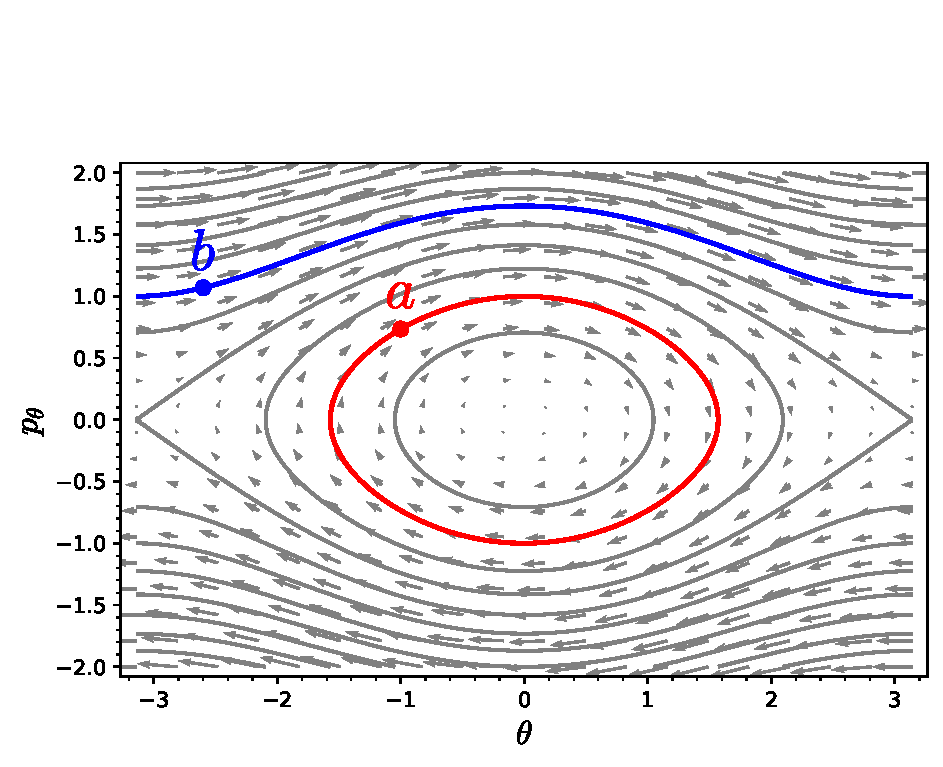
\includegraphics[width=0.8\textwidth]{evo_pendulum_phase.pdf}}
\caption[]{\label{f:tha:pendulum_phase} \footnotesize
Phase space $\FF$ of a simple gravity pendulum, depicted in terms of the
canonical coordinates $(\th,p_\th)$ (cf. Example~\ref{x:tha:pendulum}).
The vertical lines $\th=-\pi$ and $\th=\pi$ must be identified,
since $\FF = \SS^1 \times \mathbb{R}$.
The grey arrows show the Hamiltonian vector field $X_H$ and the grey
lines are some of its integral curves. Two of them are highlighted: the red
one corresponds to oscillating solutions ($\th$ having a limited range and $p_\th$ taking positive and negative values), while the blue one corresponds to solutions
rotating indefinitely in the anticlockwise direction ($p_\th>0$).
The points $a$ and $b$ each represent the initial data of a
given solution in these families; these points can also be viewed as defining
the solution itself (covariant phase space approach).}
\end{figure}

\begin{example}[phase space of a pendulum]
\label{x:tha:pendulum}
A simple gravity pendulum is a system with $N=1$, the unique degree of
freedom being the angle $\theta\in(-\pi,\pi]$ with respect to the vertical direction.
For a unit mass, the Lagrangian is
$L(\th,\dot{\th}) = (\ell\dot{\th})^2/2 + g \ell \cos\th$,
where $\ell$ is the length of the (massless) rod and $g$
the magnitude of the vertical gravity field. The momentum conjugate to $\th$
is $p_\th = \dert{L}{\dot{\th}} = \ell^2\dot{\th}$. Since the latter can
take any real value, the phase space $\FF$ is the 2-dimensional infinite cylinder
$\SS^1 \times \mathbb{R}$,
spanned by the canonical coordinates $(\th,p_\th)$. The
Hamiltonian is deduced from $L$ by the Legendre transform $H = p_\th \dot{\th} - L$,
yielding
$H(\theta,p_\theta) = p_\theta^2 / (2\ell^2) - g\ell\cos\theta$.
The Hamiltonian vector field is obtained via Eq.~(\ref{e:tha:X_f_canonical}):
$X_H = \ell^{-2} p_\th \, \partial_\th - g \ell \sin\th \, \partial_{p_\th}$.
It is depicted in Fig.~\ref{f:tha:pendulum_phase}.
\end{example}

%\begin{example}[phase space as the cotangent bundle of configuration space]
%In Example~\ref{x:tha:pendulum}, the space in which the degree of
%freedom $\theta$ evolves is the 1-dimensional manifold $\mathcal{C} = \mathbb{S}^1$.
%More generally, for a system of $N$ degrees of freedom, the space spanned by the
%latter is a $N$-dimensional manifold $\mathcal{C}$, called the
%\defin{configuration space}\index{configuration space}.
%\end{example}

Equation~(\ref{e:tha:Xf_Poisson_f}) with $f=H$
reads $\{. ,H\} = X_H$. Hence, for any scalar field $f$ on $\FF$,
$\{f,H\} = X_H(f)$ and the evolution law (\ref{e:tha:dfdt_Poisson_fH}) can be rewritten as
\be \label{e:tha:dfdt_X_H_f}
    \encadre{ \derd{f}{t} = X_H(f) }.
\ee
In particular, Hamilton's equations (\ref{e:evo_Hamilton_eqs_finite}) become
\be \label{e:evo_Hamilton_eqs_X_H}
    \derd{q^i}{t} = X_H(q^i) \qand \derd{p_i}{t} = X_H(p_i) , \quad 1 \leq i \leq N .
\ee
It follows that any solution $(q^i(t),p_i(t))$ to the equations of motion is an
integral curve of the Hamiltonian vector field in the phase space
(cf. Fig.~\ref{x:tha:pendulum}). $H$ is constant along such a curve, since,
from Eq.~(\ref{e:tha:DH_Omega_X_H}),
$X_H(H) = \langle \Dd H, X_H \rangle = \Omega(X_H, X_H) = 0$.

In view of Eq.~(\ref{e:tha:dfdt_X_H_f}), one may consider the vector field $X_H$ as
defining the ``time evolution'' without having to refer explicitely
to the time coordinate $t$.
Of course, we recover from Eq.~(\ref{e:tha:dfdt_X_H_f})
that $\D H/\D t = 0$ since $X_H(H) = 0$.
For tensor fields on $\FF$ of valence higher than a scalar field,
one  defines the ``time evolution'' as the
\emph{Lie derivative} $\Liesymbol_{X_H}$ along the Hamiltonian vector field $X_H$.
This is quite natural since the vanishing of $\Liesymbol_{X_H} T$ means
that the tensor field $T$ is transported identically to itself along the flow
defined by $X_H$ (cf. Sec.~\ref{s:bas:Lie}).
In particular, this encompasses Eq.~(\ref{e:tha:dfdt_X_H_f}), since
$\Liesymbol_{X_H} f = X_H(f)$ for any scalar field $f$.
An important feature of the evolution thus defined is that
the symplectic form is conserved:
\be \label{e:tha:Lie_X_H_Omega}
   \encadre{ \Liesymbol_{X_H} \Omega = 0 }.
\ee
\begin{proof}
The proof relies on the fact that $\Omega$ is closed, i.e. $\Dd\Omega = 0$.
Indeed, using successively the Cartan
identity (\ref{e:bas:Cartan}), Eq.~(\ref{e:tha:DH_Omega_X_H})
and the nilpotence property (\ref{e:ext_der_nilpot}), we get
\[
     \Liesymbol_{X_H} \Omega  = X_H \cdot \underbrace{\Dd \Omega}_{0}
     + \Dd(\underbrace{X_H\cdot\Omega}_{\Omega(X_H, .)})
     = - \Dd(\underbrace{\Omega(., X_H)}_{\Dd H})
     = - \Dd \Dd H = 0 .
\]
\end{proof}

Let us summarize the above results as follows:

\begin{prop}[Hamiltonian system]
\label{p:tha:Hamiltonian_system}
A \defin{Hamiltonian system}\index{Hamiltonian!system}
is a triplet $(\FF,\Omega,H)$ where $\FF$ is a smooth
manifold, called the \defin{phase space}\index{phase space} of the system, $\Omega$ is
a \defin{symplectic form}\index{symplectic!form} on $\FF$, i.e. a closed non-degenerate
2-form, and $H$ is a smooth function $\FF \to \R$ called
the \defin{Hamiltonian}.
The differential $\Dd H$ of $H$ is a 1-form  on
$\FF$, whose symplectic dual defines
the \defin{Hamiltonian vector field}\index{Hamiltonian!vector field},
namely the unique vector field $X_H$
on $\FF$ such that
\be \label{e:tha:DH_Omega_X_H_2}
\encadre{ \Dd H = \Omega(., X_H) }.
\ee
By construction, $X_H$ preserves the symplectic
form: $\Liesymbol_{X_H} \Omega = 0$ [Eq.~(\ref{e:tha:Lie_X_H_Omega})].
The evolution of the underlying physical system is entirely determined
by the Hamiltonian vector field: any solution to the equations of motion
is an integral curve of $X_H$.
A smooth function $f: \ \FF \to \R$ is called a
\defin{conserved quantity}\index{conserved!quantity} iff $f$ is constant on every integral curve
of $X_H$, i.e. iff $X_H(f) = 0$. In view of Eq.~(\ref{e:tha:crochet_Poisson_equiv}),
this is equivalent to $\{f,H\} = 0$.
A conserved quantity is $H$ itself. Its value for a given solution to the equations of motion
is called the \defin{energy}\index{energy!in Hamiltonian framework} of the solution.
An \defin{equilibrium point} is a point of $\FF$ where $X_H = 0$,
or equivalently, given Eq.~(\ref{e:tha:DH_Omega_X_H_2}), a point where
$\Dd H = 0$.
\end{prop}

\begin{example}[solutions for the gravity pendulum]
For the gravity pendulum considered in Example~\ref{x:tha:pendulum},
the integral curves of $X_H$ are depicted in Fig.~\ref{f:tha:pendulum_phase}.
Two of them are
represented by the red and the blue curves. It is clear from the figure
that $X_H$ vanishes at two points: $(\th,p_\th) = (0,0)$ and $(\th,p_\th) = (\pi,0)$,
which are thus two equilibrium points (respectively stable and unstable).
\end{example}


\begin{remark}
\label{r:tha:Ham_syst_no_canonical_coord}
The above formulation of Hamiltonian systems does not
refer to any system of canonical coordinates $(q^i, p_i)$ on
the phase space $\FF$
and, more generally, to any kind of coordinates.
It does not even assume that $\FF$ is the cotangent bundle $T^*\mathcal{C}$
of some ``configuration space'' $\mathcal{C}$,
while the cotangent bundle\index{cotangent bundle} structure is the standard
arena for the Hamiltonian mechanics with a finite number of degrees
of freedom \cite{AbrahM78}.
\end{remark}

\subsection{Covariant phase space}

Despite Remark~\ref{r:tha:Ham_syst_no_canonical_coord}, the Hamiltonian formulation sketched in
Property~\ref{p:tha:Hamiltonian_system} is not fully covariant.
Indeed, via the Hamiltonian
vector field $X_H$, it describes the evolution of the system with
respect to some ``privileged time'' $t$ [cf. Eq.~(\ref{e:tha:dfdt_X_H_f})].
To treat covariantly relativistic systems, it would be desirable to get
rid of the choice of a time function. This can be acheived as follows.

There is one, and exactly one,
integral curve of $X_H$ through each point\footnote{At an equilibrium point, the
integral curve is reduced to the point itself.} of $\FF$.
It follows that a solution is entirely determined by a single point $a\in\FF$,
which can be thought of as representing the state of the system at some initial
instant $t=t_0$, i.e. the coordinates of $a$ are $(q^i(t_0),p_i(t_0))$
(cf. Fig.~\ref{f:tha:pendulum_phase}).
If the initial value problem is well posed, there is a one-to-one
correspondance between a point of $\FF$ and a solution.
Consequently, one may view $\FF$ as the \emph{space of solutions}
to the equations of motion.
This is the essence of the
so-called \emph{covariant phase space}\index{covariant!phase space}\index{phase space!covariant --} approach:

\begin{prop}[covariant phase space]
\label{p:tha:cov_phase_space}
Let $(\FF,\Omega,H)$ be a Hamiltonian system whose
equations of motion constitute a well
posed initial value problem. Each solution to the equations of motion
is a curve $S: \R \to \FF$, $t\mapsto S(t)$, which admits the
Hamiltonian vector field $X_H$ as tangent vector.
The set $\FF_{\rm sol}$ of all solutions
can be given the structure of a smooth manifold diffeomorphic to $\FF$,
and for each $t_0\in \R$, an explicit diffeomorphism is
the ``initial data'' map
\be
    \begin{array}{rccl}
    \Phi_{t_0}: & \FF_{\rm sol} & \longrightarrow & \FF \\
        & S & \longmapsto & S(t_0) .
    \end{array}
\ee
Moreover, the pullback of the symplectic form $\Omega$ by $\Phi_{t_0}$,
\be \label{e:tha:Omega_sol_pullback}
    \Omega_{\rm sol} := \Phi_{t_0}^* \Omega ,
\ee
defines a symplectic form on $\FF_{\rm sol}$, which
is actually independent of $t_0$. This makes $(\FF_{\rm sol},\Omega_{\rm sol})$
a well-defined symplectic manifold, called the \defin{covariant phase space}\index{covariant!phase space}\index{phase space!covariant --}
of the system.
Infinitesimal displacement vectors on the manifold $\FF_{\rm sol}$
correspond to infinitesimal variations $\delta S$ between solutions,
so that Eq.~(\ref{e:tha:Omega_sol_pullback}) is equivalent to
\be \label{e:tha:Omega_sol_explicit}
    \Omega_{\rm sol}(\delta_1 S, \delta_2 S) :=
    \Omega\left(\overrightarrow{S(t_0)S_1(t_0)},\; \overrightarrow{S(t_0)S_2(t_0)} \right) ,
\ee
where $S$, $S_1 = S+\delta_1 S$ and $S_2 = S+\delta_2 S$ stand for three
nearby solutions.

Similarly, the pullback of the Hamiltonian $H$ by $\Phi_{t_0}$, i.e
$H_{\rm sol} := H \circ \Phi_{t_0}$, or equivalently,
\be \label{e:tha:def_H_sol}
    H_{\rm sol}(S) := H(S(t_0)) ,
\ee
defines a scalar field $H_{\rm sol}$
on $\FF_{\rm sol}$, which is independent of the choice of $t_0$.
\end{prop}
\begin{proof}
The equivalence between Eqs.~(\ref{e:tha:Omega_sol_pullback}) and (\ref{e:tha:Omega_sol_explicit}) follows readily from the definition of the pullback
map given in Sec.~\ref{s:bas:push_pull}. The independence
of $\Omega_{\rm sol}(\delta_1 S, \delta_2 S)$ from the choice of $t_0$
follows from the constancy of $\Omega$ along the Hamiltonian flow, i.e.
Eq.~(\ref{e:tha:Lie_X_H_Omega}). Indeed $\Omega_{\rm sol}(\delta_1 S, \delta_2 S)$,
as defined by Eq.~(\ref{e:tha:Omega_sol_explicit}), is independent of $t_0$
iff $\D f / \D t = 0$, where
$f(t) := \Omega (Y_1(t), Y_2(t))$
and we have introduced the separation vectors $Y_1(t) := \overrightarrow{S(t)S_1(t)}$ and $Y_2(t) := \overrightarrow{S(t)S_2(t)}$. Now, from Eq.~(\ref{e:tha:dfdt_X_H_f})
and the Leibniz rule,
\[
    \derd{f}{t} = \Liesymbol_{X_H} f
    = \Liesymbol_{X_H} \left[ \Omega (Y_1, Y_2) \right]
    = \underbrace{\Liesymbol_{X_H} \Omega}_{0} \,  (Y_1, Y_2)
        + \Omega( \underbrace{\Liesymbol_{X_H} Y_1}_{0}, \, Y_2 )
        + \Omega(  Y_1,\,  \underbrace{\Liesymbol_{X_H} Y_2}_{0} )
    = 0,
\]
where $\Liesymbol_{X_H} \Omega = 0$ is the invariance property (\ref{e:tha:Lie_X_H_Omega})
and $\Liesymbol_{X_H} Y_1 = 0$ and $\Liesymbol_{X_H} Y_2 = 0$ follows from the very definition
of a Lie derivative (cf. Sec.~\ref{s:bas:Lie}),
the separation vectors $Y_1$ and $Y_2$ being naturally Lie-dragged by $X_H$.
Finally, the independence of $H_{\rm sol}$ from the choice of $t_0$
is immediate from Eq.~(\ref{e:tha:def_H_sol}), which shows that
$H_{\rm sol}(S)$ is the energy of the solution $S$
(cf. Property~\ref{p:tha:Hamiltonian_system}).
\end{proof}

The triplet $(\FF_{\rm sol}, \Omega_{\rm sol}, H_{\rm sol})$ clearly constitutes
a Hamiltonian system, as defined in Property~\ref{p:tha:Hamiltonian_system}, but
without reference to any ``time evolution'', given that each point $S\in\FF_{\rm sol}$
is a fully evolved solution by itself. The fully covariant picture is thus achieved.
The Hamiltonian vector field $X_{H_{\rm sol}}$ is a vector field on $\FF_{\rm sol}$,
which generates 1-dimensional families of solutions. Two solutions $S_1$ and $S_2$
that lie on the same integral curve of $X_{H_{\rm sol}}$ are then
solutions to the original equations of motion that only differ by a time translation,
i.e. $S_2(t) = S_1(t + t_0)$ for some $t_0\in\R$. In particular $S_1$ and $S_2$
have the same energy.



\subsection{Covariant phase space for gravity theories} \label{s:tha:cps_gravity}

In order to apply the covariant phase space approach to
a gravity theory governed by a Lagrangian of the type (\ref{e:tha:Lagrangian_diffeo_inv}),
let us consider the
space $\FF_{\rm sol}$ of solutions $\w{g}$ to the field equations
(\ref{e:tha:eom_E}). Since no confusion may arise, for simplicity,
we shall drop the index ``sol'' and denote this space simply by\footnote{Be aware that in
some part of the
literature \cite{AshteBR91,LeeW90,WaldZ00}, $\FF$ denotes instead the space of all fields $\w{g}$
that are required to only obey some asymptotic flatness conditions, but not necessarily the field equations;
the subspace of solutions to the field equations --- our $\FF$ --- is then denoted
by $\bar{\FF}$ \cite{LeeW90,WaldZ00} or $\Gamma$ \cite{AshteBR91}.} $\FF$.
A difference with what precedes is that
we are dealing with a field theory, which, by essence, has
an infinite number of degrees of freedom. In other words,
the space of solutions $\FF$ is
an \emph{infinite-dimensional manifold}. More precisely, it can be given the structure of an
infinite-dimensional \defin{Banach manifold}\index{Banach manifold}\index{manifold!Banach --}
\cite{LeeW90,HarloW20}, i.e. a topological space that locally resembles\footnote{Cf. Lang's book~\cite{Lang95} for a
precise definition of a Banach manifold.} a Banach space of infinite dimension, in the same
way as a $n$-dimensional manifold locally resembles the vector space $\mathbb{R}^n$.
Since any point of $\FF$ is a metric field $\w{g}$ on $\M$, a variation $\delta\w{g}$
can be viewed as an infinitesimal displacement vector between two neighboring points of the manifold
$\FF$, similar to the displacement vector $\D\w{x}$ on $\M$ introduced in Secs.~\ref{s:fra:general_settings} and \ref{s:bas:vectors}.
As in the finite dimensional case
(cf. Sec.~\ref{s:bas:vectors}), (non-infinitesimal) vectors on $\FF$
are defined\footnote{Notice that the definition (\ref{e:bas:def_vector}) of a tangent vector
does not require the manifold to be of finite dimension.} as tangent vectors
along \emph{curves of} $\FF$, the latter being the images of smooth maps
$P: I\subset \R \to  \FF$, $\lambda\mapsto P(\lambda) =: \w{g}(\lambda)$. Here
$\w{g}(\lambda)$ stands for a 1-parameter family of metric fields
on $\M$, this family constituting a parametrization of a given curve $\mathcal{L}$ of $\FF$.
Any vector $X$ at a point $\w{g}_0 \in \FF$ can then be written as in Eq.~(\ref{e:bas:dell_v_dlamb}):
\be \label{e:tha:X_dg/dlambda}
    X = \frac{\delta\w{g}}{\delta\lambda} ,
\ee
where $\delta\w{g}$ is the infinitesimal displacement vector connecting $\w{g}_0 =: \w{g}(\lambda)$
and $\w{g}(\lambda+\delta\lambda)$ along the curve $\mathcal{L}$
to which $X$ is tangent to; $\lambda$ is then the parameter of $\mathcal{L}$ associated to $X$
and we denote by $\delta\lambda$ its small increment, instead of $\D\lambda$ as in Sec.~\ref{s:bas:vectors}.


\begin{prop}[space of asymptotically flat solutions]
\label{p:tha:asymp_flat_sol}
In what follows, we assume that the $n$-dimensional spacetime manifold $\M$ is diffeomorphic to $\R\times\hat{\Sigma}$,
where $\hat{\Sigma}$ is an orientable manifold of dimension $(n-1)$ with an
\defin{asymptotically Euclidean end}\index{asymptotically!Euclidean end},
i.e. there exists a compact subset $K$ of $\hat{\Sigma}$ such that
$\hat{\Sigma}_{\rm ext} := \hat{\Sigma}\setminus K$
is diffeomorphic to $\R^{n-1} \setminus \mathbb{B}^{n-1}$, where $\mathbb{B}^{n-1}$ is the unit ball of
$\R^{n-1}$. Furthermore,
given two points $p$ and $p'$ in $\M$, we shall say that $p'$ lies in the
\defin{background future}\index{background!future}\index{future!background --} of $p$ iff for any orientation-preserving diffeomorphism $\Psi: \M \to \R\times \hat{\Sigma}$,
$\Psi(p') = (t', q')$ and $\Psi(p) = (t, q)$ with $t'>t$.

We shall restrict the space $\FF$ of solutions $\w{g}$ of the considered gravity theory
to those that are asymptotically flat, with the asymptotically flat end corresponding to
$\hat{\Sigma}_{\rm ext}$. The precise definition of \defin{asymptotically flat}\index{asymptotically!flat}\index{flat!asymptotically --} depends on the gravity theory
and should be such that some integrals indicated below converge and that
the asymptotic limit of some surface integrals is zero.
\end{prop}

We are going to see that, from the action (\ref{e:tha:action_L}),
we can endow $\FF$ with a (pre)symplectic form $\Omega$.
Let
$\Sigma$ and $\Sigma'$ be two non-intersectic hypersurfaces of $\M$,
both diffeomorphic to $\hat{\Sigma}$ and such that $\Sigma'$ lies in the
background future of $\Sigma$. Let $\Sigma_r$ and $\Sigma'_r$
be compact subparts
of $\Sigma$ and $\Sigma'$ respectively,
extending in the asymptotic flat end and corresponding to balls of Euclidean radius $r$
in $\hat{\Sigma}_{\rm ext}$. Let $\mathscr{W}_r$
be the hypercylinder
connecting $\Sigma_r$ to $\Sigma'_r$ (cf. Fig.~??)
and $\mathscr{D}$ be the part
of $\M$ bounded by $\Sigma_r$, $\Sigma'_r$ and $\mathscr{W}_r$. Let us then consider the
action (\ref{e:tha:action_L}) restricted to $\mathscr{D}$:
\be \label{e:tha:def_action_S_D}
    \mathcal{S}_{\mathscr{D}}[\w{g}] := \int_{\mathscr{D}} \w{L}\lld\w{g}\rld .
\ee
We are using the \emph{functional} notation $\mathcal{S}_{\mathscr{D}}[\w{g}]$,
but, when restricted to solutions $\w{g}$ of the field equations,
$\mathcal{S}_{\mathscr{D}}$ is merely a scalar field on the manifold $\FF$,
i.e. a \emph{function} $\FF\to \R$.
Accordingly, the variation $\delta\mathcal{S}_{\mathscr{D}}$ of $\mathcal{S}_{\mathscr{D}}$
due to a small displacement $\delta\w{g}$ on $\FF$ can be viewed
as the action of the differential 1-form $\Dd \mathcal{S}_{\mathscr{D}}$
on the infinitesimal vector $\delta\w{g}$:
$\delta\mathcal{S}_{\mathscr{D}} =
\langle \Dd \mathcal{S}_{\mathscr{D}},\delta\w{g}\rangle$
[cf. Eq.~(\ref{e:bas:df})]. Now, from the definition~(\ref{e:tha:def_action_S_D}),
we get $\delta\mathcal{S}_{\mathscr{D}} = \int_{\mathscr{D}} \delta \w{L}\lld\w{g}\rld$,
with $\delta\w{L}\lld\w{g}\rld$ given by Eq.~(\ref{e:tha:delta_L_E_Theta}),
in which $\w{E}$ is set to zero for elements of $\FF$ are solutions of the field equations.
Hence
$\langle \Dd \mathcal{S}_{\mathscr{D}},\delta\w{g}\rangle =
\int_{\mathscr{D}} \dd \w{\theta}\lld\w{g},\delta\w{g}\rld$.
By linearity\footnote{Recall that $\w{\theta}\lld\w{g},\delta\w{g}\rld$ is linear
with respect to $\delta\w{g}$, cf. Property~\ref{p:tha:var_Lagrangian}.}, we get for any vector $X = \delta\w{g}/\delta\lambda$ at a point $\w{g}\in\FF$,
\[
    \langle \Dd \mathcal{S}_{\mathscr{D}}, X\rangle =
\int_{\mathscr{D}} \dd \w{\theta}\Lld\w{g},\frac{\delta\w{g}}{\delta\lambda}\Rld .
\]
Thanks to Stokes' theorem (\ref{e:bas:Stokes}),
we rewrite the right-hand side as a surface integral, taking into
account that $\partial\mathscr{D} = \Sigma'_r \cup \Sigma_r \cup \mathscr{W}_r$:
\be \label{e:tha:dS_D_3int}
 \langle \Dd \mathcal{S}_{\mathscr{D}}, X\rangle =
\int_{{\Sigma'_r}^{\nearrow}} \w{\theta}\Lld\w{g},\frac{\delta\w{g}}{\delta\lambda}\Rld
+ \int_{\Sigma_r^{\nearrow}} \w{\theta}\Lld\w{g},\frac{\delta\w{g}}{\delta\lambda}\Rld
+ \int_{\mathscr{W}_r^{\nearrow}}
    \w{\theta}\Lld\w{g},\frac{\delta\w{g}}{\delta\lambda}\Rld ,
\ee
where the arrows indicate the outward orientation of the various hypersurfaces
with respect to $\mathscr{D}$.
Since Eq.~(\ref{e:tha:dS_D_3int}) is valid for any vector $X$ on $\FF$, we may rewrite
it as an identity between 1-forms:
\be \label{e:tha:dS_D_Theta_Upsilon}
    \Dd \mathcal{S}_{\mathscr{D}} = \Theta_{\Sigma'_r} - \Theta_{\Sigma_r}
    + \Upsilon_{\Sigma_r,\Sigma'_r} .
\ee
Here $\Theta_{\Sigma_r}$ stands the 1-form on $\FF$ defined by
the following action on a vector $X$ in the
tangent space $T_{\w{g}} \FF$:
\be \label{e:tha:def_Theta_X_theta}
    \langle \Theta_{\Sigma_r}, X \rangle := \int_{\Sigma_r} \w{\theta}\Lld\w{g},\frac{\delta\w{g}}{\delta\lambda}\Rld ,
\ee
where $\delta\w{g}/\delta\lambda$ is the relative variation of $\w{g}$ defining the
vector $X$ by Eq.~(\ref{e:tha:X_dg/dlambda}) and the orientation of $\Sigma_r$
is that provided by any background-future directed vector transverse to $\Sigma_r$.
Note that $\Theta_{\Sigma_r}$ is well defined, i.e. the integral in Eq.~(\ref{e:tha:def_Theta_X_theta}) is finite, because $\Sigma_r$ is compact
and $\w{\theta}$ is smooth; moreover, $\Theta_{\Sigma_r}$ is
linear for $\w{\theta}\lld\cdot,\cdot\rld$ is linear in its second argument.
The same definition holds for $\Theta_{\Sigma'_r}$.
Similarly, $\Upsilon_{\Sigma_r,\Sigma'_r}$ stands for the 1-form on $\FF$ defined
by
\be \label{e:tha:def_Upsilon}
    \langle \Upsilon_{\Sigma_r,\Sigma'_r}, X \rangle :=
    \int_{\mathscr{W}_r^{\nearrow}} \w{\theta}\Lld\w{g},\frac{\delta\w{g}}{\delta\lambda}\Rld ,
\ee
with $\mathscr{W}_r$ defined as above.
Note that the minus sign in front of $\Theta_{\Sigma_r}$ in Eq.~(\ref{e:tha:dS_D_Theta_Upsilon}) occurs because of the change
of orientation of $\Sigma_r$ between Eqs.~(\ref{e:tha:dS_D_3int}) and (\ref{e:tha:dS_D_Theta_Upsilon}).

In an attempt to endow $\FF$ with a symplectic form, thereby turning it into a phase space,
let us consider the 2-form $\Omega$ that is the limit $\Sigma_r \to \Sigma$
(i.e. the limit $r\to +\infty$) of the exterior derivative of $\Theta_{\Sigma_r}$.
This defines a closed 2-form, which turns out to be independent of
the choice of $\Sigma$:

\begin{prop}[presymplectic form in the space of solutions of a gravity theory]
\label{p:tha:presymplectic_form}
Let $\FF$ be the (Banach) manifold of solutions $\w{g}$ to the field equations
that are asymptotically flat in the asymptotically Euclidean end of the
$n$-dimensional manifold $\M \sim \R \times \hat{\Sigma}$. Let
$\Sigma$ be a hypersurface of $\M$ diffeomorphic to $\hat{\Sigma}$
and $\Sigma_r$ a compact subpart
of $\Sigma$ corresponding to a ball of Euclidean radius $r$
in $\hat{\Sigma}_{\rm ext}$.
Given the 1-form $\Theta_{\Sigma_r}$ defined on $\FF$ by Eq.~(\ref{e:tha:def_Theta_X_theta}),
the asymptotically flatness conditions of the gravity theory must insure that the limit
\be \label{e:tha:def_Omega_gravity}
   \encadre{ \Omega := \lim_{r\to +\infty} \Dd \Theta_{\Sigma_r} },
\ee
is well defined, i.e. yields a finite 2-form on $\FF$. This 2-form is closed:
$\Dd\Omega = 0$. One then says that $\Omega$ is a
\defin{presymplectic form}\index{presymplectic!form}\footnote{Recall that a \emph{symplectic form} is a 2-form that is closed \emph{and} non-degenerate; as we shall discuss
below, $\Omega$ is actually degenerate.} on $\FF$.
Moreover, $\Omega$ does not depend on the choice of the hypersurface $\Sigma$.
The pair $(\FF,\Omega)$ is called the \defin{prephase space}\index{prephase space} of the considered gravity theory
(and asymptotic flatness conditions).
\end{prop}

\begin{proof}
For each value of $r$, $\Dd \Theta_{\Sigma_r}$ is a 2-form on $\FF$, so if the
limit (\ref{e:tha:def_Omega_gravity}) exists, it clearly defines a 2-form
$\Omega$ on $\FF$.
Let us evaluate its exterior derivative, $\Dd \Omega$, by means of formula
(\ref{e:bas:def_ext_der}) with $p=2$: for any 3-tuple $(X_1,X_2,X_3)$ of
vector fields on $\FF$, we have
$\Dd\Omega(X_1,X_2,X_3) = X_1(\Omega(X_2,X_3)) -  X_2(\Omega(X_1,X_3))
+  X_3(\Omega(X_1,X_2)) - \Omega([X_1,X_2], X_3) + \Omega([X_1,X_3], X_2)
- \Omega([X_2,X_3], X_1)$.
Now
\[
X_1(\Omega(X_2,X_3)) = X_1 \left( \lim_{r\to +\infty} \Dd \Theta_{\Sigma_r}(X_2,X_3) \right)
    = \lim_{r\to +\infty}  X_1 \left( \Dd \Theta_{\Sigma_r}(X_2,X_3) \right) ,
\]
with similar formulas for $X_2(\Omega(X_1,X_3))$ and $X_3(\Omega(X_1,X_2))$.
There comes then
$\Dd\Omega(X_1,X_2,X_3) =
    \lim_{r \to \infty} \Dd \Dd \Theta_{\Sigma_r}(X_1,X_2,X_3)$.
But $\Dd \Dd \Theta_{\Sigma_r} = 0$ (nilpotence of the exterior
derivative, cf. Eq.~(\ref{e:ext_der_nilpot})). We conclude that $\Dd\Omega = 0$.
As for the independence of $\Omega$ from $\Sigma$, it arises from the following
identity obtained by taking the exterior derive of Eq.~(\ref{e:tha:dS_D_Theta_Upsilon})
and using $\Dd\Dd \mathcal{S}_{\mathscr{D}} = 0$
in the left-hand side:
\[
    0 = \Dd \Theta_{\Sigma'_r} - \Dd \Theta_{\Sigma_r}
    + \Dd \Upsilon_{\Sigma_r,\Sigma'_r} .
\]
Taking the limit $r\to +\infty$ yields
$\displaystyle \Omega_{\Sigma'} - \Omega_\Sigma  + \lim_{r\to+\infty} \Dd \Upsilon_{\Sigma_r,\Sigma'_r} = 0$.
The asymptotic flatness conditions
ensure that $\displaystyle\lim_{r\to+\infty} \Dd \Upsilon_{\Sigma_r,\Sigma'_r} = 0$ (Lemma~\ref{p:tha:Upsilon_closed} below),
leaving us with $\Omega_{\Sigma'} = \Omega_{\Sigma}$.
\end{proof}

\begin{remark}
Instead of the limit~(\ref{e:tha:def_Omega_gravity}),
it could have seemed simpler to define the presymplectic form
as $\Omega := \Dd\Theta_{\Sigma}$, where
$\Theta_{\Sigma}$ is defined as in Eq.~(\ref{e:tha:def_Theta_X_theta}) but with the
integral extended to the whole of $\Sigma$. However, as noticed in Ref.~\cite{AshteBR91} (p.~429), standard asymptotic flatness conditions
do not guarantee that this integral is convergent; hence the 1-form $\Theta_{\Sigma}$ would be ill-defined.
\end{remark}


\begin{prop}[presymplectic current $(n-1)$-form]
\label{p:tha:presymplectic_current}
The action of the presymplectic form $\Omega$ on a pair of commuting vector fields $(X_1,X_2)$ of $\FF$
is expressible as follows.
According to Eq.~(\ref{e:tha:X_dg/dlambda}),
each vector field describes the variation of $\w{g}$ along some curves of $\FF$.
Since they commute, the vector fields $(X_1,X_2)$ can be associated
to a 2-parameter family $\w{g}(\lambda_1,\lambda_2)$ of metric tensors,
spanning a 2-surface $\mathcal{S}\subset \FF$, so that $X_1$
(resp. $X_2$) corresponds to variations
$\delta\w{g}$
along curves $\lambda_2 = \mathrm{const}$ (resp. $\lambda_1 = \mathrm{const}$) in the 2-surface $\mathcal{S}$, i.e. to partial derivatives:
\be \label{e:tha:def_X1_X2}
    X_1 = \left. \frac{\delta\w{g}}{\delta\lambda_1} \right| _{\lambda_2=\mathrm{const}}
      =: \der{\w{g}}{\lambda_1}  \qand
    X_2 = \left. \frac{\delta\w{g}}{\delta\lambda_2} \right| _{\lambda_1=\mathrm{const}}
      =: \der{\w{g}}{\lambda_2} .
\ee
We have then
\be \label{e:tha:Omega_int_omega}
    \encadre{ \Omega(X_1,X_2) =  \int_{\Sigma} \w{\omega}\Lld\w{g},  \der{\w{g}}{\lambda_1},
                            \der{\w{g}}{\lambda_2} \Rld } ,
\ee
where $\w{\omega}$ is the $(n-1)$-form on $\M$ defined from the
presymplectic potential $(n-1)$-form $\w{\theta}$
of the considered gravity theory
(cf. Property~\ref{p:tha:var_Lagrangian}) by
\be \label{e:tha:def_omega_der_theta}
 \encadre{ \w{\omega}\Lld\w{g},  \der{\w{g}}{\lambda_1}, \der{\w{g}}{\lambda_2} \Rld
    :=  \der{}{\lambda_1}
        \left( \w{\theta}\Lld\w{g}, \der{\w{g}}{\lambda_2} \Rld\right)
        - \der{}{\lambda_2}\left( \w{\theta}\Lld\w{g}, \der{\w{g}}{\lambda_1} \Rld \right) } .
\ee
$\w{\omega}$ is called the
\defin{presymplectic current $(n-1)$-form}\index{presymplectic!current form}
\cite{WaldZ00}\footnote{It is called the \emph{symplectic current $(n-1)$-form}
in articles by Wald and Iyer \cite{Wald93,IyerW94} preceding \cite{WaldZ00}, but, as
discussed below, \emph{presymplectic} is a better qualifier than \emph{symplectic}.}.
It has a local dependence on the metric tensor $\w{g}$
and on the derivatives $\dert{\w{g}}{\lambda_1}$ and $\dert{\w{g}}{\lambda_2}$
associated to the 2-parameter family $\w{g}(\lambda_1,\lambda_2)$,
and is linear with respect to these derivatives.
\end{prop}

\begin{proof}
Let us compute $\Dd \Theta_{\Sigma_r} (X_1,X_2)$ via the exterior derivative formula
(\ref{e:bas:def_ext_der_p1}), noticing that (i) this formula
does not involve the manifold dimensionality (contrary to (\ref{e:bas:def_ext_1f}),
which applies to finite dimensions only) and (ii) the last term in the right-hand
side of (\ref{e:bas:def_ext_der_p1}) vanishes since $[X_1,X_2] = 0$.
We get
\begin{align}
    \Dd \Theta_{\Sigma_r} (X_1,X_2) & = X_1\left( \langle \Theta_{\Sigma_r}, X_2 \rangle \right)
        -  X_2\left( \langle \Theta_{\Sigma_r}, X_1 \rangle \right) \nonumber \\
        & =  \der{}{\lambda_1} \langle \Theta_{\Sigma_r}, X_2 \rangle -
            \der{}{\lambda_2} \langle \Theta_{\Sigma_r}, X_1 \rangle \nonumber \\
        & = \der{}{\lambda_1} \int_{\Sigma_r} \w{\theta}\Lld\w{g}, \der{\w{g}}{\lambda_2} \Rld
        - \der{}{\lambda_2} \int_{\Sigma_r} \w{\theta}\Lld\w{g}, \der{\w{g}}{\lambda_1} \Rld   \nonumber \\
        & = \int_{\Sigma_r} \left\{ \der{}{\lambda_1}
        \left( \w{\theta} \Lld\w{g}, \der{\w{g}}{\lambda_2} \Rld \right)
        - \der{}{\lambda_2}\left( \w{\theta}\Lld\w{g}, \der{\w{g}}{\lambda_1} \Rld \right) \right\} .
        \nonumber
\end{align}
The second equality results from $X_1(f) = \dert{f}{\lambda_1}$ for the scalar field
$f := \langle \Theta_{\Sigma_r}, X_2 \rangle$ [cf. Eq.~(\ref{e:bas:def_vector})], the third equality
makes use of Eqs.~(\ref{e:tha:def_Theta_X_theta}) and (\ref{e:tha:def_X1_X2})
and the last equality stems from the linearity of the integral.
Since $\Omega(X_1,X_2) = \lim_{r\to+\infty} \Dd \Theta_{\Sigma_r} (X_1,X_2)$ and
$\Sigma_r \to \Sigma$ for $r\to+\infty$,
this proves Eq.~(\ref{e:tha:Omega_int_omega}), provided that
$\w{\omega}$ is defined by (\ref{e:tha:def_omega_der_theta}).
The $(n-1)$-form $\w{\omega}$ does not depend on the second derivative
$\frac{\partial^2\w{g}}{\partial\lambda_1\partial\lambda_2}$ because the second derivatives,
which appear in each of the two terms of the right-hand side of
Eq.~(\ref{e:tha:def_omega_der_theta}), cancel out thanks to the
identity
$\frac{\partial^2\w{g}}{\partial\lambda_1\partial\lambda_2} = \frac{\partial^2\w{g}}{\partial\lambda_2\partial\lambda_1}$.
Hence the notation $\w{\omega} = \w{\omega}\lld\w{g},  \dert{\w{g}}{\lambda_1}, \dert{\w{g}}{\lambda_2} \rld$.
\end{proof}

\begin{example}[presymplectic current form of general relativity]
For general relativity, one deduces from expression~(\ref{e:tha:Theta_GR})
for $\w{\theta}$ and the definition (\ref{e:tha:def_omega_der_theta}) that
the presymplectic current $(n-1)$-form is
\be
    \omega\lld \w{g}, \delta_1 \w{g}, \delta_2 \w{g} \rld _{\alpha_1\cdots\alpha_{n-1}} =
     (32\pi)^{-1}\, P^{\lambda\mu\nu\tau\rho\sigma}
    \left( \delta_2 g_{\mu\nu} \nabla_\tau \delta_1 g_{\rho\sigma}
    - \delta_1 g_{\mu\nu} \nabla_\tau \delta_2 g_{\rho\sigma} \right)
    \epsilon_{\lambda\alpha_1\cdots\alpha_{n-1}} ,
\ee
with
\be
    P^{\lambda\mu\nu\tau\rho\sigma}
    := 2 g^{\lambda\rho} g^{\sigma\mu} g^{\nu\tau}
       - g^{\lambda\tau} g^{\mu\rho} g^{\sigma\nu}
       - g^{\lambda\mu} g^{\nu\tau} g^{\rho\sigma}
       - g^{\mu\nu} g^{\lambda\rho} g^{\sigma\tau}
       + g^{\mu\nu} g^{\lambda\tau} g^{\rho\sigma} .
\ee
We shall not detail the computation, which is straightforward but rather lengthy.
Let us simply mention that one shall start by expressing the
covariant derivatives in formula~(\ref{e:tha:Theta_GR})
for $\w{\theta}$ in terms of $\w{g}$'s Christoffel symbols [Eq.~(\ref{e:bas:der_cov_coord})
with $(k,\ell) = (0,2)$] and replace $\weps$ by $\sqrt{-g}\, \w{e}$ as in Example~\ref{x:tha:theta_GR},
plug the result in Eq.~(\ref{e:tha:def_omega_der_theta}) and
make use of the identities
(\ref{e:evo:delta_Gamma}) and (\ref{e:evo:delta_sqrt_g}).
As a check, one can compare with
Eqs.~(21)-(23) of Ref.~\cite{HollaW13} or
Eqs.~(41)-(43) of Ref.~\cite{WaldZ00}.
\end{example}

\begin{lemma}[asymptotic vanishing of $\Dd \Upsilon_{\Sigma_r,\Sigma'_r}$]
\label{p:tha:Upsilon_closed}
The 1-form $\Upsilon_{\Sigma_r,\Sigma'_r}$ defined by Eq.~(\ref{e:tha:def_Upsilon})
obeys $\lim_{r\to+\infty} \Dd \Upsilon_{\Sigma_r,\Sigma'_r} = 0$.
\end{lemma}
\begin{proof}
By exactly the same computation as that leading to Eq.~(\ref{e:tha:Omega_int_omega}),
we have
\[
     \Dd \Upsilon_{\Sigma_r,\Sigma'_r}(X_1,X_2) =
      \int_{\mathscr{W}_r^{\nearrow}}
     \w{\omega}\Lld\w{g},  \der{\w{g}}{\lambda_1},
                            \der{\w{g}}{\lambda_2} \Rld .
\]
As argued in Ref.~\cite{IyerW94},
if the asymptotic flatness conditions ensure that the integral (\ref{e:tha:Omega_int_omega})
on the unbounded hypersurface $\Sigma$ is convergent, then the integral of
the same integrand $\w{\omega}$ over $\mathscr{W}_r$ must tend to zero for $r\to +\infty$.
\end{proof}



\begin{prop}[uniqueness of the presymplectic form]
\label{p:tha:uniqueness_presympl}
The presymplectic form $\Omega$ is unique for a given gravity theory with
appropriate asymptotic flatness conditions. Not only it is
does not depend on the choice of the
hypersurface $\Sigma$ (Property~\ref{p:tha:presymplectic_form}),
but it is unaffected by the ambiguities
$\w{\theta} \to \w{\theta} + \dd \w{Y} + \delta\w{\mu}$
in the definition of $\w{\theta}$ [cf. Eq.~(\ref{e:tha:Theta_not_unique})].
Moreover, the presymplectic current $(n-1)$-form $\w{\omega}$ itself is unaffected
by the ambiguity
$\w{\theta} \to \w{\theta} + \delta\w{\mu}$.
\end{prop}

\begin{proof}
Let us first show the last point, by evaluating $\w{\omega}$
from Eq.~(\ref{e:tha:def_omega_der_theta})
for $\w{\theta'}\lld\w{g},\delta\w{g}\rld = \w{\theta}\lld\w{g},\delta\w{g}\rld
+ \delta \w{\mu}\lld\w{g}\rld$.
For $\delta\w{g} = (\dert{\w{g}}{\lambda_2}) \, \delta \lambda_2$, we get
\[
\w{\theta'}\Lld\w{g}, \der{\w{g}}{\lambda_2} \Rld = \w{\theta}\Lld\w{g}, \der{\w{g}}{\lambda_2} \Rld + \der{}{\lambda_2} \w{\mu}\lld\w{g}\rld ,
\]
so that
\[
  \der{}{\lambda_1}
        \left( \w{\theta'}\Lld\w{g}, \der{\w{g}}{\lambda_2} \Rld\right)
    = \der{}{\lambda_1}
        \left( \w{\theta}\Lld\w{g}, \der{\w{g}}{\lambda_2} \Rld\right)
        + \frac{\partial^2}{\partial\lambda_1\partial\lambda_2} \w{\mu}\lld\w{g}\rld
 .
\]
Thanks to the commutativity of partial derivatives, the terms
involving $\w{\mu}$ cancel each other when substituting $\w{\theta'}$
for $\w{\theta}$ in Eq.~(\ref{e:tha:def_omega_der_theta}).
Hence the $(n-1)$-form $\w{\omega}$ computed from $\w{\theta'}$
is the same as that computed from $\w{\theta}$.
It follows then from Eq.~(\ref{e:tha:Omega_int_omega}) that
the presymplectic form $\Omega$ is independent of $\w{\mu}$ as well.
On the other side,
the change  $\w{\theta'}\lld\w{g},\delta\w{g}\rld = \w{\theta}\lld\w{g},\delta\w{g}\rld
+ \dd \left(\w{Y}\lld\w{g},\delta\w{g}\rld \right)$, as permitted by Eq.~(\ref{e:tha:Theta_not_unique}),
leads to the following change in the presymplectic form:
\[
    \Omega'(X_1, X_2) = \Omega(X_1, X_2) + \int_{\Sp_\infty}
    \left[ \der{}{\lambda_1}
        \left( \w{Y}\Lld\w{g}, \der{\w{g}}{\lambda_2} \Rld\right)
        - \der{}{\lambda_2}\left( \w{Y}\Lld\w{g}, \der{\w{g}}{\lambda_1} \Rld \right) \right] ,
\]
where use has been made of Eqs.~(\ref{e:tha:Omega_int_omega})-(\ref{e:tha:def_omega_der_theta}),
as well as the Stokes' theorem (\ref{e:bas:Stokes}),
$\Sp_\infty$ standing for the ``outer boundary'' of $\Sigma$, i.e. the limit
$r\to +\infty$ of a $(n-2)$-sphere $\Sp_r$ of radius $r$ in the asymptotically Euclidean end
of $\Sigma$. Now, given that the $(n-2)$ form $\w{Y}$ must be constructed from
$\w{g}$, $\delta\w{g}$ and their derivatives in a covariant manner, the fall-off
conditions from standard asymptotic flatness are sufficient to make
the above integral over $\Sp_\infty$ vanish \cite{IyerW94}. Hence $\Omega' = \Omega$.
\end{proof}


\begin{prop}[closedness of the presymplectic current $(n-1)$-form]
\label{p:tha:omega_closed}
Provided that the 2-parameter family $\w{g}(\lambda_1,\lambda_2)$
involved in the definition (\ref{e:tha:def_omega_der_theta}) regards
only solutions to the field equations (i.e. $\w{g}(\lambda_1,\lambda_2) \in \FF$),
the presymplectic current $\w{\omega}$ is a closed $(n-1)$-form:
\be \label{e:tha:omega_closed}
    \dd \w{\omega} = 0 .
\ee
\end{prop}
\begin{proof}
The 2-parameter family of metric tensors $\w{g}(\lambda_1,\lambda_2)$ gives birth
to a 2-parameter family of Lagrangian $n$-forms
$\w{L}(\lambda_1,\lambda_2) := \w{L}\lld\w{g}(\lambda_1,\lambda_2)\rld$.
The variation $\delta_1\w{L}$ of $\w{L}$ corresponding to a variation of $\lambda_1$ is
given by Eq.~(\ref{e:tha:delta_L_E_Theta}) with $E^{\mu\nu} = 0$ since
$\w{g}(\lambda_1,\lambda_2)$ fulfills the field equations. Hence
$\delta_1 \w{L} = \dd \left( \w{\theta}\lld\w{g}, \delta_1 \w{g}\rld \right)$.
Given that $\delta_1 \w{L} = \der{\w{L}}{\lambda_1}  \, \delta \lambda_1$,
$\delta_1 \w{g} = \der{\w{g}}{\lambda_1} \, \delta \lambda_1$
and $\w{\theta}\lld .,.\rld$ is linear with respect to its second argument, we get
$\dert{\w{L}}{\lambda_1} = \dd \left( \w{\theta} \lld\w{g},  \dert{\w{g}}{\lambda_1} \rld \right)$.
%\[
%    \der{\w{L}}{\lambda_1} = \dd \left( \w{\theta} \Lld\w{g},  \der{\w{g}}{\lambda_1} \Rld \right) .
%\]
Taking the derivative of this expression with respect to $\lambda_2$ yields
\[
    \frac{\partial^2\w{L}}{\partial\lambda_2\partial\lambda_1} = \der{}{\lambda_2}
        \dd \left( \w{\theta} \Lld\w{g},  \der{\w{g}}{\lambda_1} \Rld \right)
        = \dd  \der{}{\lambda_2} \left( \w{\theta} \Lld\w{g},  \der{\w{g}}{\lambda_1} \Rld \right) .
\]
Swapping $\lambda_1$ and $\lambda_2$ and subtracting the above formula
yields, in view of $\w{\omega}$'s definition (\ref{e:tha:def_omega_der_theta}),
$\frac{\partial^2\w{L}}{\partial\lambda_1\partial\lambda_2} - \frac{\partial^2\w{L}}{\partial\lambda_2\partial\lambda_1} = \dd\w{\omega}$. But the left-hand side of this equation
is trivially zero, hence the result (\ref{e:tha:omega_closed}).
\end{proof}

It turns out that in general, the presymplectic form $\Omega$
is \emph{degenerate}:
there exists nonzero vectors $X$ on $\FF$, such that $\Omega(X,.) = 0$.
Hence $\Omega$ fails to be a symplectic form on $\FF$.
For instance, one may conceive a nonzero variation $\delta\w{g}$
of $\w{g}$ such that $\delta\w{g} = 0$ on the hypersurface $\Sigma$ involved
in Eq.~(\ref{e:tha:Omega_int_omega}). Then, by linearity of
$\w{\omega}\lld\w{g},\delta_1\w{g},\delta_2\w{g}\rld$ with respect to
$\delta_1\w{g}$ and $\delta_2\w{g}$ (cf. Property~\ref{p:tha:presymplectic_current}), one has
$\w{\omega}\lld\w{g},\delta\w{g},.\rld = 0$ on $\Sigma$
and Eq.~(\ref{e:tha:Omega_int_omega}) shows that $\delta\w{g}$ defines
a degeneracy direction of $\Omega$. More generally, the degeneracy of $\Omega$
is related to the gauge freedom of the gravity theory, i.e. to the
invariance by diffeomorphism. For general relativity, it has been shown
\cite{AshteBR91} that the degeneracy directions of $\Omega$ are exactly
those generated by diffeomorphisms of $\M$ [cf.
Eqs.~(\ref{e:tha:delta_g_Phistar})-(\ref{e:bas:delta_g_Lie_xi_g})] that reduce to the identity at infinity
(i.e. such that $\w{\xi}$ in Eq.~(\ref{e:bas:delta_g_Lie_xi_g}) tends to
zero for $r\to +\infty$). The gauge freedom is intimately related to the
initial value problem of the theory being \emph{not} well posed (it becomes
well posed only in a fixed gauge, see e.g. Chap.~VI of Ref.~\cite{Choqu09}). Recall that in the covariant phase space
construction of Property~\ref{p:tha:cov_phase_space}, it was required
that the initial value problem is well posed to endow the space of solutions
with a (non-degenerate) symplectic form.

It is however possible to introduce a quotient space $\bar{\FF} = \FF / \mathcal{R}$
on which $\Omega$ gives birth to a true symplectic form.
The idea is to ``factor out'' the  degeneracy directions of $\Omega$. This is
possible because these directions are integrable into
submanifolds of $\FF$. According to Frobenius theorem
(Theorem~B.3.1 in Ref.~\cite{Wald84}), the integrability is equivalent to
the commutator $[X_1,X_2]$ being a degeneracy vector field for any two
degeneracy vector fields $X_1$ and $X_2$. To show this property, let us
use the
identity (\ref{e:bas:Lie_commut}) and the Leibniz rule to write
$\Omega([X_1, X_2], .) = \Omega( \Liesymbol_{X_1} X_2, .) =
\Liesymbol_{X_1} [\Omega(X_2, .)] - \Liesymbol_{X_1} \Omega \, (X_2, .) =
- \Liesymbol_{X_1} \Omega \, (X_2, .)$ since $\Omega(X_2, .) = 0$. Now, thanks to Cartan identity (\ref{e:bas:Cartan}),
$\Liesymbol_{X_1} \Omega = \Dd\Omega (X_1,.,.) + \Dd[\Omega(X_1, .)] = 0$,
given that $\Dd\Omega = 0$ (Property~\ref{p:tha:presymplectic_form}) and
$\Omega(X_1, .) = 0$. Hence $\Omega([X_1, X_2], .) = 0$
and the degeneracy directions of $\Omega$ are integrable into
submanifods of $\FF$. Assuming that these submanifolds provide a regular
foliation of $\FF$ (cf. the discussion in Ref.~\cite{LeeW90}), one defines
an equivalence relation $\mathcal{R}$ on $\FF$ by setting $\w{g}_1\mathcal{R} \w{g}_2$
iff the points $\w{g}_1$ and $\w{g}_2$ of $\FF$ belong to the same
degeneracy submanifold. The set of equivalence classes $\bar{\FF} := \FF / \mathcal{R}$
can be given the structure of Banach manifold, such that the canonical projection
$\pi: \FF \to \bar{\FF}$ is a smooth map. One may then define
a 2-form $\bar{\Omega}$ on $\bar{\FF}$ by setting, for any pair $(\bar{X}_1,\bar{X}_2)$
of tangent vectors at a point $\w{\bar{g}}\in\bar{\FF}$,
$\bar{\Omega}(\bar{X}_1, \bar{X}_2) := \Omega(X_1, X_2)$, where
$(X_1,X_2) \in (T_{\w{g}}\FF)^2$, such that $\pi(\w{g}) = \w{\bar{g}}$,
$\pi_* X_1 = \bar{X}_1$ and $\pi_* X_2 = \bar{X}_2$ (pushforward by $\pi$,
cf. Sec.~\ref{s:bas:push_pull}).
Because $\Omega$ is preserved along its degeneracy directions (cf.
$\Liesymbol_{X_1} \Omega = 0$ in the above proof), the definition
of $\bar{\Omega}(\bar{X}_1, \bar{X}_2)$ is independent of the choice
of $\w{g}$ in the fiber $\pi^{-1}(\w{\bar{g}})$. It is also independent
of the choice of $X_1$ and $X_2$ in $T_{\w{g}}\FF$ because
two vectors $X_1$ and $X'_1$ such that $\pi_* X_1 = \pi_* X_1'$ differ
only by a vector along a degeneracy direction of $\Omega$. Hence
$\bar{\Omega}(\bar{X}_1, \bar{X}_2)$ is unambiguously  defined. It can be shown
that $\bar{\Omega}$ is a closed non-degenerate 2-form, i.e.
a symplectic form (cf. Refs.~\cite{HarloW20,LeeW90} for details).
The genuine covariant phase space of the considered gravity theory
is then $(\bar{\FF},\bar{\Omega})$. However, in what follows, we will deal
only with the prephase space $(\FF,\Omega)$.

\subsection{Fundamental identity of the covariant phase space formalism}

Property~\ref{p:tha:omega_closed} tells that the $(n-1)$-form
$\w{\omega}(\w{g},\delta_1\w{g},\delta_2\w{g})$ is closed for any pair
of variations $(\delta_1\w{g},\delta_2\w{g})$ among the solutions to the field equations.
Actually, $\w{\omega}$ is
\emph{globally}\footnote{Let us recall that thanks to Poincaré lemma (cf. Sec.~\ref{s:bas:ext_deriv}),
$\w{\omega}$ closed $\implies$ $\w{\omega}$ \emph{locally} exact.} exact as soon as
$\delta_2\w{g}$ results from an infinitesimal diffeomorphism
generated by a vector field $\w{\xi}$:  $\w{\omega}$ is then the exterior derivative
of a $(n-2)$-form, which involves the variation $\delta_1 \w{Q}\lld\w{\xi}\rld$
of $\w{\xi}$'s Noether potential $(n-2)$-form. More precisely, we have:

\begin{prop}[fundamental identity of the covariant phase space formalism]
Let $(\M,\w{g})$ be a $n$-dimensional spacetime governed by a
diffeomorphism-invariant theory and let $\w{\xi}$ be a vector field on $\M$.
Any variation $\delta\w{g}$ among the solutions to the field equations\footnote{This means
that both $\w{g}$ and $\w{g}+\delta\w{g}$ are assumed to be
solutions to the field equations, which
implies that $\delta\w{g}$ is a solution to the linearized field equation.}
generates a variation $\delta\w{Q}\lld\w{\xi}\rld$ of the
Noether potential $(n-2)$-form of $\w{\xi}$ (cf. Property~\ref{p:tha:Noether_pot_form}
and Remark~\ref{r:tha:notation_Q} on p.~\pageref{r:tha:notation_Q}),
such that
\be \label{e:tha:fund_identity}
    \encadre{ \w{\omega}\lld\w{g},\delta\w{g}, \Lie{\xi}\w{g}\rld =
    \dd \left[ \delta\w{Q}\lld\w{\xi}\rld
    - \w{\xi}\cdot\w{\theta}\lld\w{g},\delta\w{g}\rld \right] },
\ee
where $\w{\omega}$ is the presymplectic current $(n-1)$-form (Property~\ref{p:tha:presymplectic_current}) and $\w{\theta}$ is
the presymplectic potential $(n-1)$-form (Property~\ref{p:tha:var_Lagrangian}).
\end{prop}

\begin{proof}
The variation of the Noether current $(n-1)$-form $\w{J}\lld\w{\xi}\rld$ induced by
$\delta\w{g}$ is obtained from Eq.~(\ref{e:tha:def_Noether_current}):
$\delta \w{J}\lld\w{\xi}\rld = \delta \w{\theta}\lld\w{g},\Lie{\xi}\w{g}\rld
    - \w{\xi}\cdot\delta\w{L}$.
Note that we have set $\delta\w{\xi} = 0$, for the vector field $\w{\xi}$ is
independent of $\w{g}$.
Here $\delta\w{L}$ is given by Eq.~(\ref{e:tha:delta_L_E_Theta}) with $\w{E} = 0$
since we are dealing with solutions to the field equations only:
$\delta\w{L} = \dd \w{\theta}\lld\w{g},\delta\w{g}\rld$.
Hence
\[
    \delta \w{J}\lld\w{\xi}\rld = \delta \w{\theta}\lld\w{g},\Lie{\xi}\w{g}\rld
    - \w{\xi}\cdot \dd \w{\theta}\lld\w{g},\delta\w{g}\rld
    = \delta \w{\theta}\lld\w{g},\Lie{\xi}\w{g}\rld - \Lie{\xi} \w{\theta}\lld\w{g},\delta\w{g}\rld + \dd\left[ \w{\xi}\cdot \w{\theta}\lld\w{g},\delta\w{g}\rld \right] ,
\]
where use has been made of Cartan identity (\ref{e:bas:Cartan}).
Now, there is no loss of generality in considering that there exists
a 2-parameter family $\w{g}(\lambda_1,\lambda_2)$ of metric fields such that
$\delta\w{g} = (\dert{\w{g}}{\lambda_1}) \, \delta\lambda_1$ and
$\dert{\w{g}}{\lambda_2} = \Lie{\xi}\w{g}$ [cf. Eq.~(\ref{e:bas:delta_g_Lie_xi_g}),
rewritten as $\delta_2 \w{g} =  \delta\lambda_2 \, \Lie{\xi}\w{g}$].
In view of $\w{\omega}$'s definition (\ref{e:tha:def_omega_der_theta}),
we have then $\delta \w{\theta}\lld\w{g},\Lie{\xi}\w{g}\rld - \Lie{\xi} \w{\theta}\lld\w{g},\delta\w{g}\rld = \w{\omega}\lld\w{g},\delta\w{g}, \Lie{\xi}\w{g}\rld$, so that
the above equation becomes
\[
    \delta \w{J}\lld\w{\xi}\rld = \w{\omega}\lld\w{g},\delta\w{g}, \Lie{\xi}\w{g}\rld
        + \dd\left[ \w{\xi}\cdot \w{\theta}\lld\w{g},\delta\w{g}\rld \right] .
\]
Finally, restoring the explicit dependence of $\w{J}$ on $\w{g}$
(cf. Remark~\ref{r:tha:notation_J} on p.~\pageref{r:tha:notation_J}),
we have
$\delta \w{J}\lld\w{\xi}\rld :=
\w{J}\lld\w{g}+\delta\w{g},\w{\xi}\rld - \w{J}\lld\w{g},\w{\xi}\rld$.
Since both $\w{g}$ and $\w{g}+\delta\w{g}$ are
solutions to the field equations, we may invoke
Eq.~(\ref{e:tha:J_dQ}) to write
$\w{J}\lld\w{g}+\delta\w{g},\w{\xi}\rld = \dd  \w{Q}\lld\w{g}+\delta\w{g},\w{\xi}\rld$
and
$\w{J}\lld\w{g},\w{\xi}\rld = \dd  \w{Q}\lld\w{g},\w{\xi}\rld$.
Hence there comes
$\delta \w{J}\lld\w{\xi}\rld = \dd[\w{Q}\lld\w{g}+\delta\w{g},\w{\xi}\rld -
 \w{Q}\lld\w{g},\w{\xi}\rld] = \dd \delta \w{Q}\lld\w{\xi}\rld$,
from which Eq.~(\ref{e:tha:fund_identity}) follows.
\end{proof}

\begin{remark}
The denomination \emph{fundamental identity of the covariant phase space formalism}
for Eq.~(\ref{e:tha:fund_identity})
is used in some part of the literature \cite{Compe19,GrumiS22,HajiaS16}, as here, while in another part \cite{HollaW13,HollaWZ24},
it is given
to a generalization of it, which holds
even if $\w{g}$ and $\w{g}+\delta\w{g}$ do not satisfy the field equations.
\end{remark}

%%%%%%%%%%%%%%%%%%%%%%%%%%%%%%%%%%%%%%%%%%%%%%%%%%%%%%%%%%%%%%%%%%%%%%%%%%%%%%%

\section{First law for diffeomorphism-invariant theories} \label{s:tha:first_law}

\subsection{Hamiltonian conjugate to an asymptotic symmetry}

A vector field $\w{\xi}$ on $\M$ is said to be a
\defin{generator of an asymptotic symmetry}\index{asymptotic!symmetry!generator}
iff the diffeomorphisms of $\M$ generated
by $\w{\xi}$ preserve the asymptotic flatness conditions stated in Property~\ref{p:tha:asymp_flat_sol}.
Equivalently, $\Phi_t^*\w{g}\in \FF$ for any $\w{g}\in\FF$ and any diffeomorphism
$\Phi_t:\M \to \M$ generated by $\w{\xi}$.
One may then associate to $\w{\xi}$ a vector field
$X_{\w{\xi}}$ on the prephase space $\FF$: $X_{\w{\xi}}$ is the
vector field defined by Eq.~(\ref{e:tha:X_dg/dlambda}):
$X_{\w{\xi}} = \delta\w{g} / \delta\lambda$, with $\delta\w{g}$ given
by Eq.~(\ref{e:bas:delta_g_Lie_xi_g}) with $t=\delta\lambda$: $\delta\w{g} = \delta\lambda\, \Lie{\xi} \w{g}$.
The presymplectic product of a generic infinitesimal displacement $\delta\w{g}$ on
$\FF$ by $X_{\w{\xi}}$ is then given by Eq.~(\ref{e:tha:Omega_int_omega}):
\[
    \Omega(\delta\w{g}, X_{\w{\xi}}) =
        \int_{\Sigma} \w{\omega} \lld\w{g},\delta\w{g},\Lie{\xi}\w{g}\rld .
\]
If we substitute the fundamental identity (\ref{e:tha:fund_identity}) for $\w{\omega} \lld\w{g},\delta\w{g},\Lie{\xi}\w{g}\rld$ and use Stokes' theorem (\ref{e:bas:Stokes}), we arrive at
\be \label{e:tha:Omega_dg_X_xi}
    \Omega(\delta\w{g}, X_{\w{\xi}}) =
       \delta \int_{\Sp_\infty}\!\! \w{Q}\lld\w{\xi}\rld
    \ -  \int_{\Sp_\infty} \!\! \w{\xi}\cdot\w{\theta}\lld\w{g},\delta\w{g}\rld ,
\ee
where $\Sp_\infty = \lim_{r\to +\infty} \Sp_r$, $\Sp_r$ being the boundary
of the hypersurface $\Sigma_r \subset \Sigma$ considered in Sec.~\ref{s:tha:cps_gravity}.
Let us suppose that the right-hand side of Eq.~(\ref{e:tha:Omega_dg_X_xi}) is a
pure variation, i.e. that there exists a function $H_{\w{\xi}}: \FF \to \R$,
$\w{g}\mapsto H_{\w{\xi}}[\w{g}]$ such that
\be \label{e:tha:delta_H_xi}
    \delta H_{\w{\xi}} = \delta \int_{\Sp_\infty}\!\! \w{Q}\lld\w{\xi}\rld
    \ -  \int_{\Sp_\infty} \!\! \w{\xi}\cdot\w{\theta}\lld\w{g},\delta\w{g}\rld .
\ee
Then we can rewrite Eq.~(\ref{e:tha:Omega_dg_X_xi}) as
$\delta H_{\w{\xi}} = \Omega(\delta\w{g}, X_{\w{\xi}})$.
Given that
$\delta H_{\w{\xi}} = \langle \Dd H_{\w{\xi}}, \delta\w{g} \rangle$
[cf. Eq.~(\ref{e:bas:df})] and $\delta\w{g}$ is a generic displacement
on $\FF$, this is
actually equivalent to
\be \label{e:tha:DHxi_Omega_X_xi}
    \encadre{ \Dd H_{\w{\xi}} = \Omega( . , X_{\w{\xi}}) } .
\ee
We recognize Eq.~(\ref{e:tha:DH_Omega_X_H_2}), which defines the Hamiltonian
vector field $X_H$ in terms of the Hamiltonian $H$. The difference is
that Eq.~(\ref{e:tha:DH_Omega_X_H_2}) involves a true symplectic form,
while $\Omega$ in Eq.~(\ref{e:tha:DHxi_Omega_X_xi}) is
only presymplectic. In particular,
we could not invert $\Omega$ to define $X_{\w{\xi}}$ in terms of $H_{\w{\xi}}$,
but this is not a problem here since $X_{\w{\xi}}$ is given a priori and Eq.~(\ref{e:tha:DHxi_Omega_X_xi}) defines $H_{\w{\xi}}$ from it (assuming that the
right-hand side of Eq.~(\ref{e:tha:Omega_dg_X_xi}) is a
pure variation).
One says that $H_{\w{\xi}}$ is the
\defin{Hamiltonian conjugate to the vector field $\w{\xi}$}\index{Hamiltonian!conjugate to a vector field}
\cite{WaldZ00}. Hence, if there exists a function $H_{\w{\xi}}$ on $\FF$
fulfilling (\ref{e:tha:delta_H_xi}),
the dynamics generated on the prephase space $(\FF,\Omega)$ by the vector field
$X_{\w{\xi}}$, i.e. the action of the diffeomorphism group generated by
$\w{\xi}$ on the solutions
$\w{g}$ to the field equations, is a Hamiltonian dynamics.

A natural question is whether or not a given vector field
$\w{\xi}$ admits a conjugate Hamiltonian. A sufficient condition
is that there exists a $(n-1)$-form $\w{B}\lld\w{g}\rld$ on $\M$
such that
\be \label{e:tha:int_xi_theta_B}
     \int_{\Sp_\infty} \!\! \w{\xi}\cdot\w{\theta}\lld\w{g},\delta\w{g}\rld
     = \delta \int_{\Sp_\infty} \!\! \w{\xi}\cdot\w{B}\lld\w{g}\rld .
\ee
In particular, this holds if the
asymptotic behavior of
the presymplectic potential $(n-1)$-form is
$\w{\theta}\lld\w{g},\delta\w{g}\rld
    \underset{r\to +\infty}{\sim} \delta \w{B}\lld\w{g}\rld$
for some $(n-1)$-form $\w{B}\lld\w{g}\rld$. This is the case for general relativity:

\begin{example}[asymptotic behavior of the presymplectic potential form in general relativity]
Thanks to the asymptotic flatness conditions, let us introduce a flat metric
$\w{f}$ on $\M$ (or at least in the asymptotic region of $\M$)
such that $\w{g} \sim \w{f}$ for $r\to+\infty$.
In general relativity, $\w{\theta}$ is given by Eq.~(\ref{e:tha:E_Theta_GR}):
$\w{\theta}\lld\w{g},\delta\w{g}\rld  =  (16\pi)^{-1} \, \w{H}\lld\delta\w{g}\rld\cdot\weps\lld\w{g}\rld$.
We may then write
\be \label{e:tha:theta_GR_asymp_barH}
\w{\theta}\lld\w{g},\delta\w{g}\rld \underset{r\to +\infty}{\sim}  (16\pi)^{-1} \,
\w{\bar{H}}\lld\delta\w{g}\rld\cdot\w{e} ,
\ee
where $\w{e}$ is the Levi-Civita tensor of $\w{f}$ and
$\w{\bar{H}}\lld\delta\w{g}\rld$ is the vector defined from $\delta\w{g}$ in the same
way as $\w{H}\lld\delta\w{g}\rld$
in Eq.~(\ref{e:evo:def_H}), but substituting $\w{f}$ for $\w{g}$:
$\bar{H}^\alpha := f^{\alpha\rho} f^{\mu\nu} \left( \mathcal{D}_\nu \delta g_{\rho\mu}
        - \mathcal{D}_\rho \delta g_{\mu\nu} \right)$,
where $\w{\mathcal{D}}$ stands for the covariant derivative associated to $\w{f}$.
Since $\delta \w{f} = 0$ and $\w{\mathcal{D}}\delta = \delta\w{\mathcal{D}}$,
for $\w{f}$ is independent of $\w{g}$, we may write
$\w{\bar{H}}\lld\delta\w{g}\rld = \delta\w{K}\lld\w{g}\rld$, where $\w{K}\lld\w{g}\rld$ is the vector field defined by
\be \label{e:tha:def_K_f_Dg}
    K^\alpha := f^{\alpha\rho} f^{\mu\nu} \left( \mathcal{D}_\nu g_{\rho\mu}
        - \mathcal{D}_\rho g_{\mu\nu} \right) .
\ee
Since $\delta\w{e} = 0$ (for $\w{f}$ is independent of $\w{g}$), we
deduce from Eq.~(\ref{e:tha:theta_GR_asymp_barH}) that
\be \label{e:tha:B_K_GR}
    \w{\theta}\lld\w{g},\delta\w{g}\rld \underset{r\to +\infty}{\sim} \delta \w{B}\lld\w{g}\rld,
    \quad\mbox{with}\quad
    \w{B}\lld\w{g}\rld := (16\pi)^{-1} \, \w{K}\lld\w{g}\rld\cdot\w{e} .
\ee
The $(n-1)$-form $\w{B}\lld\w{g}\rld$
defined above fulfills Eq.~(\ref{e:tha:int_xi_theta_B}),
thereby ensuring that a conjugate Hamiltonian $H_{\w{\xi}}$ exists
for any asymptotic symmetry generator $\w{\xi}$.
\end{example}

\begin{remark}
As the above example shows, the $(n-1)$-form $\w{B}\lld\w{g}\rld$ does not need
to be covariantly defined: Eq.~(\ref{e:tha:B_K_GR}) involves
the flat metric $\w{f}$, which is arbitrarily chosen.
In particular, $\w{B}\lld\w{g}\rld$ is highly non-unique; what matters is only
its asymptotic behavior.
\end{remark}

If condition (\ref{e:tha:int_xi_theta_B}) is satisfied, then
a function $H_{\w{\xi}}$ fulfilling (\ref{e:tha:delta_H_xi}) is
\be \label{e:tha:Hxi_Q_B}
    H_{\w{\xi}}[\w{g}] := \int_{\Sp_\infty}\!\! \left( \w{Q}\lld\w{\xi}\rld
    - \w{\xi}\cdot  \w{B}\lld\w{g}\rld  \right) .
\ee
More generally, a necessary and sufficient criterion for the existence of
$H_{\w{\xi}}$ is

\begin{prop}[existence of a Hamiltonian conjugate to a vector field
\textnormal{(Wald\index[pers]{Wald, R.M.} \& Zoupas\index[pers]{Zoupas, A.} 2000
\cite{WaldZ00})}]
A necessary condition for the existence of a Hamiltonian $H_{\w{\xi}}: \FF \to \R$ conjugate to the vector field $\w{\xi}$ is that
\be \label{e:tha:crit_Hamil_exists}
    \int_{\Sp_\infty} \w{\xi}\cdot\w{\omega}(\w{g},\delta_1\w{g},\delta_2\w{g}) = 0
\ee
for
any pair of variations $(\delta_1\w{g},\delta_2\w{g})$ among the solutions to the field
equations. Furthermore, if the prephase space $\FF$ is simply connected, this condition
is sufficient.
\end{prop}
\begin{proof}
Let us suppose that $H_{\w{\xi}}$ exists. Then, by taking the variation $\delta_1$
of Eq.~(\ref{e:tha:delta_H_xi}) written for $\delta = \delta_2$, we get
\[
    \delta_1 \delta_2 H_{\w{\xi}} = \delta_1 \delta_2 \mathscr{Q}_{\Sp_\infty,\w{\xi}}
    \ -  \int_{\Sp_\infty} \!\! \w{\xi}\cdot\delta_1\left(\w{\theta}\lld\w{g},\delta_2\w{g}\rld\right)  ,
\]
where $\mathscr{Q}_{\Sp_\infty,\w{\xi}}$ is the
Noether charge of $\Sp_\infty$ with respect to $\w{\xi}$
[cf. Eq.~(\ref{e:tha:def_Noether_Q_surf})].
By subtracting the term $1\leftrightarrow 2$ and using
$(\delta_1 \delta_2 - \delta_2 \delta_1) H_{\w{\xi}} = 0$, as well
as $(\delta_1 \delta_2 - \delta_2 \delta_1) \mathscr{Q}_{\Sp_\infty,\w{\xi}} = 0$,
we obtain (\ref{e:tha:crit_Hamil_exists}), given the definition (\ref{e:tha:def_omega_der_theta})
of $\w{\omega}$. Hence (\ref{e:tha:crit_Hamil_exists}) appears as a necessary
condition for $H_{\w{\xi}}$ to exist.
To prove that it is sufficient when $\FF$ is simply connected, let us select
a point $\w{g}_0\in\FF$ and define for any point $\w{g}\in\FF$ and any
curve $\Li$ from $\w{g}_0$ to $\w{g}$,
\be  \label{e:tha:def_H_g_Li}
    \mathcal{H}(\w{g},\Li) := \int_{\Li} \alpha ,
\ee
where $\alpha$ is the 1-form on $\FF$ defined by the following action on
a vector $X = \dert{\w{g}}{\lambda}$:
\be  \label{e:tha:def_alpha_X}
    \langle\alpha, X \rangle :=
    \int_{\Sp_\infty}\!\! \left(  \der{}{\lambda} \w{Q}\lld\w{\xi}\rld
    - \w{\xi}\cdot\w{\theta}\Lld\w{g},\der{\w{g}}{\lambda}\Rld \right) .
\ee
Let $\Li'$ be a curve of $\FF$, distinct from $\Li$, connecting $\w{g}_0$ to $\w{g}$.
If $\FF$ is simply connected, there exists a homotopy from $\Li$ to $\Li'$.
This defines a compact 2-dimensional surface $\mathcal{S}\subset\FF$, the boundary of which is
$\Li\cup \underset{\leftarrow}{\Li'}$, where $\underset{\leftarrow}{\Li'}$ is
same curve as $\Li'$, but oriented from $\w{g}$ to $\w{g}_0$.
Stokes' theorem (\ref{e:bas:Stokes}) yields then
\[
    \mathcal{H}(\w{g},\Li) - \mathcal{H}(\w{g},\Li') = \int_{\mathcal{S}} \Dd \alpha .
\]
To evaluate the 2-form $\Dd \alpha$ on $\mathcal{S}$, let us compute
$\Dd \alpha(X_1,X_2)$ for a pair of vectors $(X_1,X_2)$ associated to a
2-parameter family $\w{\bar{g}}(\lambda_1,\lambda_2)$ spanning $\mathcal{S}$
[cf. Eq.~(\ref{e:tha:def_X1_X2})]. We may choose $(\lambda_1,\lambda_2)\in[0,1]^2$,
with $\w{\bar{g}}(\lambda_1,0)$ spanning $\Li$, $\w{\bar{g}}(\lambda_1,1)$ spanning $\Li'$,
$\w{\bar{g}}(0,0) = \w{\bar{g}}(0,1) = \w{g}_0$ and $\w{\bar{g}}(1,0) = \w{\bar{g}}(1,1) = \w{g}$.
By a computation similar to that of $\Dd \Theta_{\Sigma_r} (X_1,X_2)$ in the proof
of Property~\ref{p:tha:presymplectic_current}, we arrive at
\[
    \Dd \alpha(X_1,X_2) =
    \int_{\Sp_\infty}\!\!  \Bigg\{
    \underbrace{\frac{\partial^2 \w{Q}\lld\w{\xi}\rld}{\partial\lambda_1\partial\lambda_2}
    - \frac{\partial^2 \w{Q}\lld\w{\xi}\rld}{\partial\lambda_2\partial\lambda_1}}_{0}
    - \w{\xi}\cdot \Bigg[
    \underbrace{
    \der{}{\lambda_1}
        \left( \w{\theta} \Lld\w{\bar{g}}, \der{\w{\bar{g}}}{\lambda_2} \Rld \right)
        - \der{}{\lambda_2}\left( \w{\theta}\Lld\w{\bar{g}}, \der{\w{\bar{g}}}{\lambda_1} \Rld \right)
    }_{\w{\omega}\Lld\w{\bar{g}},  \der{\w{\bar{g}}}{\lambda_1}, \der{\w{\bar{g}}}{\lambda_2} \Rld}
        \Bigg] \Bigg\} .
\]
Hence if Eq.~(\ref{e:tha:crit_Hamil_exists}) holds, $\Dd\alpha(X_1,X_2) = 0$.
We conclude that $\Dd \alpha = 0$ on $\mathcal{S}$ and thus that
$\mathcal{H}(\w{g},\Li) - \mathcal{H}(\w{g},\Li') = 0$. It follows that
$\mathcal{H}(\w{g},\Li)$ is a function of $\w{g}$ only, which we shall denote
by $\mathcal{H}(\w{g})$.
From the definitions (\ref{e:tha:def_H_g_Li})-(\ref{e:tha:def_alpha_X}),
as well as the definition of the integral of a 1-form along a curve,
we get
\[
   \delta\mathcal{H} = \mathcal{H}(\w{g}+\delta\w{g}) - \mathcal{H}(\w{g})
   =  \langle \alpha, \delta\w{g} \rangle
     = \int_{\Sp_\infty}\!\!\!\! \left( \delta \w{Q}\lld\w{\xi}\rld
     -  \w{\xi}\cdot\w{\theta}\lld\w{g},\delta\w{g}\rld \right)
    = \delta\! \int_{\Sp_\infty}\!\!\! \w{Q}\lld\w{\xi}\rld
     -  \int_{\Sp_\infty} \!\!\! \w{\xi}\cdot\w{\theta}\lld\w{g},\delta\w{g}\rld .
\]
Comparing with (\ref{e:tha:delta_H_xi}), we conclude that $\mathcal{H}(\w{g})$
is a Hamiltonian conjugate to $\w{\xi}$.
\end{proof}

If the vector field $\w{\xi}$ corresponds to an asymptotic time translation, it
is natural to define the
energy of the system as the value of the conjugate Hamiltonian
(cf. Property~\ref{p:tha:Hamiltonian_system}):

\begin{prop}[canonical energy relative to an asymptotic time translation]
\label{p:tha:canonical_energy}
Let $(\M,\w{g})$ be an asymptotically flat spacetime governed by some
diffeomorphism-invariant theory of gravity. Let $\w{\xi}$ be a vector field on $\M$,
generator of an asymptotic symmetry corresponding to a time translation.
Let us assume that the asymptotic flatness conditions guarantee that
a Hamiltonian $H_{\w{\xi}}$ conjugate to $\w{\xi}$ exists, as well as a $(n-1)$-form
$\w{B}$ such that $H_{\w{\xi}}$ takes the shape
(\ref{e:tha:Hxi_Q_B}). The \defin{canonical energy}\index{canonical!energy}\index{energy!canonical --}
of the spacetime $(\M,\w{g})$ relative to $\w{\xi}$ is then the value of $H_{\w{\xi}}$ at $\w{g}$:
\be \label{e:tha:def_canonical_energy}
    \mathcal{E} :=  \int_{\Sp_\infty}\!\! \left( \w{Q}\lld\w{\xi}\rld
    - \w{\xi}\cdot  \w{B} \right) .
\ee
\end{prop}

\begin{example}[canonical energy for general relativity is ADM energy]
\label{x:tha:E_GR_ADM}
From expression~(\ref{e:tha:Q_GR_Komar}) for $\w{Q}\lld\w{\xi}\rld$
in general relativity, we get
\[
   \int_{\Sp_\infty}\!\! \w{Q}\lld\w{\xi}\rld = - \frac{1}{16\pi}
        \int_{\Sp_\infty}\!\! \star (\dd \uu{\xi})
        = - \frac{1}{32\pi}
        \int_{\Sp_\infty}\!\! (\dd \uu{\xi})_{\mu\nu} \, \D S^{\mu\nu}
        = - \frac{1}{16\pi}
        \int_{\Sp_\infty}\!\! \partial_\mu \xi_\nu  \, \D S^{\mu\nu} ,
\]
where we have used Lemma~\ref{p:sta:flux_integ_2form} to express the integral
in terms of the area element normal bivector $\D\w{S}$ to $\Sp_\infty$
and have used formula (\ref{e:bas:def_ext_1f}) and the antisymmetry of $\D\w{S}$
to get the last equality. Now, since $\w{\xi}$ generates an asymptotic time translation,
we have $\w{\xi} = \wpar_t$, where $t$ is the first coordinate of
an \emph{asymptotically Minkowskian system}
$(x^\alpha)=(t,x^1,\ldots,x^{n-1})$, i.e. a $\w{f}$-Minkowskian coordinate
system (cf. Sec.~\ref{s:sta:weakly_relativistic})
for a flat metric $\w{f}$ such that
$\w{g} \sim \w{f}$ for $r:=\sqrt{(x^1)^2 + \cdots (x^{n-1})^2}\to +\infty$.
$\Sp_{\infty}$ can then be considered as the limit $r\to+\infty$ of a $(n-2)$-sphere
$\Sp_{t,r}$ defined by $(t,r)=\mathrm{const}$.
From Eq.~(\ref{e:sta:area_bivector}), we have
$\D S^{\mu\nu} := (s^\mu n^\nu - n^\mu s^\nu) \, \D S$,
with $\D S := \sqrt{q}\, \D^{n-2} y$ (the area element of $\Sp_{t,r}$)
and, at the limit $r\to+\infty$,
$n^\mu = \xi^\mu = \delta^\mu_{\ \, t}$ and $s^\mu = (0, s^i)$, with $s^i := x^i/r$
for $i\in \{1,\ldots,n-1\}$. Furthermore, $\xi_\nu = g_{\nu\sigma} \xi^\sigma
= g_{t\nu}$. Hence, there comes
\be \label{e:tha:int_inf_Q_xi_GR}
   \int_{\Sp_\infty}\!\! \w{Q}\lld\w{\xi}\rld =  - \frac{1}{16\pi}
        \int_{\Sp_\infty}\!\! \partial_\mu g_{t\nu}
        (s^\mu \delta^\nu_{\ \, t} - \delta^\mu_{\ \, t} s^\nu) \, \D S
        =  - \frac{1}{16\pi}  \int_{\Sp_\infty}\!\!
            \left( \partial_i g_{tt} - \partial_t g_{ti} \right) s^i \, \D S .
\ee
On the other hand, from the $(n-1)$-form $\w{B}$
obtained in Eq.~(\ref{e:tha:B_K_GR}), we have
$\w{\xi}\cdot\w{B} = (16\pi)^{-1} \, \w{\xi}\cdot(\w{K}\cdot\w{e})
= (16\pi)^{-1} \, \w{e}(\w{K},\w{\xi},\ldots)$.
For $r\to+\infty$, $\w{e}\sim\weps$ and
we may write
$\w{\xi}\cdot\w{B} \sim (16\pi)^{-1} \, \weps(\w{K},\w{\xi},\ldots)
= (16\pi)^{-1} \star (\uu{K}\wedge\uu{\xi})$,
where $\uu{K}\wedge\uu{\xi}$ stands for the 2-form of components
$(\uu{K}\wedge\uu{\xi})_{\alpha\beta} = K_\alpha \xi_\beta - \xi_\alpha K_\beta$
and we have used Eq.~(\ref{e:sta:Hodge_dual}) with $p=2$ to let appear the Hodge dual
of $\uu{K}\wedge\uu{\xi}$. Using again Lemma~\ref{p:sta:flux_integ_2form}
and the antisymmetry property
$(K_\mu \xi_\nu - \xi_\mu K_\nu) \, \D S^{\mu\nu} = 2 K_\mu \xi_\nu \, \D S^{\mu\nu}$,
we arrive at
\bea
\int_{\Sp_\infty}\!\! \w{\xi}\cdot\w{B}
        & = & \frac{1}{16\pi}
        \int_{\Sp_\infty}\!\! K_\mu \xi_\nu  \, \D S^{\mu\nu}
        = \frac{1}{16\pi}
        \int_{\Sp_\infty}\!\! K_\mu g_{t\nu}
        (s^\mu \delta^\nu_{\ \, t} - \delta^\mu_{\ \, t} s^\nu) \,  \D S \nonumber \\
    & = & \frac{1}{16\pi}
        \int_{\Sp_\infty}\!\!  (K_i  \underbrace{g_{tt}}_{-1} - K_t
        \underbrace{g_{ti}}_{0} ) s^i \, \D S
        = - \frac{1}{16\pi}
        \int_{\Sp_\infty}\!\!  K_i s^i \, \D S . \nonumber
\eea
Now, from Eq.~(\ref{e:tha:def_K_f_Dg}), we have, on $\Sp_\infty$,
$K_i = f^{\mu\nu} (\mathcal{D}_\nu g_{i\mu} - \mathcal{D}_i g_{\mu\nu})
= - (\partial_t g_{it} - \partial_i g_{tt})
  + \delta^{kl} (\partial_l g_{ik} - \partial_i g_{kl})$.
Hence
\[
    \int_{\Sp_\infty}\!\! \w{\xi}\cdot\w{B}
    = - \frac{1}{16\pi}  \int_{\Sp_\infty}\!\!
            \left( \partial_i g_{tt} - \partial_t g_{ti} \right) s^i \, \D S
        - \frac{1}{16\pi}  \int_{\Sp_\infty}\!\!
        \delta^{kl} \left(\partial_l g_{ik} - \partial_i g_{kl} \right) s^i \, \D S .
\]
We notice that the first integral on the right-hand side is exactly that
appearing in Eq.~(\ref{e:tha:int_inf_Q_xi_GR}), so that they cancel each other
in formula~(\ref{e:tha:def_canonical_energy}) for the canonical energy,
leaving
\be \label{e:tha:energy_GR_ADM}
    \mathcal{E} = \frac{1}{16\pi}  \int_{\Sp_\infty}\!\!
        \delta^{kl} \left(\partial_l g_{ik} - \partial_i g_{kl} \right) s^i \, \D S .
\ee
This is exactly the formula giving the ADM energy\index{ADM!energy}
(cf. Sec.~\ref{s:sta:Komar_ADM}):
compare Eq.~(\ref{e:tha:energy_GR_ADM}) with e.g. Eq.~(8.11) in Ref.~\cite{Gourg12}.
\end{example}

\begin{remark}
The integral of $\w{Q}\lld\w{\xi}\rld$ over $\Sp_\infty$, which appears
in formula~(\ref{e:tha:def_canonical_energy}) for $\mathcal{E}$, is the
Noether charge $\mathscr{Q}_{\Sp_\infty,\w{\xi}}$
of $\Sp_\infty$ with respect to $\w{\xi}$
(cf. Property~\ref{p:tha:Noether_charge_surf}).
For a stationary spacetime in general relativity,
we have noticed that
$\mathscr{Q}_{\Sp_\infty,\w{\xi}}$ is $(n-3)/(n-2)$ times the
Komar mass at infinity
(Property~\ref{p:tha:Komar_Noether}). The latter is identical to the ADM
energy (Property~\ref{p:sta:Komar_ADM_mass}). Hence, for a stationary spacetime
ruled by general relativity,
the relative contributions to $\mathcal{E}$ of the terms $\w{Q}\lld\w{\xi}\rld$ and
$-\w{\xi}\cdot\w{B}$ in Eq.~(\ref{e:tha:def_canonical_energy})
are respectively  $(n-3)/(n-2)$ and $1/(n-2)$, i.e. $1/2$ and $1/2$ for $n=4$.
\end{remark}

Let us now consider a vector field $\w{\eta}$ on $\M$ that is the
generator of an asymptotic symmetry corresponding to a spatial rotation, i.e.
$\w{\eta} \sim_{r\to +\infty} x \wpar_{y} - y \wpar_{x}$
in some asymptotically Minkowskian coordinate system $(t,x^1=:x,x^2=:y,x^3,\ldots,x^{n-1})$.
Without any loss of generality, we may choose the $(n-2)$-surfaces $\Sp_{t,r}$
converging to $\Sp_\infty$ for $r\to+\infty$ such that $\w{\eta}$ is tangent
to each $\Sp_{t,r}$ and thus to $\Sp_\infty$. Then, in Eq.~(\ref{e:tha:Omega_dg_X_xi})
with $\w{\xi}:=\w{\eta}$,
we have
$\int_{\Sp_\infty} \w{\eta}\cdot\w{\theta}\lld\w{g},\delta\w{g}\rld = 0$.
Indeed, $\w{\eta}\cdot\w{\theta} := \w{\theta}(\w{\eta},.,\ldots,.)$ is a $(n-2)$-form
that vanishes on $\Sp_{\infty}$: for any $(n-2)$-tuple
of vectors $(\w{v}_1,\ldots,\w{v}_{n-2})$ tangent to $\Sp_\infty$,
$(\w{\eta},\w{v}_1,\ldots,\w{v}_{n-2})$ is $(n-1)$-tuple of vectors all tangent
to the $(n-2)$-dimensional manifold $\Sp_\infty$; these vectors are thus
necessarily linearly dependent, so that
$\w{\theta}(\w{\eta},\w{v}_1,\ldots,\w{v}_{n-2}) = 0$ since
$\w{\theta}$ is fully antisymmetric. It follows that a Hamiltonian conjugate
to $\w{\eta}$ always exists and is given by
$H_{\w{\eta}}[\w{g}] = \int_{\Sp_\infty} \w{Q}\lld\w{\eta}\rld$.
The negative of its value for a given solution $\w{g}$ to the field equation
defines the canonical angular momentum of that solution relative to $\w{\eta}$:

\begin{prop}[canonical angular momentum relative to an asymptotic spatial rotation]
\label{p:tha:canonical_angu}
Let $(\M,\w{g})$ be an asymptotically flat spacetime governed by some
diffeomorphism-invariant theory of gravity. Let $\w{\eta}$ be a vector field on $\M$,
generator of an asymptotic symmetry corresponding to a spatial rotation.
Then a Hamiltonian $H_{\w{\eta}}$ conjugate to $\w{\eta}$ always exists
and the \defin{canonical angular momentum}\index{canonical!angular momentum}\index{angular!momentum!canonical --}
of the spacetime $(\M,\w{g})$ relative to $\w{\eta}$ is the value of $-H_{\w{\eta}}$
at $\w{g}$:
\be \label{e:tha:def_canonical_angu}
    \mathcal{J} := - \int_{\Sp_\infty}\!\! \w{Q}\lld\w{\eta}\rld .
\ee
$\mathcal{J}$ is actually the opposite of the Noether charge $\mathscr{Q}_{\Sp_\infty,\w{\eta}}$
of $\Sp_\infty$ with respect to $\w{\eta}$,
as defined in Property~\ref{p:tha:Noether_charge_surf}.
\end{prop}

\begin{example}[canonical angular momentum of an axisymmetric spacetime in general relativity]
Let $(\M,\w{g})$ be an axisymmetric spacetime ruled by general relativity
and let $\w{\eta}$ be the Killing vector generating the axisymmetry.
According to Eq.~(\ref{e:tha:J_Komar_Noether}), $\mathcal{J}$
is nothing than the Komar angular momentum relative to $\w{\eta}$ at infinity.
\end{example}



\subsection{First law for diffeomorphism-invariant theories}

Finally, we arrive at the first law:

\begin{prop}[first law of black hole thermodynamics for diffeomorphism-invariant theories
\textnormal{(Iyer\index[pers]{Iyer, V.} \& Wald\index[pers]{Wald, R.M.} 1994
\cite{IyerW94,Wald93})}]
\label{p:tha:first_law}
Let $(\M,\w{g})$ be a $n$-dimensional stationary spacetime governed by a diffeomorphism-invariant gravity theory. Let us assume that  $(\M,\w{g})$ contains a black hole, whose
event horizon $\Hor$ is part of a bifurcate Killing horizon (cf. Sec.~\ref{s:sta:bifur_Killing_hor})
with respect to the Killing vector
\be \label{e:tha:chi_xi_eta_i}
    \w{\chi} = \w{\xi} + \sum_{i=1}^{L} \Omega^{(i)} \w{\eta}_{(i)},
\ee
where $\w{\xi}$ is the stationary Killing vector, the $\w{\eta}_{(i)}$'s are
$L$ axisymmetric Killing vectors ($1 \leq L \leq [(n-1)/2]$) and the $\Omega^{(i)}$'s
are $L$ real constants.
By virtue of Property~\ref{p:neh:zeroth_law_bifur}, the surface gravity $\kappa$ of $\Hor$
is constant, so that the Hawking temperature of $\Hor$ is well defined:
$T_{\rm H} = \hbar \kappa / (2\pi k_{\rm B})$ [Eq.~(\ref{e:evo:Hawking_temp})].
Let us consider an asymptotically flat solution $\delta\w{g}$ to the linearized field equations around $\w{g}$, i.e. a variation $\delta\w{g}$ in the space $\FF$
of asymptotically flat solutions to the field equations
($\delta\w{g}$ is not required to be stationary).
Let us define the \defin{Wald entropy} of the black hole in the perturbed spacetime
$(\M,\w{g}+\delta\w{g})$ by the same formula as in the stationary case, namely
Eq.~(\ref{e:tha:def_Wald_entropy}), but with the integral taken on the
bifurcation surface $\hat{\Sp}$ of the unperturbed
configuration\footnote{\label{ft:tha:bif_sur} As discussed in
the proof of Property~\ref{p:evo:first_law_gen}, there is no loss of generality
in considering that the event horizons of the stationary spacetime $(\M,\w{g})$
and the perturbed one $(\M,\w{g}+\delta\w{g})$ are described by the same
hypersurface $\Hor$ of $\M$. A priori $\Hor$ is not a Killing horizon
in $(\M,\w{g}+\delta\w{g})$, since the latter is not assumed stationary.
The submanifold $\hat{\Sp}$ of $\Hor$ is thus not a bifurcation surface in
$(\M,\w{g}+\delta\w{g})$. However, this does not prevent ones
to define the integral of the $(n-2)$-form
$\w{Q}\lld\w{\chi}\rld$ in $(\M,\w{g}+\delta\w{g})$
(i.e. $\w{Q}\lld\w{\chi}\rld = \w{Q}\lld\w{g}+\delta\w{g},\w{\chi}\rld$,
if the dependence of $\w{Q}$ on $\w{g}$ is made explicit)
on the $(n-2)$-surface $\hat{\Sp}$, as in Eq.~(\ref{e:tha:def_Wald_entropy_bif}).
Similarly, in Eq.~(\ref{e:tha:def_Wald_entropy_bif}), $\kappa$ is the
surface gravity of $\Hor$ in $(\M,\w{g})$, given that there is no well-defined
concept of surface gravity if $\Hor$ is not a Killing horizon.}:
\be \label{e:tha:def_Wald_entropy_bif}
    S_{\rm W} :=
    \frac{2 \pi k_{\rm B}}{\hbar\kappa}  \int_{\hat{\Sp}} \w{Q}\lld\w{\chi}\rld  ,
\ee
where $\w{\chi}$ is the same vector field on $\M$ as in the unperturbed
configuration (in other words, $\delta\w{\chi} = 0$).
Finally, let us assume that the
asymptotic flatness conditions ensure that a Hamiltonian conjugate to $\w{\xi}$ exists.
Then $\delta\w{g}$ generates a variation
$\delta\mathcal{E}$ of the canonical energy relative to $\w{\xi}$ [Eq.~(\ref{e:tha:def_canonical_energy})]
obeying
\be \label{e:tha:first_law_canon}
   \encadre{ \delta\mathcal{E} = T_{\rm H} \, \delta S_{\rm W}
        + \sum_{i=1}^{L} \Omega^{(i)} \delta \mathcal{J}_{(i)} },
\ee
where
$\mathcal{J}_{(i)}$ is the canonical angular momenta relative
to $\w{\eta}_{(i)}$ [Eq.~(\ref{e:tha:def_canonical_angu})].
\end{prop}

\begin{proof}
Let us consider the fundamental identity (\ref{e:tha:fund_identity}) with $\w{\xi} = \w{\chi}$,
which holds since we assume that $\w{\chi}$ is a fixed vector field on $\M$
($\delta\w{\chi}=0$).
We may set $\w{\omega}\lld\w{g},\delta\w{g}, \Lie{\chi}\w{g}\rld = 0$ in
its left-hand side since $\w{\omega}\lld\w{g},\delta\w{g}, \Lie{\chi}\w{g}\rld$
is linear with respect to $\Lie{\chi}\w{g}$ (Property~\ref{p:tha:presymplectic_current})
and $\Lie{\chi}\w{g} = 0$ for $\w{\chi}$ is a Killing vector of $\w{g}$.
There remains then
\[
    \dd \left[ \delta\w{Q}\lld\w{\chi}\rld
    - \w{\chi}\cdot\w{\theta}\lld\w{g},\delta\w{g}\rld \right] = 0 .
\]
The left-hand side is a $(n-1)$-form. Let us integrate it on a hypersurface $\Sigma$
extending from the bifurcation surface $\hat{\Sp}$ of the bifurcate
Killing horizon to the asymptotically flat end. Using
Stokes' theorem (\ref{e:bas:Stokes}) with $\partial\Sigma = \hat{\Sp} \cup \Sp_\infty$,
we get
\be \label{e:tha:delta_int_Q_bif}
    \delta \int_{\hat{\Sp}} \w{Q}\lld\w{\chi}\rld
    = \int_{\Sp_\infty} \left[ \delta\w{Q}\lld\w{\chi}\rld
    - \w{\chi}\cdot\w{\theta}\lld\w{g},\delta\w{g}\rld \right] .
\ee
Note that we have used the vanishing of $\w{\chi}$ on $\hat{\Sp}$ (Property~\ref{p:sta:xi_S_zero})
to write the integral in the left-hand side as
$\int_{\hat{\Sp}} \delta\w{Q}\lld\w{\chi}\rld$,
which is equal to
$\delta \int_{\hat{\Sp}}\w{Q}\lld\w{\chi}\rld$. Since $\w{Q}\lld\w{\chi}\rld$
is linear with respect to $\w{\chi}$ (Property~\ref{p:tha:Noether_pot_form}),
Eq.~(\ref{e:tha:chi_xi_eta_i}) leads to
\[
    \delta \underbrace{\int_{\hat{\Sp}}
    \w{Q}\lld\w{\chi}\rld}_{\frac{\hbar \kappa}{2\pi k_{\rm B}} S_{\rm W}} =
    \underbrace{\int_{\Sp_\infty} \left[ \delta\w{Q}\lld\w{\xi}\rld
    - \w{\xi}\cdot\w{\theta}\lld\w{g},\delta\w{g}\rld \right]}_{\delta H_{\w{\xi}}}
    + \sum_{i=1}^{L} \Omega^{(i)}
    \underbrace{\int_{\Sp_\infty} \left[ \delta\w{Q}\lld\w{\eta}_{(i)}\rld
    - \w{\eta}_{(i)}\cdot\w{\theta}\lld\w{g},\delta\w{g}\rld \right]}_{\delta H_{\w{\eta}_{(i)}}} ,
\]
where we have used Eq.~(\ref{e:tha:def_Wald_entropy_bif}) to let appear
the Wald entropy $S_{\rm W}$ and
Eq.~(\ref{e:tha:delta_H_xi}) to let appear the
variations of the Hamiltonians $H_{\w{\xi}}$ and $H_{\w{\eta}_{(i)}}$ conjugate
to $\w{\xi}$ and $\w{\eta}_{(i)}$ respectively. Given that
$\delta\kappa = 0$ (for $\kappa$ in Eq.~(\ref{e:tha:def_Wald_entropy_bif})
is set to the surface gravity in the unperturbed spacetime, cf. footnote~\ref{ft:tha:bif_sur}),
$\hbar \kappa/(2\pi k_{\rm B}) = T_{\rm H}$ [Eq.~(\ref{e:evo:Hawking_temp})],
$H_{\w{\xi}}[\w{g}] = \mathcal{E}$ (Property~\ref{p:tha:canonical_energy})
and $H_{\w{\eta}_{(i)}}[\w{g}] = - \mathcal{J}_{(i)}$ (Property~\ref{p:tha:canonical_angu}),
we get Eq.~(\ref{e:tha:first_law_canon}).
\end{proof}

At first glance, Property~\ref{p:tha:first_law} generalizes the first law of
black hole thermodynamics obtained for general relativity in Chap.~\ref{s:evo}
to any diffeomorphism-invariant theory of gravity:
compare Eq.~(\ref{e:tha:first_law_canon}) with
Eq.~(\ref{e:evo:first_law_TH}), taking into account that, for general relativity,
$\mathcal{E} = M$ (cf. Example~\ref{x:tha:E_GR_ADM} on p.~\pageref{x:tha:E_GR_ADM}).
However, one should
notice that $\delta S_{\rm W}$ in Eq.~(\ref{e:tha:first_law_canon}) is the variation of the entropy defined
by Eq.~(\ref{e:tha:def_Wald_entropy_bif}), while in Eq.~(\ref{e:evo:first_law_TH}),
$\delta S_{\rm BH}$ was the variation of entropy between two nearby
\emph{stationary} configurations. Given that for a stationary configuration,
the Wald entropy $S_{\rm W} =: S_{\rm W}^{\rm eq}$
is defined by Eq.~(\ref{e:tha:def_Wald_entropy}), where
$\kappa$ is the surface gravity corresponding to that configuration and not of
some reference configuration as in Eq.~(\ref{e:tha:def_Wald_entropy_bif}),
one should prove that $\delta S_{\rm W} = \delta S_{\rm W}^{\rm eq}$
to claim that Eq.~(\ref{e:tha:first_law_canon}) truly generalizes
the first law (\ref{e:evo:first_law_TH}). Specifically, let us use the
same framework as in Chap.~\ref{s:evo}, namely the perturbed configuration
is a stationary black hole, the horizon of which is a Killing horizon with
respect to the Killing vector
\be \label{e:tha:chi_delta_chi}
    \w{\chi} + \delta\w{\chi}_{\rm eq} = \w{\xi} + \sum_{i=1}^{L} (\Omega^{(i)} + \delta\Omega^{(i)}) \w{\eta}_{(i)},
\ee
and the corresponding surface gravity is $\kappa+\delta\kappa$. Note that we are using the
same gauge freedom as in Chap.~\ref{s:evo}, namely the horizon is the same
hypersurface of $\M$ and the stationary and axisymmetric Killing vectors are
held fixed: $\delta\w{\xi} = 0$ and $\delta\w{\eta}_{(i)} = 0$ [Eq.~(\ref{e:evo:delta_xi_eta})].
We are using the subscript ``eq'' in $\delta\w{\chi}_{\rm eq}$ to avoid any confusion
with $\delta\w{\chi} = 0$ assumed in Property~\ref{p:tha:first_law}.
We have then, from Eq.~(\ref{e:tha:def_Wald_entropy}) with $\Sp = \hat{\Sp}$,
\[
     \delta S_{\rm W}^{\rm eq} = \frac{2 \pi k_{\rm B}}{\hbar(\kappa+\delta\kappa)}
     \int_{\hat{\Sp}} \w{Q}\lld\w{g} + \delta\w{g},\w{\chi} + \delta\w{\chi}_{\rm eq}\rld
     - \frac{2 \pi k_{\rm B}}{\hbar\kappa}
     \int_{\hat{\Sp}} \w{Q}\lld\w{g},\w{\chi}\rld .
\]
Using the linearity of $\w{Q}\lld\w{g},\w{\chi}\rld$ with respect to $\w{\chi}$
(cf. Property~\ref{p:tha:Noether_pot_form}) and keeping the linear order in the
perturbation, we get
\[
     \delta S_{\rm W}^{\rm eq} = \frac{2 \pi k_{\rm B}}{\hbar\kappa} \int_{\hat{\Sp}}
    \left[  \w{Q}\lld\w{g} + \delta\w{g},\w{\chi}\rld + \w{Q}\lld\w{g},\delta\w{\chi}_{\rm eq}\rld
    -  \w{Q}\lld\w{g},\w{\chi}\rld \right]
    - \frac{2 \pi k_{\rm B}\delta\kappa}{\hbar\kappa^2} \int_{\hat{\Sp}} \w{Q}\lld\w{g},\w{\chi}\rld  .
\]
Now, the difference between the first and third terms in the first integral
corresponds exactly to $\delta S_{\rm W}$ with $S_{\rm W}$ defined
by Eq.~(\ref{e:tha:def_Wald_entropy_bif}). Hence there comes
\[
     \delta S_{\rm W}^{\rm eq} =  \delta S_{\rm W}
     + \frac{2 \pi k_{\rm B}}{\hbar\kappa} \left[
     \int_{\hat{\Sp}} \w{Q}\lld\delta\w{\chi}_{\rm eq}\rld
     - \frac{\delta\kappa}{\kappa}  \int_{\hat{\Sp}} \w{Q}\lld\w{\chi}\rld
     \right] ,
\]
where we have suppressed the  explicit dependence of $\w{Q}$ on $\w{g}$.
From Eqs.~(\ref{e:tha:chi_xi_eta_i}) and (\ref{e:tha:chi_delta_chi}), one
has $\delta\w{\chi}_{\rm eq} =  \sum_{i=1}^{L} \delta\Omega^{(i)} \w{\eta}_{(i)}$
(in agreement with Eq.~(\ref{e:evo:delta_chi})).
Given that $\w{Q}\lld\w{\chi}\rld$ is linear in $\w{\chi}$, this
yields $\w{Q}\lld\delta\w{\chi}_{\rm eq}\rld =  \sum_{i=1}^{L} \delta\Omega^{(i)} \w{Q}\lld\w{\eta}_{(i)}\rld$.
On the other hand, we may express $\delta\kappa$ in terms of the $\delta\Omega^{(i)}$'s as well,
thanks to Eq.~(\ref{e:evo:delta_kappa_integrated}), which is purely kinematic and thus
independent of the gravity theory:
\be
    \delta\kappa = - \frac{1}{2A}\sum_{i=1}^L  \delta\Omega^{(i)}
    \int_{\hat{\Sp}} \nabla_\mu \eta_{(i)\nu} \, \D S^{\mu\nu} ,
\ee
where $A$ is the horizon area. Note that we have set to zero the term $I_{\Sp_k}$
in Eq.~(\ref{e:evo:delta_kappa_integrated}) since $\w{\chi} = 0$ on $\hat{\Sp}$
and $\nabla^\nu h_{\mu\nu} := \nabla^\nu \delta g_{\mu\nu}$ is assumed
regular on $\hat{\Sp}$.  Hence we obtain
\[
    \delta S_{\rm W}^{\rm eq} =  \delta S_{\rm W}
     + \frac{2 \pi k_{\rm B}}{\hbar\kappa}
     \sum_{i=1}^L  \delta\Omega^{(i)}\Bigg[
     \underbrace{\int_{\hat{\Sp}}  \w{Q}\lld\w{\eta}_{(i)}\rld}_{-J^{(i)}_{\hat{\Sp}}}
     + \frac{1}{2\kappa A}
     \underbrace{\int_{\hat{\Sp}} \nabla_\mu \eta_{(i)\nu} \, \D S^{\mu\nu}}_{16\pi J^{(i)}_{\hat{\Sp}}}
     \times
     \underbrace{\int_{\hat{\Sp}} \w{Q}\lld\w{\chi}\rld}_{\kappa A/(8\pi)}
     \Bigg] .
\]
The values indicated below the underbraces are those obtained for general relativity,
resulting respectively from Eqs.~(\ref{e:tha:J_Komar_Noether}),
(\ref{e:sta:J_Komar_cov_der}) and (\ref{e:tha:S_W_S_BH_GR}).
The terms between the square brackets then cancel each other, leaving us
with $\delta S_{\rm W}^{\rm eq} =  \delta S_{\rm W}$.
We thus conclude:

\begin{prop}[first law for general relativity]
\label{p:tha:first_law_GR}
For vacuum general relativity and for a variation between two stationary black holes,
the first law (\ref{e:tha:first_law_canon}) reduces
to the ``comparison'' first law obtained in Property~\ref{p:evo:first_vac_GR}:
Eq.~(\ref{e:tha:first_law_canon}) is identical to
Eq.~(\ref{e:evo:mass_variation_vacuum}) with $K=1$.
Morever, still within general relativity, Property~\ref{p:tha:first_law} extends
Property~\ref{p:evo:first_vac_GR} to non-stationary variations
$\delta\w{g}$.
\end{prop}

\begin{remark}
We have already noticed that the Hawking temperature $T_{\rm H}$
is independent of the gravity theory
(cf. Remark~\ref{r:evo:Hawking_rad_kinematic} on p.~\pageref{r:evo:Hawking_rad_kinematic}).
Thus, contrary to the entropy, there was no need to amend it to get the first law
in a generic diffeomorphism-invariant gravity theory.
\end{remark}

\begin{remark}
In the original work by Iyer \& Wald \cite{IyerW94},
the black hole entropy in the perturbed
configuration is defined by formula~(\ref{e:tha:S_Wald_explicit})
instead of formula~(\ref{e:tha:def_Wald_entropy_bif}).
Formula~(\ref{e:tha:S_Wald_explicit}) makes
sense for a perturbed black hole as well, provided that $\hat{\Sp}$
is the bifurcation surface in the unperturbed configuration.
Let us denote by $S'_{\rm W}$ the entropy resulting from that definition,
keeping $S_{\rm W}$ for (\ref{e:tha:def_Wald_entropy_bif}).
For a stationary black hole, both definitions are equivalent:
$S_{\rm W} = S'_{\rm W}$
(Property~\ref{p:tha:S_Wald_explicit}), but, for a nonstationary one,
this is not obvious. However, it has been proven by Iyer \& Wald that
$\delta S_{\rm W} = \delta S'_{\rm W}$
(cf. Eq.~(94) in Ref.~\cite{IyerW94}), so that the first law
(\ref{e:tha:first_law_canon}) holds if $\delta S_{\rm W}$ is substituted
by $\delta S'_{\rm W}$ (cf. Eq.~(93) in Ref.~\cite{IyerW94}).
Given the definition of $S'_{\rm W}$, it is obvious that, when
considering two nearby stationary configurations,
$\delta {S'}_{\rm W}^{\rm eq} =  \delta S'_{\rm W}$,
so that using Iyer \& Wald's definition, Property~\ref{p:tha:first_law_GR}
would have been immediate. We nethertheless stick to the definition
(\ref{e:tha:def_Wald_entropy_bif}) since it gives the quantity that
naturally appears when deriving the
first law (cf. the proof of Property~\ref{p:tha:first_law}), while the
derivation for $S'_{\rm W}$ is more complicated, cf. the proof in Ref.~\cite{IyerW94}.
Furthermore, the definition (\ref{e:tha:def_Wald_entropy_bif}) is connected
with the recently proposed entropy definitions for dynamical black holes
\cite{HollaWZ24,Wald24,VisseY24}, to be discussed below.
\end{remark}


\section{What about the second law?}

We have seen above that, for theories distinct from general relativity,
the black hole entropy is a priori not proportional to the black hole area.
In particular, to show that $S_{\rm W} \propto A$ in Property~\ref{p:tha:Wald_S_for_GR},
we have used the value (\ref{e:tha:Q_GR_Komar}) of $\w{Q}\lld\w{\chi}\rld$,
which is specific to general relativity.
Thus even in theories for which the null convergence condition holds,
the area theorem (Property~\ref{p:evo:area_thm}) cannot be viewed as the
second law of black hole thermodynamics.

Establishing a second law of black hole thermodynamics for diffeomorphism-invariant
gravity theories requires first to identify some entropy candidate for
dynamical black holes. The Wald entropy (\ref{e:tha:def_Wald_entropy_bif})
cannot play this role, even for linear perturbations of a stationary black hole,
for it requires to be evaluated at the bifurcation surface, which is a
specific ``time'' in the black hole history, and which may even not exist
for black holes born in gravitational collapse, as studied in Chap.~\ref{s:lem}.
The entropy of dynamical black holes has to be defined for arbitrary cross-sections of the event horizon. In the proof of the first law (Property~\ref{p:tha:first_law}),
sticking to the bifurcation surface was crucial to set to zero the term
$\w{\chi}\cdot\w{\theta}\lld\w{g},\delta\w{g}\rld$ in the left-hand side of
Eq.~(\ref{e:tha:delta_int_Q_bif}), so that it becomes the variation of
the Noether charge of $\w{\chi}$ and hence the variation of the Wald enthalpy.
If the integration would have been performed on an arbitrary cross-section,
this would a priori not have lead to an exact variation,
contrary to what happens for the right-hand side of Eq.~(\ref{e:tha:delta_int_Q_bif}),
where the integration over $\Sp_\infty$ leads to exact variations, thanks to
the existence of Hamiltonians conjugate
to $\w{\xi}$ and the $\w{\eta}_{(i)}$'s.

However, recently, Hollands, Wald and Zhang \cite{HollaWZ24} (hereafter HWZ)
have shown that, \emph{for first-order perturbations $\delta\w{g}$ of a stationary
black hole}, one can define a $(n-1)$-form $\w{B}_\Hor$ on the event horizon
$\Hor$, such the pullback $\iota^*\w{\theta}\lld\w{g},\delta\w{g}\rld$
of $\w{\theta}\lld\w{g},\delta\w{g}\rld$
on $\Hor$ (i.e. the restriction of the $(n-1)$-form $\w{\theta}$ to vectors
tangent to $\Hor$) writes
$\iota^*\w{\theta}\lld\w{g},\delta\w{g}\rld \equalH \delta \w{B}_{\Hor}$.
This allows one to define the entropy of an arbitrary cross-section $\Sp$ by
\be
    S_{\rm HWZ} :=
    \frac{2 \pi k_{\rm B}}{\hbar\kappa}
    \int_{\Sp}  \left(  \w{Q}\lld\w{\chi}\rld - \w{\chi}\cdot\w{B}_{\Hor} \right) ,
\ee
where $\kappa$ is the surface gravity of the reference stationary black hole.
For $\Sp = \hat{\Sp}$, this formula reduces to the Wald entropy expression (\ref{e:tha:def_Wald_entropy_bif}), given that $\w{\chi} = 0$ on $\hat{\Sp}$.
Moreover $\w{B}_{\Hor} =  \w{B}_{\Hor}\lld\w{g},\w{\chi},\Lie{\chi}\w{g}\rld$
and is linear with respect to $\Lie{\chi}\w{g}$, so that $\w{B}_{\Hor} = 0$
on a stationary horizon and $S_{\rm HWZ}$ reduces then to $S_{\rm W}$ as defined by
Eq.~(\ref{e:tha:def_Wald_entropy}).
In the proof of Property~\ref{p:tha:first_law},
if one use a hypersurface $\Sigma$ with inner boundary $\Sp$, instead
of $\hat{\Sp}$, one obtains readily
the first law (\ref{e:tha:first_law_canon}) with $\delta S_{\rm HWZ}$ substituted
for $\delta S_{\rm W}$.
Given that $\delta\mathcal{E}$ and the $\delta\mathcal{J}_{(i)}$'s are the same
(for they depend only on values on $\Sp_\infty$),
it follows that  $\delta S_{\rm HWZ} = \delta S_{\rm W}$ for
first order \emph{vacuum} perturbations of a stationary black hole. For non-vacuum perturbations, represented by an energy-momentum tensor $\delta\w{T}$,
Hollands, Wald and Zhang \cite{HollaWZ24} have shown that $\delta S_{\rm HWZ}(\Sp_2)
- \delta S_{\rm HWZ}(\Sp_1) \geq 0$
if $\delta\w{T}$ obeys the null energy condition\index{null!energy condition}\index{energy!condition!null --} (\ref{e:neh:null_energy_cond_matter})
and $\Sp_2$ lies in the future of $\Sp_1$. This constitutes a perturbative
version of the second law.

For general relativity, the HWZ entropy does \emph{not} reduce to the
Bekenstein-Hawking entropy $S_{\rm BH}$ [Eq.~(\ref{e:evo:S_BH})], except
at the bifurcation surface $\hat{\Sp}$ of the unperturbed spacetime, since its writes
\be
    S_{\rm HWZ} = S_{\rm BH} + \frac{k_{\rm B}}{4\hbar}
        \int_{\Sp} v \theta_{(\wl)} \, \D S  \qquad \mbox{(general relativity)},
\ee
where $v$ is an affine parameter along the null geodesic generators of $\Hor$
such that $v=0$ at $\hat{\Sp}$,
$\wl := \D\w{x}/\D v$ is the associated tangent vector ($\wl$ is thus a null normal to $\Hor$),
and $\theta_{(\wl)}$ is the expansion of $\Hor$ along $\wl$.
(cf. Property~\ref{p:def:expansion_indep_cs}). Note that the product
$v \theta_{(\wl)}$ is independent of the choice of the affine parameter $v$.
Indeed, for an affine parameter $v' := \alpha v$, one has $\wl' = \alpha^{-1}  \wl$ and
$\theta_{(\wl')} = \alpha^{-1} \theta_{(\wl)}$ (Property~\ref{p:def:rescaling_expansion}
with $\alpha\leftrightarrow \alpha^{-1}$), so that $v' \theta_{(\wl')} = v \theta_{(\wl)}$.
We refer to \cite{Wald24,VisseY24} for extended discussions about the HWZ entropy, especially
in connection with the extension of the generalized second law (GSL, cf. Property~\ref{p:evo:GSL}) beyond general relativity.

Other proposals for the entropy of dynamical black holes in diffeomorphism-invariant
theories of gravity have been put forward in the literature, notably by
Dong \cite{Dong14} and Wall \cite{Wall15}. As for HWZ, they regard perturbations
of a stationary black hole (see Ref.~\cite{HollaWZ24,VisseY24} for a
comparison with HWZ entropy).
Recently, a non-perturbative approach has been
introduced by Davies \& Reall \cite{DavieR24}, leading to a second law
for effective field theories.



